\clearpage
\bookpart{实数与一元函数}{Real Numbers and Univariate Functions}
\label{part:real-numbers-univariate-functions}

\BookPartGuide{%
本部分研究取实数值的一元函数怎样随输入变化、怎样累计，以及这些过程何时产生确定的结果。它依赖上一部分的集合、关系、映射、计数和可数性。

第~\ref{chap:real-complex-functions}章“实数、复数与函数”整理实数的区间、绝对值与完备性，研究复数的四则运算与平面表示，
区分函数本身、函数的表示和函数的运算，并复习后文使用的基本函数、数列与有限求和。
第~\ref{chap:limits-continuity}章“极限与连续”用误差条件定义数列、级数与函数的极限，区分计算极限与保证极限存在，
在闭区间上证明连续函数的最值、介值与一致连续，并研究函数列与幂级数的收敛及其对连续性的保持。

第~\ref{chap:univariate-differentiation}章“一元函数的微分”用差商的极限定义导数，由中值定理把局部变化转为区间上的单调性、凹凸性与变化幅度，
并用Taylor公式控制多项式近似、得到Euler公式和差分误差。
第~\ref{chap:univariate-integration}章“一元函数的积分”由区间分割上的有限累计定义黎曼积分，建立微积分基本定理、反常积分、积分与极限的交换和数值求积。

本部分只使用实轴上的距离与区间长度。一般距离下的收敛、集合的测量与更一般的积分，分别在“微积分”部分的勒贝格积分一章与“空间与几何”部分展开。}

\chapter{实数、复数与函数}
\label{chap:real-complex-functions}

第~\ref{chap:sets-relations-maps}章的映射可以取值于任意集合，后面研究变化与累计时，取值却几乎总是数。
数之间能够相加相乘，也能比较大小、度量距离；这两类结构分别支撑函数的运算和误差的估计。
实数还有一个有理数没有的性质：有上界的非空集合总有最小上界。
下一章判断极限是否存在，最终都要回到这一点。

本章先整理实数的区间、绝对值与完备性，再把数扩充到复数，研究复数的运算和平面表示。
随后回到取实数值的函数，区分函数本身、函数的表示和对函数的运算，并讨论有界、单调、对称和最值。
最后复习多项式、指数、对数与三角函数，把数列看作以自然数为输入的函数，整理不需要极限的有限求和。
基本函数这里只作为具体对象使用，它们依赖极限的严格构造和分析性质在后两章给出。

\section{实数}
\label{sec:ru-real-numbers}
\label{sec:real-valued-functions-bounds}

本节沿用读者熟悉的实数及其四则运算和大小关系，不讨论实数如何从有理数构造。
我们只整理后文反复使用的三样东西：描述位置与误差的区间和绝对值，保证“最小上界”存在的完备性，以及由完备性得到的十进制表示。

在实轴上，区间按端点是否包含分为几种：$[a,b]=\{x:a\leq x\leq b\}$称为闭区间，$(a,b)=\{x:a<x<b\}$称为开区间，
$[a,b)$与$(a,b]$称为半开区间；无界区间写作$[a,+\infty)$、$(-\infty,b)$等，$(-\infty,+\infty)=\mathbb R$。
这里的$\pm\infty$只是记号，表示区间在那一侧没有端点，它们不是实数。
数$x$的\term{绝对值}（absolute value）$|x|$在$x\geq0$时等于$x$，否则等于$-x$；$|x-y|$就是实轴上两点之间的距离。
于是$|x-a|<r$恰好表示$x\in(a-r,a+r)$，即$x$落在以$a$为中心、半径为$r$的开区间内。

由$-|x|\leq x\leq|x|$与$-|y|\leq y\leq|y|$相加，得$-(|x|+|y|)\leq x+y\leq|x|+|y|$，即\term{三角不等式}（triangle inequality）
\[
 |x+y|\leq|x|+|y|.
\]
取$x-y$与$y-z$代入，得到$|x-z|\leq|x-y|+|y-z|$：经过第三点绕行，距离不会变短。
把$x=(x-y)+y$代入三角不等式又得$|x|-|y|\leq|x-y|$，交换$x,y$后合并，就是反三角不等式
\[
 \bigl||x|-|y|\bigr|\leq|x-y|.
\]
它说明两数接近时，它们的绝对值也接近。

用$\hat x$近似真值$x$时，$|\hat x-x|$称为\term{绝对误差}（absolute error）。
同样的绝对误差对不同大小的真值意义不同：在$1000$上差$1$与在$2$上差$1$，后者严重得多。
因此常用相对误差$|\hat x-x|/|x|$，它把误差与真值的大小比较，所以要求参照值$x\neq0$。
例如用$3.14$近似$\pi$，绝对误差小于$0.0016$，相对误差约为$0.05\%$。

\paragraph{确界与完备性}
\label{sec:ru-supremum-completeness}
集合$A=\{1-1/n:n=1,2,\ldots\}$的元素越来越接近$1$，却没有最大的元素：任一元素$1-1/n$都小于下一个元素$1-1/(n+1)$。
$1$、$2$、$100$都不小于$A$中的每个数，而在这些数中，$1$是最小的一个。下面把这种“最小上界”说清楚。

设$A\subseteq\mathbb R$非空。若$a\leq M$对每个$a\in A$成立，就称$M$为$A$的上界；若$m\leq a$对每个$a\in A$成立，就称$m$为$A$的下界。
存在上界称为上有界，存在下界称为下有界，两者都有称为有界。界不必属于集合，也不唯一。
这正是第~\ref{sec:prelim-order-relations}节偏序集合中上界、下界的定义在$(\mathbb R,\leq)$中的情形。

\begin{definition}[上确界与下确界]
\label{def:ru-supremum}
设$A\subseteq\mathbb R$非空。若$\beta$是$A$的上界，并且任何$A$的上界$M$都满足$\beta\leq M$，就称$\beta$为$A$的\term{上确界}（supremum），记作$\sup A$。
类似地，下界中最大的一个称为\term{下确界}（infimum），记作$\inf A$。
若$\sup A\in A$，就称它为$A$的最大值，记作$\max A$；若$\inf A\in A$，就称它为最小值，记作$\min A$。
\end{definition}

上确界的第二个条件常改写为：对每个$\varepsilon>0$，都存在$a\in A$使$a>\beta-\varepsilon$。
它说的是任何比$\beta$小的数都不再是上界。下确界$\alpha$相应地满足：对每个$\varepsilon>0$，都存在$a\in A$使$a<\alpha+\varepsilon$。
上例中$\sup A=1\notin A$，所以$A$没有最大值；$\inf A=\min A=0$，因为$0=1-1/1\in A$。
可见界、确界与最值是三个层次：界有许多，确界至多一个，最值则还要求确界属于集合。

上界有无限多个，其中是否真有最小的一个，并不能从定义看出。
本书把下面的性质作为实数的基本性质使用，称为实数的\term{完备性}（completeness），也称\term{确界原理}（least-upper-bound property）：
非空且上有界的实数集合有实数上确界；非空且下有界的实数集合有实数下确界。
后一句可由前一句得到：$A$下有界时，$-A=\{-a:a\in A\}$上有界，$-\sup(-A)$就是$\inf A$。

有理数没有这一性质。集合$\{q\in\mathbb Q:q^2<2\}$在有理数中有上界$2$，它在实数中的上确界却是$\sqrt2$，而$\sqrt2$不是有理数。
于是每个有理上界都严格大于$\sqrt2$，在它与$\sqrt2$之间总还有更小的有理上界，有理数中找不到最小的上界。
实数补上了这样的“空隙”。下面三条性质都由确界原理推出，下一章证明极限存在时会直接使用它们。

第一条是\term{Archimedes性}（Archimedean property）：对任意实数$x$，都存在正整数$n>x$。
若不然，正整数集合以$x$为上界，由确界原理有上确界$s$；$s-1$不是上界，故有正整数$k>s-1$，于是正整数$k+1>s$，矛盾。
等价地，对任意$\varepsilon>0$，都有正整数$n$使$1/n<\varepsilon$：取$n>1/\varepsilon$即可。
由此还可以说明，对每个实数$y$都有唯一的整数$m$满足$m\leq y<m+1$，记作$m=\lfloor y\rfloor$，称为$y$的整数部分；
Archimedes性保证$\{k\in\mathbb Z:k\leq y\}$非空且有上界，它的最大元就是$m$。

第二条是有理数的稠密性：任意两个实数$a<b$之间都有有理数。
由Archimedes性取正整数$n$使$1/n<b-a$，再令$m=\lfloor na\rfloor+1$，则$m-1\leq na<m$，即
\[
 a<\frac mn\leq a+\frac1n<b.
\]
所以$m/n\in(a,b)$。区间无论多短，其中都有有理数；这与上一部分证明的“有理数只有可数多个”并不矛盾。

第三条是闭区间套性质：若闭区间$[a_1,b_1]\supseteq[a_2,b_2]\supseteq\cdots$逐个嵌套，则它们有公共点；
若还对每个$\varepsilon>0$都有某个$k$使$b_k-a_k<\varepsilon$，则公共点恰有一个。
证明如下：嵌套使左端点$a_k$单调不减，并且每个$b_j$都是全部左端点的上界（$k\leq j$时$a_k\leq a_j\leq b_j$，$k>j$时$a_k\leq b_k\leq b_j$）。
由确界原理，$c=\sup_ka_k$存在，并满足$a_k\leq c\leq b_k$对每个$k$成立，所以$c$是公共点。
若$x<y$都是公共点，则每个$k$都有$b_k-a_k\geq y-x$，与区间长度可以任意小矛盾。
端点必须属于区间：开区间套$(0,1)\supseteq(0,1/2)\supseteq(0,1/3)\supseteq\cdots$没有公共点，因为任何$x>0$都会在$1/k<x$时被排除。

\paragraph{十进制表示}
\label{sec:ru-decimal-representation}
上一部分证明实数不可数时（第~\ref{sec:comb-real-uncountable}节），借用了十进制表示的两个事实：每个实数都有十进制表示，
两种表示表示同一个数只发生在以全$0$与全$9$结尾的情形。闭区间套性质为这两个事实提供了依据。

先看实数怎样产生数字。设$x\in[0,1)$，令$x_k=\lfloor10^kx\rfloor/10^k$，它是把$x$截断到小数点后第$k$位所得的有限小数。
由$\lfloor10^kx\rfloor\leq10^kx<\lfloor10^kx\rfloor+1$，得到
\[
 x\in I_k=\bigl[x_k,\ x_k+10^{-k}\bigr),\qquad k=1,2,\ldots.
\]
从$I_k$进到$I_{k+1}$，是把长为$10^{-k}$的区间十等分，再选出$x$所在的那一份；所选份的序号$d_{k+1}\in\{0,1,\ldots,9\}$就是第$k+1$位数字。
这样得到的数字序列$0.d_1d_2d_3\cdots$不会从某位起全是$9$。若第$k$位以后全是$9$，则$j>k$时$x\geq x_j=x_k+10^{-k}-10^{-j}$；
由Archimedes性，$10^{-j}$可以任意小，于是$x\geq x_k+10^{-k}$，与$x\in I_k$矛盾。

反过来，任给数字序列$d_1,d_2,\ldots$，令$s_k=\sum_{j=1}^kd_j10^{-j}$，闭区间$J_k=[s_k,\ s_k+10^{-k}]$逐个嵌套，长度$10^{-k}$可以任意小。
由闭区间套性质，它们恰有一个公共点，这就是数字序列所表示的实数。
对前面由$x$产生的数字，$x$属于每个$J_k$，所以$x$正是它的数字序列所表示的数；这说明每个实数都有十进制表示。

一个数可能有两种表示。$0.5000\cdots$对应$J_k=[0.5,\ 0.5+10^{-k}]$，$0.4999\cdots$对应$J_k=[0.5-10^{-k},\ 0.5]$，两组区间的唯一公共点都是$0.5$。
一般地，设两个数字序列在第$k$位首次不同，且$d_k<d'_k$。第一个序列的区间不超出$p=s_{k-1}+(d_k+1)10^{-k}$，第二个序列的区间不低于$s_{k-1}+d'_k10^{-k}\geq p$。
两数相等时，公共值只能是$p$，这又要求$d'_k=d_k+1$，第一个序列此后全为$9$、第二个此后全为$0$。
所以表示不唯一恰好发生在全$9$与全$0$结尾的情形，这正是实数不可数的证明所需的两点。
数系怎样从自然数逐步扩充、实数怎样由有理数严格构造，本书不再展开。

\section{复数}
\label{sec:ru-complex-numbers}

方程$x^2+1=0$在实数范围内没有解，因为实数的平方总不小于零。为了让这类方程也有解，引入一个新的数$i$，规定
\[
 i^2=-1,
\]
并允许它与实数一起按通常的规则相加、相乘。形如$z=a+bi$（$a,b\in\mathbb R$）的数称为\term{复数}（complex number），全体复数记作$\mathbb C$。
$a$称为$z$的实部，记作$\operatorname{Re}z$；$b$称为虚部，记作$\operatorname{Im}z$。两个复数相等，当且仅当实部、虚部分别相等。
$b=0$时$a+0i$就是实数$a$，所以$\mathbb R\subseteq\mathbb C$。下面先确定复数怎样运算，再给出它在平面上的表示。

\subsection{复数的四则运算}
\label{sec:ru-complex-arithmetic}

复数的加减按实部、虚部分别进行：
\[
 (a+bi)\pm(c+di)=(a\pm c)+(b\pm d)i.
\]
乘法先用分配律展开，再把$i^2$换成$-1$：
\[
 (a+bi)(c+di)=ac+adi+bci+bdi^2=(ac-bd)+(ad+bc)i.
\]
可以逐条验证，这样定义的加法与乘法仍满足交换律、结合律和分配律。

除法需要先把分母变成实数。称$\bar z=a-bi$为$z=a+bi$的\term{共轭复数}（complex conjugate），$|z|=\sqrt{a^2+b^2}$为$z$的\term{模}（modulus）。
由乘法公式，
\[
 z\bar z=(a+bi)(a-bi)=a^2+b^2=|z|^2,
\]
它是非负实数，并且只在$z=0$时为零。于是对$w\neq0$，把$z/w$的分子分母同乘$\bar w$，得到
\[
 \frac zw=\frac{z\bar w}{w\bar w}=\frac{z\bar w}{|w|^2}.
\]
右侧的分母是正实数，除法就化成了乘法和实数除法；条件$w\neq0$保证$|w|^2>0$。
共轭与运算相容：$\overline{z+w}=\bar z+\bar w$，$\overline{zw}=\bar z\,\bar w$，逐项展开即可验证。
由此$|zw|^2=zw\,\overline{zw}=(z\bar z)(w\bar w)=|z|^2|w|^2$，即$|zw|=|z|\,|w|$。

用一组具体的数核对这些关系。取$z=1+2i$、$w=3-i$，则$z+w=4+i$，
\[
 zw=3-i+6i-2i^2=5+5i.
\]
$|z|=\sqrt5$、$|w|=\sqrt{10}$，而$|zw|=\sqrt{50}=\sqrt5\cdot\sqrt{10}$，与模的乘法公式一致。除法为
\[
 \frac zw=\frac{(1+2i)(3+i)}{|3-i|^2}=\frac{3+i+6i+2i^2}{10}=\frac{1+7i}{10},
\]
回乘$w$可得$(3-i)(1+7i)/10=(10+20i)/10=1+2i$，结果正确。

复数虽然能做四则运算，却不能像实数那样比较大小。设复数上有一个全序$<$，并与运算相容：$x<y$蕴含$x+z<y+z$，$0<x$与$0<y$蕴含$0<xy$。
那么每个非零数的平方都为正：$x>0$时$x^2=x\cdot x>0$；$x<0$时两边加$-x$得$0<-x$，于是$x^2=(-x)^2>0$。
由此$1=1^2>0$，$-1=i^2>0$，两式相加得$0>0$，矛盾。所以后文的不等式总是比较实数，比如比较复数的模，而不比较复数本身。

\subsection{复数的几何意义}
\label{sec:ru-complex-geometry}

把$z=a+bi$对应到平面上的点$(a,b)$，就得到复数的平面表示，称为\term{复平面}（complex plane）：横轴表示实部，纵轴表示虚部。
由勾股定理，模$|z|=\sqrt{a^2+b^2}$是点$z$到原点的距离，$|z-w|$是两点之间的距离；加法按坐标相加，就是平面上的向量加法，共轭则是关于实轴的反射。
对$z\neq0$，从正实轴到射线$Oz$的转角$\theta$称为$z$的\term{辐角}（argument），它满足
\[
 a=|z|\cos\theta,\qquad b=|z|\sin\theta.
\]
转一整圈回到同一射线，所以辐角只确定到$2\pi$的整数倍：$\theta$与$\theta+2k\pi$（$k\in\mathbb Z$）表示同一个方向。
常取落在$(-\pi,\pi]$中的那个值，称为辐角主值。$z=0$位于原点，没有确定的方向，因而没有辐角。

记$r=|z|$，非零复数可以写成\term{三角形式}
\[
 z=r(\cos\theta+i\sin\theta).
\]
这一写法使乘法有了几何解释。设$z_1=r_1(\cos\theta_1+i\sin\theta_1)$，$z_2=r_2(\cos\theta_2+i\sin\theta_2)$，按乘法公式展开，再用三角函数的加法公式合并实部与虚部，得到
\[
 \begin{aligned}
 z_1z_2&=r_1r_2\bigl[(\cos\theta_1\cos\theta_2-\sin\theta_1\sin\theta_2)+i(\sin\theta_1\cos\theta_2+\cos\theta_1\sin\theta_2)\bigr]\\
 &=r_1r_2\bigl[\cos(\theta_1+\theta_2)+i\sin(\theta_1+\theta_2)\bigr].
 \end{aligned}
\]
所以乘以$z_2$，就是把点$z_1$到原点的距离乘以$r_2$，再绕原点逆时针转过$\theta_2$：模相乘，辐角相加。
例如$i=\cos(\pi/2)+i\sin(\pi/2)$，乘以$i$就是逆时针旋转直角，$i\cdot i=-1$正是把$1$转过两个直角。
图~\ref{fig:ru-complex-multiplication}(a)用前面的$z=1+2i$、$w=3-i$核对这一点。

\begin{figure}[!htbp]
 \centering
 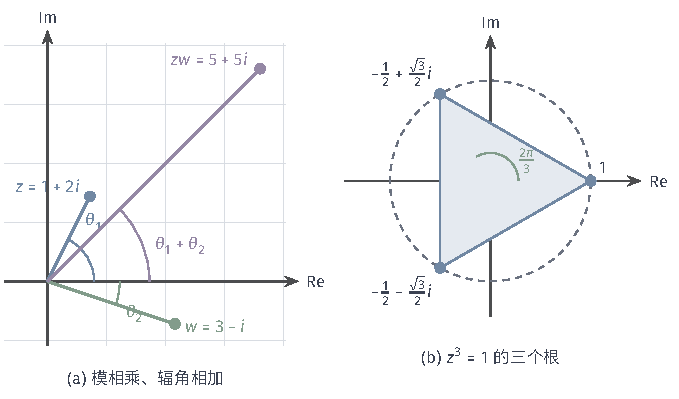
\includegraphics[width=112mm]{figures/01-mathematical-preliminaries-upper/02-real-numbers-and-univariate-functions/tikz/complex-multiplication-roots/figure.pdf}
 \caption{复数乘法与$n$次根的平面表示。(a)蓝、绿两点为$z=1+2i$与$w=3-i$，紫点为乘积$zw=5+5i$。乘积到原点的距离是$\sqrt5\cdot\sqrt{10}$，辐角是两个辐角之和，图中用弧线标出三个辐角。(b)$z^3=1$的三个根$1$与$-\tfrac12\pm\tfrac{\sqrt3}{2}i$都在单位圆上，辐角依次相差$2\pi/3$，构成正三角形的顶点。}
 \label{fig:ru-complex-multiplication}
\end{figure}

反复使用乘法公式并对$n$归纳，得到正整数次幂
\[
 z^n=r^n(\cos n\theta+i\sin n\theta).
\]
由$z\cdot r^{-1}(\cos(-\theta)+i\sin(-\theta))=1$，$z^{-1}$的模为$r^{-1}$、辐角为$-\theta$，所以公式对负整数次幂也成立。

反过来求$n$次根，就是找$w$使$w^n=z$。设$z=r(\cos\theta+i\sin\theta)$，$r>0$，$w=\rho(\cos\varphi+i\sin\varphi)$。
由幂公式，$w^n=z$要求$\rho^n=r$，并且$n\varphi$与$\theta$相差$2\pi$的整数倍。于是$\rho=r^{1/n}$，
\[
 \varphi=\frac{\theta+2k\pi}{n},\qquad k=0,1,\ldots,n-1.
\]
这$n$个辐角互不相差$2\pi$的整数倍，给出$n$个不同的根；$k$取其他整数时只是重复这些根。
它们到原点的距离相同，辐角依次相差$2\pi/n$，恰好是一个正$n$边形的顶点。
例如$z=1$时$r=1$、$\theta=0$，三次根为$1$与$\cos(2\pi/3)\pm i\sin(2\pi/3)=-\tfrac12\pm\tfrac{\sqrt3}2i$，如图~\ref{fig:ru-complex-multiplication}(b)。
三角形式中的$\cos\theta+i\sin\theta$还可以写成指数形式，那需要先用级数定义复指数，留到第~\ref{sec:ru-trig-expansion-complex-exponential}节。

\section{函数}
\label{sec:ru-functions}

第~\ref{sec:prelim-functions-value-ranges}节的映射可以在任意集合之间建立对应。本节集中考察输入和输出都是实数的映射，
并把三件容易混在一起的事分开：函数本身是什么，函数怎样被写出来，以及怎样由已有函数得到新函数。

\subsection{函数的定义}
\label{sec:ru-function-definition}

设$X\subseteq\mathbb R$。映射$f:X\to\mathbb R$称为实变量的实值\term{函数}（function），$X$是它的\term{定义域}（domain），$\mathbb R$是目标集。
实际取到的值组成像集$f(X)=\{f(x):x\in X\}$，有序对组成的集合$\{(x,f(x)):x\in X\}$称为函数的\term{图像}（graph）。
两个函数相等，要求定义域相同，并且在每个输入处取值相同。
所以同一个表达式配上不同的定义域，就是不同的函数：$x\mapsto x^2$在$\mathbb R$上不是单射，因为$(-1)^2=1^2$；
限制到$[0,+\infty)$上却是单射，后面正是用这种限制构造平方根。

函数可以用公式写出，如$f(x)=x^2$；也可以分段规定，如
\[
 |x|=\begin{cases}x,&x\geq0,\\-x,&x<0.\end{cases}
\]
集合$A\subseteq\mathbb R$的\term{指示函数}（indicator function）$\mathbb I_A$在$A$上取$1$、在其余位置取$0$；
$\mathbb I_{[0,+\infty)}$也写作$\mathbb I\{x\geq0\}$，称为\term{阶跃函数}（step function），它在原点从$0$跳到$1$。
函数还可以由数据表给出，只列出有限个输入处的值。
有限个值不能确定整个函数：$f(x)=x$与$g(x)=x+\sin(\pi x)$在每个整数处取值相同，因为$\sin(k\pi)=0$，
而在$x=1/2$处一个取$1/2$、一个取$3/2$。所以“与数据表一致”只限制了表中的输入，表外的值还需要别的信息。

公式中常同时出现两类字母。在$f(x)=ax+b$中，$x$是输入，取遍定义域；$a,b$在一次讨论中固定，换一组值就换了一个函数。
后一类字母称为参数，把参数取遍某个集合，就得到一族函数。下面用这个例子区分参数、整个函数、输入和函数值。

\paragraph{函数族与参数化}
\label{sec:prelim-function-families}
设想由输入预测输出：事先并不知道哪条规则最合适，通常先划定一批候选规则，再从中挑选。
这批候选规则本身是一个集合，它的元素是整个函数。具有同一定义域和目标集的一组函数组成\term{函数族}（family of functions）。
例如，形如$f(x)=ax+b$的函数称为一元\term{仿射函数}（affine function），所有这样的函数组成
\[
 \mathcal F=\{f_{a,b}:\mathbb R\to\mathbb R:\ f_{a,b}(x)=ax+b,\ (a,b)\in\mathbb R^2\}.
\]
族中的每个元素是一整个函数。取$(a,b)=(2,1)$得到函数$f_{2,1}(x)=2x+1$；再取输入$x=3$，才得到一个函数值$f_{2,1}(3)=7$。

用参数为函数族中的函数编号，称为\term{参数化}（parameterization），一般写成$\theta\mapsto f_\theta$，其中$\theta$属于参数集合$\Theta$。
这个映射的输入是参数，输出是函数；函数$f_\theta$自身的输入仍是$x$。
参数化把“在函数中挑选”改写为“在参数集合中挑选”，参数集合通常是$\mathbb R^2$这样熟悉的集合，便于后续用数值方法比较和调整。

不同参数可能表示同一个函数，所以参数与函数未必一一对应。能否由函数反过来确定参数，取决于下面的条件。
\begin{definition}[函数参数化的可识别性]
\label{def:prelim-identifiable-parameterization}
给定参数集合$\Theta$与函数族$\{f_\theta:X\to Y:\theta\in\Theta\}$。若$f_\theta=f_{\theta'}$蕴含$\theta=\theta'$，即$\theta\mapsto f_\theta$为单射，
则称这一参数化\term{可识别}（identifiable）；否则称为不可识别。
\end{definition}
这里比较的是整个定义域上的函数，而不是几个位置的函数值。仿射函数族中$b=f_{a,b}(0)$、$a=f_{a,b}(1)-f_{a,b}(0)$，
所以完整函数唯一确定$(a,b)$，这一参数化可识别。若只观察$x=0$处的函数值，则只能确定$b$，不能确定$a$。
可见“完整函数能否确定参数”与“有限个观测能否确定参数”是两个不同的问题。

\Needspace{11\baselineskip}
\begin{example}[参数不同而函数相同]
\label{ex:prelim-nonidentifiable-parameterization}
考虑参数化函数
\[
 f_{a,b}:\mathbb R\to\mathbb R,\qquad f_{a,b}(x)=abx,\qquad(a,b)\in\mathbb R^2.
\]
参数$(1,2)$与$(2,1)$不同，却对每个$x$给出相同的函数值。更一般地，只要$c\neq0$，$(ca,b/c)$与$(a,b)$就表示同一个函数。
从完整的输入输出关系可以确定乘积$ab=f_{a,b}(1)$，却不能分别确定$a$和$b$。这是参数化本身不可识别，而不是计算精度不足。
\end{example}

图~\ref{fig:vol1-add-parameter-function-value}把“由参数得到函数”和“由函数得到函数值”这两层操作分开：三组不同参数先汇入同一条完整规则，然后才在指定的$x$处求值。
\begin{figure}[!htb]
 \centering
 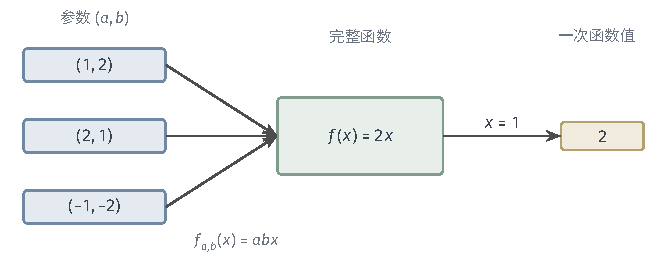
\includegraphics[width=112mm]{figures/01-mathematical-preliminaries-upper/00-shared/tikz/mathematical-language-combinatorics-analysis-optimization-comprehension-additions/parameter-function-value.pdf}
 \caption{参数化$f_{a,b}(x)=abx$中的三层对象。参数$(1,2),(2,1),(-1,-2)$的乘积均为$2$，所以它们表示同一个函数$f(x)=2x$；再指定$x=1$，才得到一次求值结果$2$。多组参数汇入同一完整函数，正是不可识别性。}
 \label{fig:vol1-add-parameter-function-value}
\end{figure}

不可识别的参数可以用第~\ref{sec:prelim-equivalence-relations}节的等价关系整理。规定$\theta\sim\theta'$当且仅当$f_\theta=f_{\theta'}$，
函数相等本身是自反、对称、传递的，所以$\sim$是参数集合上的等价关系。
每个等价类收集同一个函数的全部参数表示；在$f_{a,b}(x)=abx$中，$(a,b)$所在的等价类是满足$a'b'=ab$的全部$(a',b')$。
把每个等价类对应到它所表示的函数，得到商集$\Theta/{\sim}$到函数族的双射；参数化可识别，恰好意味着每个等价类只含一个参数。
统计模型中由有限样本推断参数时的可识别性，留到推断部分讨论。

\subsection{函数的运算}
\label{sec:ru-function-arithmetic}
\label{sec:real-function-arithmetic}

若$f,g:X\to\mathbb R$有相同的定义域，可以在每个输入处对两个函数值做实数运算：
\[
 (f\pm g)(x)=f(x)\pm g(x),\qquad (fg)(x)=f(x)g(x),\qquad (cf)(x)=cf(x),
\]
其中$c$为实常数，这些新函数的定义域仍是$X$。商只在分母不为零的输入上定义：$(f/g)(x)=f(x)/g(x)$的定义域为$\{x\in X:g(x)\neq0\}$。
例如在$\mathbb R$上取$f(x)=x$、$g(x)=x-1$，则$(f+g)(x)=2x-1$定义在整条实轴上，$(f/g)(x)=x/(x-1)$的定义域却不含$1$。
两个函数的定义域不同时，先取公共部分再运算。这些运算都作用在输出值上，与下面的复合不同。

复合把一个函数的输出送入另一个函数作为输入。设$f:X\to\mathbb R$，$g:Y\to\mathbb R$，复合$g\circ f$在$x$处的值是$g(f(x))$，
它只对满足$f(x)\in Y$的$x$有意义。例如$f(x)=1-x^2$、$g(y)=\sqrt y$（$y\geq0$），则$(g\circ f)(x)=\sqrt{1-x^2}$的定义域是$[-1,1]$，
因为只有这些$x$使$1-x^2\geq0$。复合一般不能交换次序：$(f\circ g)(y)=1-y$与$(g\circ f)(x)$是完全不同的函数。

反函数要求先有一一对应。平方函数在$\mathbb R$上不是单射，没有反函数；把定义域限制为$[0,+\infty)$后，它是$[0,+\infty)$到$[0,+\infty)$的双射，
其逆映射就是平方根$y\mapsto\sqrt y$。按第~\ref{sec:prelim-map-operations}节，反函数满足$f^{-1}(f(x))=x$与$f(f^{-1}(y))=y$。
把图像上的每个点$(x,y)$换成$(y,x)$，就得到反函数的图像，即原图像关于直线$y=x$的反射：输入与输出互换了位置。

三个记号需要分清。$f^{-1}$在反函数存在时表示反函数，$1/f$表示逐点取倒数，$f^{-1}(B)=\{x:f(x)\in B\}$表示集合的原像，后者对任何函数都有定义。
以限制在$[0,+\infty)$上的平方函数为例，$f^{-1}(4)=2$，$(1/f)(4)=1/16$；而对定义在$\mathbb R$上的平方函数，原像$f^{-1}(\{4\})=\{-2,2\}$是一个集合，它没有反函数。

\section{函数的性质}
\label{sec:prelim-optimal-values-errors}
\label{sec:ru-function-properties}

从候选函数中挑选时，常把每个候选的优劣写成一个实数，再寻找使它最小的候选。这要求我们能够描述一个函数的取值范围、增减方向和对称性，
并分清“最小的值是多少”和“在哪里取到”。本节把实数集合的确界用到函数的像集上，再用输入之间的关系定义单调、奇偶和周期。

设$X$非空，$f:X\to\mathbb R$。函数的有界性就是像集$f(X)$的有界性：若$f(X)$有上界，称$f$上有界，下界与有界同理。
像集的确界简记为
\[
 \sup_{x\in X}f(x)=\sup f(X),\qquad \inf_{x\in X}f(x)=\inf f(X).
\]
若$f(X)$无上界，约定$\sup_Xf=+\infty$；若无下界，约定$\inf_Xf=-\infty$。这两个符号只表示没有有限的界，不是函数实际取到的数。
若存在$x^\star\in X$使$f(x^\star)=\inf_Xf$，就称$f(x^\star)$为$f$的最小值；最大值类似。
例如$f(x)=x$在$(0,1)$上有下确界$0$，却没有最小值：任一允许的输入$x$都有更小的允许输入$x/2$。

若对$X$中任意$x<y$都有$f(x)\leq f(y)$，称$f$单调不减；若总有$f(x)<f(y)$，称$f$严格递增。
单调不增与严格递减类似地定义，它们统称\term{单调函数}（monotone function）。单调性比较的是两个输入及其输出的大小关系，与函数能否用公式写出无关。

奇偶性与周期性描述输入变换下函数值的不变性。若定义域关于原点对称（$x\in X$蕴含$-x\in X$），并且$f(-x)=f(x)$，称$f$为偶函数，图像关于纵轴对称；
若$f(-x)=-f(x)$，称$f$为奇函数，图像关于原点对称。定义域不对称时谈不上奇偶：$x^2$在$[0,1]$上不是偶函数，因为$-1/2$不在定义域中。
若存在$T>0$，使$x\in X$蕴含$x+T\in X$且$f(x+T)=f(x)$，称$f$以$T$为周期；平移输入$x\mapsto x-c$则把图像整体右移$c$。
这些性质都依赖定义域，讨论时须把定义域与表达式一起写明。

严格单调还带来可逆性。若$f$在$X$上严格递增，则$x\neq y$时$f(x)\neq f(y)$，$f$是$X$到像集$f(X)$的双射，因而有反函数$f^{-1}:f(X)\to X$。
反函数仍严格递增：若$u<v$属于$f(X)$而$f^{-1}(u)\geq f^{-1}(v)$，两边作用$f$便得$u\geq v$，矛盾。
这里只得到了反函数的存在与单调性；反函数是否连续，要等下一章有了连续性的概念才能讨论。

\paragraph{最小值与最小点}
寻找最小值时，答案包含两部分：最小的函数值是多少，以及哪些输入取到它。若$x^\star\in X$满足
\[
 f(x^\star)\leq f(x)\qquad\text{对所有}\ x\in X,
\]
则称$x^\star$为\term{全局最小点}（global minimizer），$f(x^\star)$为最小值，记作$\min_{x\in X}f(x)$。全部最小点组成的集合记作
\[
 \argmin_{x\in X}f(x)=\{x\in X:\ f(x)\leq f(z)\ \text{对所有}\ z\in X\}.
\]
$\min$给出一个数，$\argmin$给出输入的集合；若不存在最小点，后一个集合为空。
把不等号反向，就得到全局最大点、最大值$\max_{x\in X}f(x)$与集合$\argmax_{x\in X}f(x)$。

最小值存在时必等于下确界：$f(x^\star)$不超过每个函数值，所以是像集的下界；任何下界$m$都满足$m\leq f(x^\star)$，因为$f(x^\star)$本身就是一个函数值。
反过来，下确界存在却未必被取得，前面$(0,1)$上的$f(x)=x$就是例子。
图~\ref{fig:prelim-minimum-infimum}比较同一表达式在$(0,1)$与$[0,1]$上定义的两个函数：区别在于边界点是否属于定义域，而不在于曲线趋向什么高度。

\begin{figure}[htbp]
 \centering
 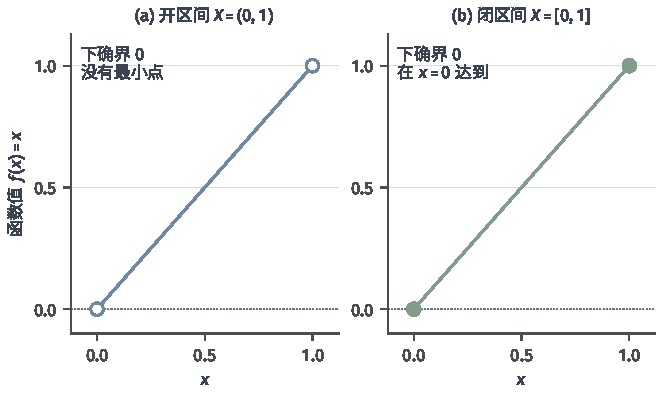
\includegraphics[width=112.0mm]{figures/01-mathematical-preliminaries-upper/01-mathematical-language-combinatorics-analysis-optimization/matplotlib/prelim-minimum-infimum/figure.pdf}
 \caption{同一求值表达式$f(x)=x$在两个定义域上的边界对照。左图定义域为$(0,1)$，空心端点不属于图像，函数值可任意接近$0$，却不能取到；右图定义域为$[0,1]$，实心端点$(0,0)$达到下确界。两图的下确界相同，最小点是否存在取决于可行端点是否保留。图为解析教学示例。}
 \label{fig:prelim-minimum-infimum}
\end{figure}

最小值唯一，最小点却可以有多个。
\begin{example}[同一个最优值可以对应多个输入]
\label{ex:prelim-optimal-value-versus-points}
令$X=[-2,2]$，$f(x)=(x^2-1)^2$。平方非负，且$x=\pm1$都使它为零，所以
\[
 \min_{x\in X}f(x)=\inf_{x\in X}f(x)=0,\qquad \argmin_{x\in X}f(x)=\{-1,1\}.
\]
又因为$0\leq x^2\leq4$，有$|x^2-1|\leq3$，于是$f(x)\leq9$，等号恰在$x=\pm2$处成立，最大值为$9$，最大点集合为$\{-2,2\}$。
\end{example}
例子说明，两个最小点给出的是同一个最小值；最优值相同，并不意味着最优点唯一。怎样求出最小点，是最优化部分的问题，这里只确定它们是什么。

\section{基本函数}
\label{sec:ru-elementary-functions}

后面的例子反复用到几类具体函数：多项式与有理函数、幂函数、指数与对数、三角函数及其反函数。
它们在中学已经出现过，本节只复习怎样辨认它们、它们允许哪些输入，以及常用的恒等式；严格的构造与分析性质留给后两章。

形如$p(x)=c_0+c_1x+\cdots+c_nx^n$的函数称为\term{多项式}（polynomial），它对每个实数$x$都有定义；
两个多项式之商$p(x)/q(x)$称为有理函数，定义域要去掉$q$的零点。幂函数$x^\alpha$的允许输入取决于指数：
正整数次幂对所有$x$有定义；负整数次幂如$x^{-1}=1/x$要求$x\neq0$；$x^{1/2}=\sqrt x$只对$x\geq0$取实数值；
指数$\alpha$不是有理数时，$x^\alpha$只对$x>0$定义，第~\ref{sec:ru-elementary-derivatives}节将用指数和对数给出它的定义。
所以同一个记号$x^\alpha$，定义域会随$\alpha$改变。

设$a>0$且$a\neq1$。指数函数$a^x$对所有实数$x$有定义，取值恒为正，满足$a^{x+y}=a^xa^y$、$(a^x)^y=a^{xy}$；
$a>1$时它严格递增，$0<a<1$时严格递减。由上一节，严格单调的函数有反函数，指数函数的反函数就是以$a$为底的对数$\log_ax$，定义域为$(0,+\infty)$。
两者互为反函数，意味着$a^{\log_ax}=x$（$x>0$）与$\log_a(a^x)=x$（$x\in\mathbb R$），由此得到$\log_a(xy)=\log_ax+\log_ay$。
底数取$e\approx2.71828$时，$e^x$称为自然指数函数，其反函数记作$\log x$（也记$\ln x$），称为自然对数；本书不加底数的$\log$都指自然对数。
底数为何要求$a>0$：负数的分数次幂可能不是实数，例如$(-1)^{1/2}$；$a=1$时$1^x\equiv1$不是单射，没有反函数。

三角函数通过单位圆定义。从点$(1,0)$出发，沿单位圆逆时针走过弧长$\theta$，到达的点记作$(\cos\theta,\sin\theta)$；
$\theta<0$时顺时针走。用弧长度量角称为弧度制，一周的弧长为$2\pi$。由这一定义，$\cos^2\theta+\sin^2\theta=1$，
正弦和余弦以$2\pi$为周期，正弦是奇函数、余弦是偶函数。正切$\tan\theta=\sin\theta/\cos\theta$要求$\cos\theta\neq0$，即$\theta\neq\pi/2+k\pi$，它以$\pi$为周期。
加法公式
\[
 \sin(\alpha+\beta)=\sin\alpha\cos\beta+\cos\alpha\sin\beta,\qquad
 \cos(\alpha+\beta)=\cos\alpha\cos\beta-\sin\alpha\sin\beta
\]
在复数乘法中已经用过，后面求三角函数的导数时还要用到。

三角函数是周期函数，在整个定义域上不是单射。要得到反函数，须先选一个函数严格单调、并取遍全部函数值的区间。
正弦在$[-\pi/2,\pi/2]$上从$-1$严格增到$1$，它在这一区间上的反函数记作$\arcsin:[-1,1]\to[-\pi/2,\pi/2]$；
余弦在$[0,\pi]$上从$1$严格减到$-1$，相应的反函数为$\arccos:[-1,1]\to[0,\pi]$；正切在$(-\pi/2,\pi/2)$上严格递增，反函数为$\arctan:\mathbb R\to(-\pi/2,\pi/2)$。
例如$\sin(5\pi/6)=1/2$，但$\arcsin(1/2)=\pi/6$，因为$5\pi/6$不在选定的区间内。表~\ref{tab:ru-elementary-functions}汇总这些函数的定义域、值域与周期。

\begin{table}[htbp]
 \centering\small
 \begin{tabular}{@{}llll@{}}
 \toprule
 函数 & 定义域 & 值域 & 周期\\
 \midrule
 $x^n$（$n$为正奇数/偶数） & $\mathbb R$ & $\mathbb R$\,/\,$[0,+\infty)$ & \\
 $x^{-n}$（$n$为正奇数/偶数） & $x\neq0$ & $x\neq0$\,/\,$(0,+\infty)$ & \\
 $\sqrt x$ & $[0,+\infty)$ & $[0,+\infty)$ & \\
 $a^x$（$a>0$，$a\neq1$） & $\mathbb R$ & $(0,+\infty)$ & \\
 $\log_ax$（$a>0$，$a\neq1$） & $(0,+\infty)$ & $\mathbb R$ & \\
 $\sin x$，$\cos x$ & $\mathbb R$ & $[-1,1]$ & $2\pi$\\
 $\tan x$ & $x\neq\pi/2+k\pi$ & $\mathbb R$ & $\pi$\\
 $\arcsin x$ & $[-1,1]$ & $[-\pi/2,\pi/2]$ & \\
 $\arccos x$ & $[-1,1]$ & $[0,\pi]$ & \\
 $\arctan x$ & $\mathbb R$ & $(-\pi/2,\pi/2)$ & \\
 \bottomrule
 \end{tabular}
 \caption{基本函数的定义域、值域与周期。斜线前后分别对应奇数与偶数次幂；$\sqrt x$是平方函数在$[0,+\infty)$上的反函数，$a^x$与$\log_ax$互为反函数。三角函数采用弧度制，$\log$不写底数时指自然对数。}
 \label{tab:ru-elementary-functions}
\end{table}

需要说明这些描述依赖什么。上面把指数函数当作已知对象使用，但“$a^x$对无理数$x$是什么数”“$e$是什么数”都需要极限才能回答；
单位圆上的弧长、$\sin h$与$h$在$h$很小时的比较，也需要极限。
下一章将先用级数构造自然指数函数，由代数和估计得到它的正性、单调性与加法公式，
在介值定理之后严格构造自然对数，并证明三角函数的基本极限；第~\ref{sec:ru-euler-formula}节再由级数得到Euler公式。
在那之前，本节的内容只作为辨认和计算的背景，不用来论证无限求和、连续性或指数与三角函数的关系。

\section{数列与有限求和}
\label{sec:ru-sequences-finite-sums}

数列是以自然数为输入的函数。把它单独列出，是因为下一章的极限首先在数列上定义，而无限求和又要从有限和出发。
本节说明数列与集合、函数族的区别，再推导几类不需要极限的有限和公式。

一个实数\term{数列}（sequence）就是映射$a:\{1,2,\ldots\}\to\mathbb R$，把$n$处的值写作$a_n$，整个数列记作$(a_n)_{n\geq1}$或$(a_n)$；有时下标从$0$开始。
数列记录了每一项的位置，因而与它的取值集合不同：数列$((-1)^n)$在$-1$与$1$之间无限次交替，取值集合$\{-1,1\}$却只有两个元素，次序和重复都看不出来。
数列也不同于函数族：数列的每一项是一个数，函数族的每个元素是一整个函数。下一章研究函数列时，每个编号对应的才是一个函数。

第~\ref{sec:prelim-finite-sums-products}节已经约定了有限和$\sum_{k=1}^na_k$与有限积的记号，这里只回顾三条后面常用的规则。
平移哑索引时范围随之改写，如$\sum_{k=1}^{n}a_{k+1}=\sum_{j=2}^{n+1}a_j$；空和为$0$、空积为$1$，使拆分求和时不必单独处理空的部分；
有限个项的二重和可以交换次序，内层范围依赖外层索引时按式~\eqref{eq:prelim-triangular-sum}重写范围。
交换次序的依据是每个索引对恰好被计入一次，这只对有限多项成立；无限多项的和要先用极限定义，第~\ref{sec:ru-series-rearrangement-grouping}节将看到交换次序可能改变结果。

几类有限和可以直接写出公式。先看$\sum_{k=1}^nk$：把它正着写一遍、倒着写一遍再逐项相加，每一对都等于$n+1$，共$n$对，所以
\[
 \sum_{k=1}^nk=\frac{n(n+1)}2.
\]
由此得到首项为$a$、公差为$d$的等差数列前$n$项之和：
\[
 \sum_{k=0}^{n-1}(a+kd)=na+d\sum_{k=0}^{n-1}k=na+\frac{n(n-1)}2d.
\]
公比为$\rho$的几何和由式~\eqref{eq:prelim-finite-geometric-sum}给出：$\rho\neq1$时$\sum_{k=0}^N\rho^k=(1-\rho^{N+1})/(1-\rho)$，$\rho=1$时为$N+1$。
两个公式都要写清首项、项数和公比；求和从$k=1$开始时，几何和要再乘一个$\rho$。

若每一项能写成相邻两项之差$a_k=b_k-b_{k+1}$，式~\eqref{eq:prelim-telescoping-sum}给出$\sum_{k=1}^Na_k=b_1-b_{N+1}$，中间各项两两抵消，称为裂项求和。
例如$\frac1{k(k+1)}=\frac1k-\frac1{k+1}$，所以
\[
 \sum_{k=1}^N\frac1{k(k+1)}=1-\frac1{N+1}.
\]
这些恒等式对每个固定的$N$成立，只用到有限次运算。当$N$无限增大时，$1-1/(N+1)$与$(1-\rho^{N+1})/(1-\rho)$会怎样变化，下一章用极限回答。


\FloatBarrier
\section{本章小结}
\label{sec:real-complex-functions-summary}

实数部分只做了三件事：用区间和绝对值描述位置与距离，用确界原理保证有界集合有最小上界或最大下界，
再由确界原理得到Archimedes性、有理数的稠密性和闭区间套性质。十进制表示正是闭区间套的一个实例。
复数部分则把$i^2=-1$加入运算，四则运算由实部、虚部逐项计算，除法借助共轭化为实数分母；
在平面上，乘法表现为模相乘、辐角相加。下一章判断极限是否存在时，依靠的是实数的完备性，而不是数值图像。

函数部分区分了函数本身与它的表示：同一表达式在不同定义域上给出不同函数，参数确定函数族中的一个成员，有限个函数值却不能确定整个函数。
最小值是一个数，最小点是输入的集合；下确界存在时，最小值未必存在。
数列是以自然数为输入的函数，有限求和的等差、几何与裂项公式都不需要极限。
到这里为止，误差都是有限步内的数值。项数无限增大、输入无限靠近时会发生什么，是下一章的问题。

\chapter{极限与连续}
\label{chap:limits-continuity}
\label{chap:function-limits}
\label{chap:mathematical-analysis}

第~\ref{chap:sets-relations-maps}章的等比递推给出了有限步结果$e^{(t)}=\rho^te_0$，上一章又算出了有限几何和与裂项和。
当$t$或项数无限增大时，这些数是否趋向确定的值？输入无限靠近某一点时，函数值又趋向哪里？
回答这类问题，先要说清“趋近”的含义，再判断在什么条件下趋近确实产生一个确定的结果，以及这种结果能否与加减乘除、复合等运算交换次序。

本章的主线从数列出发。数列极限用误差条件定义，我们分别讨论已知收敛时怎样计算极限、不知道极限值时怎样保证极限存在，后者要用到上一章的确界原理。
级数是部分和组成的数列，数列的结论由此用于无限多项的累计，并引出重排与分组这些有限和中不会出现的问题。
随后把极限推广到实变量函数，用函数极限定义连续性，并在闭区间上证明最值、介值和一致连续这几条整体性质。
最后一步让函数本身随编号变化：函数列与函数项级数何时保持连续性，以及幂级数在哪些输入处收敛。
本章只使用实轴上的距离$|x-y|$，一般距离下的相应理论在第~\ref{chap:metric-spaces}章统一讨论。

\section{数列的极限}
\label{sec:ru-sequence-limits}
\label{sec:analysis-continuous-limits}
\label{sec:analysis-sequences-series-errors}

数列$1,1/2,1/3,\ldots$越来越接近$0$，数列$-1,1,-1,1,\ldots$则在两个值之间来回交替。
直觉上前者“有极限”，后者没有；但“越来越接近”需要精确的含义，否则无法判断$(1+1/n)^n$或$\sum_{k\leq n}1/k$这类数列是否趋向某个数。
本节先用误差条件定义收敛并建立极限的运算，再给出不必事先知道极限值的存在性判别，最后描述趋向无穷和不收敛数列的尾部行为。

\subsection{收敛、发散与极限运算}
\label{sec:ru-convergence-limit-laws}

比较$(1/n)$与$((-1)^n)$，区别在于尾部。$1/n$从某一项起全部落在$0$附近任意窄的范围内；$((-1)^n)$的偶数项都等于$1$，奇数项却始终离$1$有距离$2$。
所以“接近一个数”必须约束后面的\emph{每一项}。只要求“各项离$a$越来越近”也不够：$1+1/n$离$0$越来越近，却始终大于$1$。
合适的要求是：无论事先给定多小的正误差，从某一项起，后面每一项与$a$的距离都小于这个误差。

\begin{definition}[数列的极限]
\label{def:ru-sequence-limit}
设$(a_n)$为实数列，$a\in\mathbb R$。若对每个$\varepsilon>0$，都存在正整数$N$，使
\[
 n\geq N\quad\Longrightarrow\quad|a_n-a|<\varepsilon,
\]
就称$(a_n)$\term{收敛}（converge）到$a$，$a$称为它的极限，记作$\lim_{n\to\infty}a_n=a$或$a_n\to a$。没有实数极限的数列称为\term{发散}（diverge）。
\end{definition}

定义中的量词次序不能交换：先任给误差$\varepsilon$，再选取尾部起点$N$。$N$可以依赖于$\varepsilon$，误差要求越严格，所需的起点通常越靠后。
极限也不要求某一项恰好等于$a$\scite{math-lebl-analysis1}。
例如对$a_n=1/n$，任给$\varepsilon>0$，由Archimedes性取正整数$N>1/\varepsilon$，则$n\geq N$时$|1/n-0|\leq1/N<\varepsilon$，所以$1/n\to0$。
图~\ref{fig:analysis-process-sequence-tail}把“全部尾部项”画成同一条误差带。

\begin{figure}[!htbp]
 \centering
 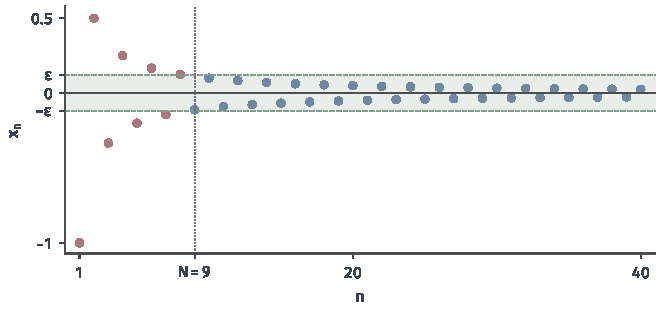
\includegraphics[width=112.0mm]{figures/01-mathematical-preliminaries-upper/00-shared/matplotlib/chapter3-concept-processes/sequence-tail.pdf}
 \caption{数列$x_n=(-1)^n/n$的前40项。绿色带为$|x_n|<0.12$，取$N=9$后，所有$n\geq9$都在带内；蓝点标记这个尾部，红点标记之前的项。尾部条件针对无限多个$n$，其成立依据是$1/n\leq1/9<0.12$，不是只检查图中有限个点。}
 \label{fig:analysis-process-sequence-tail}
\end{figure}

要说明$a_n$不收敛到$a$，须写出定义的否定：存在某个$\varepsilon_0>0$，使得无论$N$取多大，总有$n\geq N$满足$|a_n-a|\geq\varepsilon_0$。
对$((-1)^n)$，取$\varepsilon_0=1$：相邻两项相差$2$，不可能同时落在长度为$2$的开区间$(a-1,a+1)$内，所以它不收敛到任何$a$，是发散数列。

定义需要先给出一个候选极限$a$，那么会不会有两个候选都满足定义？不会。若$a\neq b$都是极限，取$\varepsilon=|a-b|/3$，充分靠后的项同时满足$|a_n-a|<\varepsilon$和$|a_n-b|<\varepsilon$，
三角不等式却给出$|a-b|\leq|a-a_n|+|a_n-b|<2|a-b|/3$，矛盾。所以收敛数列的极限唯一，记号$\lim a_n$表示一个确定的数。

定义只控制尾部，而尾部之前只有有限个项，因此收敛数列必有界。设$a_n\to a$，取$\varepsilon=1$得到$N$，使$n\geq N$时$|a_n|<|a|+1$；
再令$M=\max\{|a_1|,\ldots,|a_{N-1}|,|a|+1\}$，就有$|a_n|\leq M$对所有$n$成立。
反过来不成立，$((-1)^n)$有界却不收敛。这一性质常以逆否形式使用：无界数列一定发散。

已知几个数列收敛时，由它们组合出的数列的极限可以直接算出。思路都是把新数列的误差拆成已知误差的组合。
\begin{theorem}[数列极限的四则运算]
\label{thm:ru-sequence-limit-laws}
设$a_n\to a$，$b_n\to b$，其中$a,b\in\mathbb R$，$c$为实常数，则
\[
 a_n\pm b_n\to a\pm b,\qquad ca_n\to ca,\qquad a_nb_n\to ab.
\]
若还有$b\neq0$，则充分靠后的$b_n\neq0$，并且$a_n/b_n\to a/b$。
\end{theorem}
\begin{proof}
和与差由$|(a_n\pm b_n)-(a\pm b)|\leq|a_n-a|+|b_n-b|$得到：让两个误差各小于$\varepsilon/2$即可。数乘的误差是$|c|\,|a_n-a|$，同样可以任意小。

乘积的误差含有一个变化的因子，需要用到收敛数列的有界性。取$M\geq1$使所有$|a_n|\leq M$，则
\[
 |a_nb_n-ab|=|a_n(b_n-b)+b(a_n-a)|\leq M|b_n-b|+|b|\,|a_n-a|,
\]
让$|b_n-b|<\varepsilon/(2M)$与$|a_n-a|<\varepsilon/[2(|b|+1)]$同时成立，右侧便小于$\varepsilon$。

对商，先取误差$|b|/2$，得知充分靠后的$|b_n|\geq|b|/2>0$。于是
\[
 \Bigl|\frac1{b_n}-\frac1b\Bigr|=\frac{|b_n-b|}{|b_n|\,|b|}\leq\frac{2|b_n-b|}{|b|^2}\to0,
\]
前面有限个项不影响极限，再对$a_n\cdot(1/b_n)$用乘积规则。
\end{proof}
例如把分子分母同除以$n$，得$n/(n+1)=1/(1+1/n)\to1$。分母极限为零时不能套用商的规则：$0/0$与$\infty-\infty$都不是可以直接计算的数值，须先变形。

有时一个数列不断振荡，直接控制它的误差并不方便，但能找到两个趋向同一值的上下界。
\begin{theorem}[夹逼定理]
\label{thm:analysis-sequence-squeeze}
设实数列满足：存在$N_0$使$n\geq N_0$时$a_n\leq c_n\leq b_n$，并且$a_n\to\ell$、$b_n\to\ell$，其中$\ell\in\mathbb R$，则$c_n\to\ell$。
\end{theorem}
\begin{proof}
任给$\varepsilon>0$，取$N\geq N_0$使$n\geq N$时$|a_n-\ell|<\varepsilon$且$|b_n-\ell|<\varepsilon$。于是$\ell-\varepsilon<a_n\leq c_n\leq b_n<\ell+\varepsilon$，即$|c_n-\ell|<\varepsilon$。
\end{proof}
例如$-1/n\leq(\sin n)/n\leq1/n$，所以$(\sin n)/n\to0$。

等比数列$(r^n)$是反复出现的例子，夹逼定理可以判定它的全部情形。$r=0$时显然趋于零。若$0<|r|<1$，写$1/|r|=1+h$，$h>0$。
对$n$归纳可证$(1+h)^n\geq1+nh$：$n=1$时取等号；若对$n$成立，则$(1+h)^{n+1}\geq(1+nh)(1+h)\geq1+(n+1)h$。
因此$0<|r|^n\leq1/(1+nh)<1/(nh)\to0$，再对$-|r|^n\leq r^n\leq|r|^n$用夹逼定理，得到$r^n\to0$。
$r=1$时各项恒为$1$，收敛；$r=-1$时在$\pm1$间交替，发散；$|r|>1$时同一不等式给出$|r|^n\geq1+nh$（其中$|r|=1+h$），数列无界，因而发散。
回到等比递推~\eqref{eq:prelim-geometric-recurrence}：设$e_0\neq0$，$e^{(t)}=\rho^te_0$恰在$|\rho|<1$时趋于零，在$\rho=1$时保持不变，其余情形发散。

\subsection{极限存在的判别}
\label{sec:ru-limit-existence}

定义收敛时需要先给出候选极限，但很多数列的极限值事先并不知道。下面依次利用变化方向、取值范围和尾部各项的相互接近来判断极限是否存在。

若对所有$n$都有$a_n\leq a_{n+1}$，称数列单调不减；若总有$a_n\geq a_{n+1}$，称数列单调不增，两者统称单调数列。
单调不减且有上界的数列，全部项的集合有上确界；单调性又保证后面的项一直靠近它。
\begin{theorem}[单调有界收敛定理]
\label{thm:analysis-monotone-bounded-sequence}
单调不减且有上界的实数列收敛，极限为$\sup\{a_n:n\geq1\}$；单调不增且有下界的实数列收敛，极限为$\inf\{a_n:n\geq1\}$。
\end{theorem}
\begin{proof}
设$a=\sup\{a_n:n\geq1\}$，它由确界原理保证存在。给定$\varepsilon>0$，$a-\varepsilon$不是上界，所以存在$N$使$a_N>a-\varepsilon$。
单调性使$n\geq N$时$a-\varepsilon<a_N\leq a_n\leq a$，这正是$a_n\to a$。单调不增的情形对$-a_n$应用同一论证。
\end{proof}
两个条件都不能省去：$(n)$单调却无上界，$((-1)^n)$有界却不单调。结合收敛数列的有界性，单调数列收敛当且仅当它有界。

有界数列未必收敛，但其中可能有一部分项具有共同的趋向。若$n_1<n_2<\cdots$为严格递增的正整数列，则$(a_{n_k})_{k\geq1}$称为$(a_n)$的\term{子列}（subsequence），由归纳可知$n_k\geq k$。
收敛数列的每个子列都收敛到同一极限：若$n\geq N$时$|a_n-a|<\varepsilon$，则$k\geq N$时$n_k\geq k\geq N$，同一误差界仍然适用。
\begin{theorem}[Bolzano--Weierstrass定理]
\label{thm:analysis-bounded-subsequence}
有界实数列必有收敛子列。
\end{theorem}
\begin{proof}
设$|a_n|\leq M$。从包含全部项的闭区间$I_0=[-M,M]$出发，将它平分；两半中至少有一半含有无穷多个下标对应的项，选出这一半。
重复平分与选择，得到嵌套闭区间$I_0\supseteq I_1\supseteq\cdots$，其中每个$I_k$都含有无穷多项，长度为$2M\cdot2^{-k}$。
由于每个$I_k$都含有无穷多项，可以依次选取下标$n_1<n_2<\cdots$使$a_{n_k}\in I_k$。
由$2^k\geq k+1$，区间长度可以任意小，闭区间套性质给出唯一公共点$c$。$a_{n_k}$与$c$都在$I_k$中，所以$|a_{n_k}-c|\leq2M\cdot2^{-k}\to0$。
\end{proof}
“有界”只能保证子列收敛，不能保证整列收敛：$((-1)^n)$的偶数项子列收敛到$1$，奇数项子列收敛到$-1$，整列却发散。

单调条件并不适用于所有收敛数列。不知道候选极限时，还可以检查尾部各项是否彼此接近。满足
\[
 \forall\varepsilon>0,\quad\exists N,\quad\forall m,n\geq N,\quad|a_m-a_n|<\varepsilon
\]
的数列称为\term{柯西数列}（Cauchy sequence）。这个条件只涉及数列自身的项，不需要知道极限是多少。
\begin{theorem}[柯西收敛准则]
\label{thm:analysis-cauchy-convergence}
实数列收敛，当且仅当它是柯西数列。
\end{theorem}
\begin{proof}
收敛数列是柯西数列：若$n\geq N$时$|a_n-a|<\varepsilon/2$，则对$m,n\geq N$有$|a_m-a_n|\leq|a_m-a|+|a-a_n|<\varepsilon$。

反过来，先说明柯西数列有界：取误差$1$得到$N$，所有$n\geq N$都满足$|a_n-a_N|<1$，前面有限项另取最大绝对值即可。
由Bolzano--Weierstrass定理，可取子列$a_{n_k}\to a$。给定$\varepsilon>0$，选$N$使$m,n\geq N$时$|a_m-a_n|<\varepsilon/2$，再选$k$使$n_k\geq N$且$|a_{n_k}-a|<\varepsilon/2$。
于是每个$n\geq N$都有$|a_n-a|\leq|a_n-a_{n_k}|+|a_{n_k}-a|<\varepsilon$。
\end{proof}
充分性经过收敛子列，因而仍然依赖确界原理。在有理数中，$\sqrt2$的十进制截断$1,1.4,1.41,\ldots$是柯西数列，却没有有理数极限。

验证柯西条件时，可把两个较晚的项之间的距离估计为逐步变化的总和：对$m>n$，
\begin{equation}
 |a_m-a_n|\leq\sum_{k=n}^{m-1}|a_{k+1}-a_k|.
 \label{eq:analysis-cauchy-tail-bound}
\end{equation}
只看相邻两项不够，因为中间的步数也在增加。设$a_1=0$、$a_{k+1}-a_k=1/k$，每一步都趋于零；但$a_{2n}-a_n=\sum_{k=n}^{2n-1}1/k$共有$n$项，每项都大于$1/(2n)$，
所以$a_{2n}-a_n>1/2$。它不是柯西数列，因而发散。这里的$a_{n+1}$正是第~\ref{sec:analysis-series}节调和级数的前$n$项和。

\subsection{无穷极限、上极限与下极限}
\label{sec:ru-infinite-limits-limsup}

数列$(n)$发散，但它的发散方式很确定：越过任何有限界以后不再回头。为记录这种趋向，规定$a_n\to+\infty$表示对每个实数$M$，都存在$N$使$n\geq N$时$a_n>M$；
$a_n\to-\infty$则要求最终都有$a_n<M$。趋向$\pm\infty$的数列仍是发散数列，$\pm\infty$不是实数极限。
把这两个符号加入实数，得到扩展实数$\overline{\mathbb R}=\mathbb R\cup\{-\infty,+\infty\}$。其中的运算只在不引起歧义时定义，例如$a+(+\infty)=+\infty$（$a$为实数）；
$\infty-\infty$、$0\cdot\infty$与$\infty/\infty$都没有定义，因为不同的数列组合会给出不同结果，如$(n+1)-n\to1$而$2n-n\to+\infty$。

不收敛的数列仍然可以考察尾部的上下边界。逐渐舍去前项时，尾部下确界只会上升，尾部上确界只会下降，因此可以用单调数列的极限记录它们。
\begin{definition}[上极限与下极限]
\label{def:analysis-liminf-limsup}
对实数列$(a_n)$，定义
\[
 \liminf_{n\to\infty}a_n=\lim_{n\to\infty}\inf_{k\geq n}a_k,\qquad
 \limsup_{n\to\infty}a_n=\lim_{n\to\infty}\sup_{k\geq n}a_k,
\]
分别称为\term{下极限}（limit inferior）与\term{上极限}（limit superior）。尾部无上界时$\sup_{k\geq n}a_k=+\infty$，无下界时尾部下确界为$-\infty$。
\end{definition}
右侧尾部下确界随$n$单调不减，尾部上确界随$n$单调不增，所以两个极限都在扩展实数中存在：单调有界时由单调有界收敛定理得到有限极限，无界时趋于相应的无穷。
每个尾部的下确界不超过同一尾部的上确界，所以总有$\liminf a_n\leq\limsup a_n$。

上、下极限恰好刻画了通常的收敛。若二者都等于有限数$a$，给定$\varepsilon>0$，充分靠后的尾部下确界大于$a-\varepsilon$、尾部上确界小于$a+\varepsilon$，
夹在中间的每个尾部项都满足$|a_n-a|<\varepsilon$，即$a_n\to a$。反之若$a_n\to a$，则$n\geq N$时尾部全落在$(a-\varepsilon,a+\varepsilon)$内，尾部的上下确界都在$[a-\varepsilon,a+\varepsilon]$中。
同理，两者都等于$+\infty$恰好对应$a_n\to+\infty$，都等于$-\infty$对应$a_n\to-\infty$。

两者不相等时，它们记录了数列尾部来回摆动的范围。$((-1)^n)$的下极限为$-1$、上极限为$1$；$((-1)^nn)$的下极限为$-\infty$、上极限为$+\infty$；
$(n(1+(-1)^n))$的奇数项为$0$、偶数项为$2n$，下极限为$0$、上极限为$+\infty$。
对有界数列，上极限还是某个子列的极限：记$L=\limsup a_n$，对每个$j$先取足够晚的起点使其后的尾部上确界小于$L+1/j$，
这一尾部中又有某项大于$L-1/j$；在超过前次所选下标的位置选出这样的项，便得到趋于$L$的子列。下极限同理。

\section{级数的极限}
\label{sec:ru-series}
\label{sec:analysis-series}

有限和可以逐项相加，无限多项却无法“加完”。上一节的数列极限提供了处理办法：把前$N$项的和看成一个数列，再问$N$无限增大时它是否趋向确定的数。
本节先用部分和定义级数及其和，计算几类可作基准的级数；随后建立收敛判别，区分不依赖抵消的绝对收敛与依赖抵消的条件收敛；最后说明改变求和次序或合并相邻项会怎样影响结果。

\subsection{部分和、余项与基本级数}
\label{sec:ru-partial-sums}
\label{sec:analysis-series-definition}

给定数列$(a_n)_{n\geq1}$，称$s_N=\sum_{n=1}^Na_n$为第$N$个\term{部分和}（partial sum）。符号\term{无穷级数}（infinite series）$\sum_{n=1}^\infty a_n$描述这一求和过程；
若部分和数列$(s_N)$有有限极限$s$，称级数收敛，并记$\sum_{n=1}^\infty a_n=s$，称$s$为级数的和；否则称级数发散。
三个对象要分清：单项$a_n$、部分和$s_N$与级数的和$s$。例如$a_n=2^{-n}\to0$，而$s_N=1-2^{-N}\to1$。

由$a_N=s_N-s_{N-1}$及差的极限法则，级数收敛必须有$a_N\to0$。反向不成立：上一节末尾的例子说明调和级数$\sum1/n$的单项趋于零，部分和却不是柯西数列，因而发散。

级数是否收敛与前有限项无关，因为删去前$m$项只让部分和相差固定的$s_m$。级数收敛时，$r_N=s-s_N=\sum_{n>N}a_n$称为\term{余项}（remainder），它衡量截断到第$N$项的误差，并且$r_N\to0$。

\paragraph{基准级数}
几何级数与裂项级数的部分和可以直接写出，因而能算出级数的和与余项。由上一章的有限几何和，$|r|<1$时$r^{N+1}\to0$，于是
\begin{equation}
 \sum_{n=0}^\infty r^n=\frac1{1-r},\qquad \Bigl|\sum_{n=N+1}^\infty r^n\Bigr|=\frac{|r|^{N+1}}{|1-r|}.
 \label{eq:analysis-geometric-series}
\end{equation}
$|r|\geq1$时$|r^n|\geq1$，单项不趋零，级数发散。若$a_n=b_n-b_{n+1}$，裂项公式给出$s_N=b_1-b_{N+1}$，所以级数收敛当且仅当$(b_n)$有有限极限。

例如$\sum_{n=1}^\infty\frac1{n(n+1)}=1$，截断到第$N$项的余项恰为$1/(N+1)$。几何级数的余项按公比的幂衰减，裂项级数的余项按$1/N$衰减，后面比较其他级数时，这两种速度都会用到。

若所有$a_n\geq0$，部分和单调不减，由单调有界收敛定理，级数收敛当且仅当部分和有上界；无上界时部分和趋于$+\infty$。
因此对非负项级数统一记
\[
 \sum_{n=1}^\infty a_n=\sup_N\sum_{n=1}^Na_n\in[0,+\infty],
\]
称为非负项级数的扩展总和。总和为$+\infty$时仍称级数发散，但这个记号总有意义，后面比较、重排非负项时可以先在$[0,+\infty]$中比较总和。

\paragraph{$p$级数}
单调性给出了判断$p$级数$\sum_{n=1}^\infty n^{-p}$的办法。设$p>0$，按$n=2^k,\ldots,2^{k+1}-1$分块，每块有$2^k$项，块内每项介于$(2^{k+1})^{-p}$与$(2^k)^{-p}$之间，于是
\[
 2^{-p}\,2^{k(1-p)}\leq\sum_{n=2^k}^{2^{k+1}-1}n^{-p}\leq2^{k(1-p)}.
\]
任一部分和$s_N$都不超过前若干整块之和，所以只需估计整块。

$p>1$时右侧是公比$2^{1-p}<1$的几何级数，每个部分和都不超过$1/(1-2^{1-p})$，级数收敛；
$0<p\leq1$时每块至少为$2^{-p}$，累计任意多块便无界，级数发散；$p\leq0$时单项不趋零。
所以$p$级数恰在$p>1$时收敛，特别地，调和级数发散。这一论证只比较有限个区块，不需要积分判别法。

\subsection{级数极限存在的判别}
\label{sec:ru-series-tests}
\label{sec:analysis-series-tests}

判断级数收敛，就是判断部分和是否有有限极限。非负项的部分和单调，可以用已知级数的上界控制；出现正负项后，还须区分绝对值累计有限与依靠抵消才收敛这两种情形。

\begin{theorem}[正项级数的比较判别]
\label{thm:ru-series-comparison}
设充分大的$n$都有$0\leq a_n\leq b_n$。若$\sum b_n$收敛，则$\sum a_n$收敛；若$\sum a_n$发散，则$\sum b_n$发散。
若$a_n,b_n>0$且$a_n/b_n\to c\in(0,+\infty)$，则两级数同时收敛或同时发散。
\end{theorem}
\begin{proof}
第一句来自非负部分和的单调性：$\sum a_n$的部分和被$\sum b_n$的部分和控制，有限个前项不影响结论。
第二句称为极限比较判别：最终有$(c/2)b_n\leq a_n\leq(3c/2)b_n$，再用第一句。
\end{proof}
例如$\frac{1}{n^2+n}\leq\frac1{n^2}$，而$\frac{2n+1}{n^3}$与$\frac1{n^2}$之比趋于$2$，两者都收敛。

比较判别要求先找到合适的基准。用几何级数作基准，可以得到只看单项本身的判别法。设$a_n>0$。
\begin{theorem}[比值判别与根值判别]
\label{thm:ru-ratio-root-tests}
若$a_{n+1}/a_n\to q$，则$q<1$时$\sum a_n$收敛，$q>1$时发散。若$\limsup a_n^{1/n}=q$，结论相同。
\end{theorem}
\begin{proof}
比值情形：$q<1$时取$q<\rho<1$，充分靠后有$a_{n+1}\leq\rho a_n$，逐次代入得$a_{N+j}\leq a_N\rho^j$，与几何级数比较即收敛；$q>1$时充分靠后的项递增，不趋于零，级数发散。
根值情形：$q<1$时取$q<\rho<1$，由上极限的定义，充分靠后的尾部上确界小于$\rho$，于是$a_n<\rho^n$，与几何级数比较；$q>1$时有无穷多个$n$使$a_n^{1/n}>1$，即$a_n>1$，单项不趋零。
\end{proof}
两种判别在$q=1$时都没有结论：$\sum1/n$发散而$\sum1/n^2$收敛，它们的比值和$n$次根都趋于$1$。这时只能回到比较等更精细的方法。
以上判别都要求各项非负；对一般级数，可以先把它们用于$\sum|a_n|$。

\paragraph{绝对收敛与条件收敛}
若$\sum|a_n|$收敛，称$\sum a_n$\term{绝对收敛}（absolute convergence）。它的意思是：即使不依赖正负抵消，各项的绝对贡献之和也有限。
\begin{theorem}[绝对收敛蕴含收敛]
\label{thm:ru-absolute-convergence}
若$\sum|a_n|$收敛，则$\sum a_n$收敛，其和$s$满足$|s-s_N|\leq\sum_{n>N}|a_n|$。
\end{theorem}
\begin{proof}
对$m>n$，
\[
 |s_m-s_n|\leq\sum_{k=n+1}^m|a_k|\leq\sum_{k>n}|a_k|,
\]
右侧是收敛非负级数的余项，与$m$无关且随$n$增大趋于零，所以$(s_n)$满足柯西准则。令$m\to\infty$即得误差界。
\end{proof}
例如$\sum(-1)^{n+1}/n^2$由$p=2$的情形绝对收敛，截断到第$N$项的误差不超过$\sum_{n>N}1/n^2\leq\sum_{n>N}\frac1{n(n-1)}=\frac1N$。

若原级数收敛，而$\sum|a_n|$发散，称为\term{条件收敛}（conditional convergence）。这需要同时证明两件事；只知道绝对值级数发散，不能排除原级数也发散。
最基本的依靠抵消而收敛的情形是交错级数。
\begin{theorem}[交错级数的Leibniz判别]
\label{thm:ru-leibniz}
若$b_n\geq0$单调不增且$b_n\to0$，则$\sum_{n=1}^\infty(-1)^{n+1}b_n$收敛，其和$s$满足$|s-s_N|\leq b_{N+1}$。
\end{theorem}
\begin{proof}
偶数部分和$s_{2n+2}=s_{2n}+(b_{2n+1}-b_{2n+2})$单调不减，奇数部分和$s_{2n+1}=s_{2n-1}-(b_{2n}-b_{2n+1})$单调不增，并且每个偶数部分和都不超过任何奇数部分和。
所以两列分别有界单调，各自收敛；它们之差$s_{2n+1}-s_{2n}=b_{2n+1}\to0$，两个极限相同，记为$s$。给定误差后，奇偶两类下标的尾部分别满足要求，取较晚的起点即知$s_N\to s$。
$s$位于任意一对相邻部分和$s_N,s_{N+1}$之间，因此$|s-s_N|\leq|s_{N+1}-s_N|=b_{N+1}$。
\end{proof}
例如交错调和级数$\sum(-1)^{n+1}/n$收敛，绝对值级数却是调和级数，所以它条件收敛。若$\sum b_n$本身收敛，Leibniz条件给出的交错级数则是绝对收敛的，不能一概称为条件收敛。
图~\ref{fig:analysis-process-series-terms-sums}并排比较调和级数与交错调和级数：两者的项都趋于零，累计后的行为却不同。

\begin{figure*}[!htbp]
 \centering
 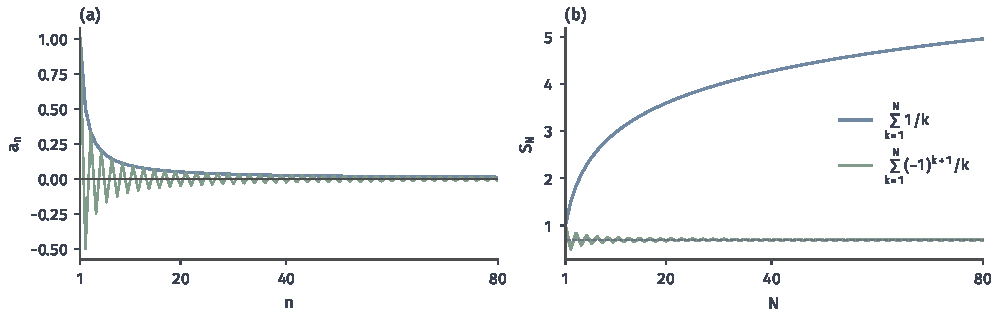
\includegraphics[width=169.0mm]{figures/01-mathematical-preliminaries-upper/00-shared/matplotlib/chapter3-concept-processes/series-terms-sums.pdf}
 \caption{(a) 蓝、绿折线分别连接$1/n$与$(-1)^{n+1}/n$的前80项。(b) 对应的部分和：调和部分和继续增长，交错调和部分和趋于虚线所示的$\log2$。项趋零只是级数收敛的必要条件；图展示有限段，收敛或发散由正文中的判别证明。}
 \label{fig:analysis-process-series-terms-sums}
\end{figure*}

\paragraph{Dirichlet判别}
交错级数的论证可以推广：若一列数的部分和有界振荡，再配上单调趋零的权重，乘积级数仍收敛。这一推广称为Dirichlet判别，作为补充推导列在这里，第~\ref{sec:ru-power-series-uniform}节证明幂级数在端点附近的一致收敛时要用到同样的技巧。

设$A_N=\sum_{n=1}^Na_n$满足$|A_N|\leq M$，$b_n\geq0$单调趋零。对$m\leq k$记$A^{(m)}_k=\sum_{n=m}^ka_n$，则$|A^{(m)}_k|\leq2M$，约定$A^{(m)}_{m-1}=0$。
把$a_k=A^{(m)}_k-A^{(m)}_{k-1}$代入有限和并重新组合（称为有限分部求和），得到
\[
 \sum_{k=m}^Na_kb_k=A^{(m)}_Nb_N+\sum_{k=m}^{N-1}A^{(m)}_k(b_k-b_{k+1}).
\]
由于$b_k-b_{k+1}\geq0$，右侧绝对值不超过$2M\bigl[b_N+\sum_{k=m}^{N-1}(b_k-b_{k+1})\bigr]=2Mb_m$，它与$N$无关且随$m$增大趋于零，由柯西准则知$\sum a_nb_n$收敛。
取$a_n=(-1)^{n+1}$便回到交错情形。

\subsection{级数的重排与分组对收敛的影响}
\label{sec:ru-series-rearrangement-grouping}
\label{sec:analysis-series-rearrangement-grouping}

有限和可以任意交换项的先后、任意加括号。无穷级数的和是部分和的极限，改变次序或加括号会改变部分和数列，因而需要重新检验。
重排改变各项进入累计的顺序，分组只把原次序中有限个相邻项合并，两种操作的效果不同。

\paragraph{级数的重排}
若$\pi:\{1,2,\ldots\}\to\{1,2,\ldots\}$为双射，级数$\sum_na_{\pi(n)}$称为原级数的\term{重排}（rearrangement），它恰好使用每一项一次。
\begin{theorem}[保持和的重排]
\label{thm:ru-rearrangement}
非负项级数的任意重排与原级数有相同的扩展总和；绝对收敛级数的任意重排仍收敛，并且和不变。
\end{theorem}
\begin{proof}
对非负项，重排的每个部分和只含有限个原下标，它们都不超过某个$N$，所以该部分和不超过$s_N$，从而不超过原扩展总和；反过来，原来的前$N$项也全部出现在重排的某个有限前段中。两个方向分别取上确界即得。

设原级数绝对收敛，和为$s$，记重排的部分和为$t_K$。给定$\varepsilon>0$，先选$N$使$\sum_{n>N}|a_n|<\varepsilon$，再选$K_0$使$\pi(1),\ldots,\pi(K_0)$已经包含$1,\ldots,N$。
当$K\geq K_0$时，$t_K-s_N$是若干个下标大于$N$的项之和，故$|t_K-s_N|<\varepsilon$；又$|s_N-s|<\varepsilon$，所以$|t_K-s|<2\varepsilon$。
\end{proof}

条件收敛没有这一保证。记前$N$项中正项之和为$P_N$、负项绝对值之和为$Q_N$。若二者的极限有一个有限，由$s_N=P_N-Q_N$收敛可知另一个也有限，
于是$\sum|a_n|$有限，与条件收敛矛盾；所以正项与负项的总和都是$+\infty$。

对任意目标$L$，按原相对次序取正项直到部分和超过$L$，再取负项直到低于$L$，如此反复；若原级数含有零项，每轮再插入一个尚未使用的零项。
正负项的总和都无限，每一轮都在有限步内结束，所有项最终都被用到；而$a_n\to0$使每次越过$L$的幅度趋于零，因此这个重排的和为$L$。
可见条件收敛级数的和依赖抵消的顺序，不能按有限和的交换律任意调换。

\paragraph{级数的分组}
分组保持原项的顺序，只把相邻项合为一项。取$0=n_0<n_1<n_2<\cdots$，令$c_j=\sum_{k=n_{j-1}+1}^{n_j}a_k$，则分组后前$J$项的和恰为$s_{n_J}$，是原部分和的子列。
所以原级数收敛到$s$时，分组后的级数也收敛到$s$，绝对收敛与条件收敛都是如此。
反向不成立：$1-1+1-1+\cdots$的部分和在$1$与$0$之间交替，原级数发散，
按$(1-1)+(1-1)+\cdots$分组后各项却都为零。分组只保留部分截断位置，可能掩盖块内的振荡。

非负项没有这种抵消：原部分和单调，分组截断又越过每一个原截断位置，两者的上确界相同，所以非负项级数可以任意保序分组，即使总和为$+\infty$。

\section{函数的极限}
\label{sec:ru-function-limits}
\label{sec:analysis-function-limits}

数列的下标按自然数逐项增加，函数的输入却可以从许多实数位置靠近同一点。例如$(x^2-1)/(x-1)$在$x=1$没有定义，但$x\neq1$时它等于$x+1$，邻近输入的输出仍趋于$2$。
函数极限研究的正是这种去掉中心点后的共同趋近，不要求函数在中心有取值。本节先给出定义和几种变形，再借数列极限建立存在性判别和运算法则，最后求出指数函数与三角函数在原点附近的基本极限。

\subsection{函数极限的定义、无穷小与无穷大}
\label{sec:ru-function-limit-definition}

讨论$x$靠近$a$，要先说清哪些点算靠近。以$a$为中心、半径为$r$的开区间$(a-r,a+r)$称为$a$的一个邻域，去掉中心后的$(a-r,a)\cup(a,a+r)$称为去心邻域。

还须保证定义域中确实有不同于$a$的点能够任意靠近$a$。设$X\subseteq\mathbb R$，若$a$的每个去心邻域都含有$X$中的点，就称$a$为$X$的\term{聚点}（cluster point）；
$a$本身可以不属于$X$，例如$0$是$(0,1)$的聚点。$X$中不是聚点的点称为\term{孤立点}（isolated point），例如整数集合中的每个点：附近没有其他输入，谈不上趋近。

\begin{definition}[函数的极限]
\label{def:ru-function-limit}
设$f:X\to\mathbb R$，$a$为$X$的聚点，$b\in\mathbb R$。若对每个$\varepsilon>0$，都存在$\delta>0$，使
\[
 x\in X,\quad0<|x-a|<\delta\quad\Longrightarrow\quad|f(x)-b|<\varepsilon,
\]
就称$x\to a$时$f(x)$的极限为$b$，记作$\lim_{x\to a}f(x)=b$或$f(x)\to b$（$x\to a$）。
\end{definition}
这里用输入误差$\delta$控制输出误差$\varepsilon$，与数列用尾部起点控制误差的思路相同。条件$0<|x-a|$排除了中心点，所以既不要求$f(a)$有定义，也不要求它等于$b$。
回到开头的例子：$x\neq1$时$f(x)=x+1$，给定$\varepsilon>0$取$\delta=\varepsilon$，则$0<|x-1|<\delta$时$|f(x)-2|=|x-1|<\varepsilon$，所以极限为$2$。

图~\ref{fig:analysis-process-epsilon-delta-band}把输入邻域与输出误差带对应起来，并把中心处的函数值与极限分开。

\begin{figure}[!htbp]
 \centering
 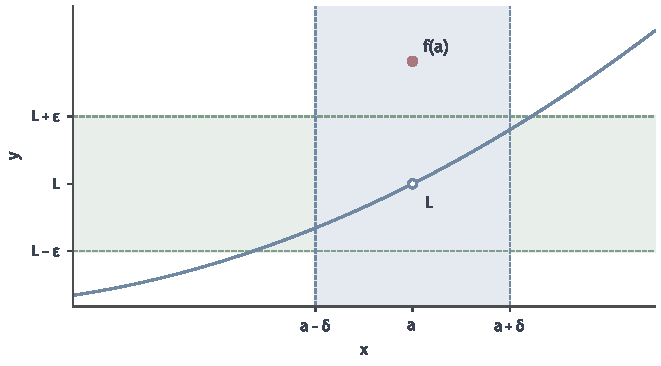
\includegraphics[width=112.0mm]{figures/01-mathematical-preliminaries-upper/00-shared/matplotlib/chapter3-concept-processes/epsilon-delta-band.pdf}
 \caption{取$a=L=1$（$L$即正文中的极限值$b$），$x\neq1$时$f(x)=x^2$，另令$f(1)=2$。蓝带对应$\delta=0.2$的输入范围，绿带对应$\varepsilon=0.55$的输出范围；去掉$a$后，蓝带内曲线全部落在绿带内。空心点是极限位置，红实心点是$f(a)$，不参加去心邻域条件。}
 \label{fig:analysis-process-epsilon-delta-band}
\end{figure}

\paragraph{单侧极限与无穷处的极限}
实轴上的输入可以从两侧接近一点，两侧的输出未必有相同趋向。只让$x<a$的输入趋近$a$，得到左极限$\lim_{x\to a^-}f(x)$；只让$x>a$的输入趋近，得到右极限$\lim_{x\to a^+}f(x)$。
两者分别在上述条件中加上$x<a$或$x>a$，并要求那一侧有定义域中的点任意靠近$a$。两侧都能趋近时，极限存在当且仅当左右极限都存在且相等。

例如阶跃函数$\mathbb I\{x\geq0\}$在$0$处的左极限为$0$、右极限为$1$，所以极限不存在。在闭区间$[a,b]$上，左端点只能从右侧趋近，右端点只能从左侧趋近，端点处的极限总是指单侧极限。

输入还可以趋向无穷。设定义域向右无界，$\lim_{x\to+\infty}f(x)=b$表示：对每个$\varepsilon>0$，存在$M$使定义域中所有$x>M$都满足$|f(x)-b|<\varepsilon$；$x\to-\infty$类似。

输出也可以越过任何有限界：对有限聚点$a$，$f(x)\to+\infty$（$x\to a$）表示对每个实数$M$都存在$\delta>0$，使定义域中满足$0<|x-a|<\delta$的$x$都有$f(x)>M$。
以$1/x$为例：$x\to\pm\infty$时它趋于$0$，这是输入趋向无穷；$x\to0^+$时它趋于$+\infty$，$x\to0^-$时趋于$-\infty$，这是输出趋向无穷，两侧方向不同，因而没有共同的双侧极限。

\paragraph{无穷小、无穷大与渐近记号}
\label{sec:comb-growth-scales}
趋向零的量出现在误差、余项和微分中，需要一个统一的名称。在指定的趋向下极限为$0$的函数或数列称为\term{无穷小}（infinitesimal），绝对值趋于$+\infty$的称为无穷大。

例如$x\to0$时$x$与$x^2$都是无穷小，$n\to\infty$时$1/n$是无穷小。无穷小描述的是一个变化过程的极限性质，不是某个固定的很小的数。若$f$在趋向附近非零，则$f$为无穷大当且仅当$1/f$为无穷小。

两个无穷小趋于零的相对速度可以不同，比较它们的比值即可。设在所讨论的趋向附近$g\neq0$。
\begin{definition}[渐近记号]
\label{def:ru-asymptotic-notation}
若$f/g\to0$，记$f=o(g)$，表示$f$相对于$g$可以忽略；若$|f/g|$在趋向附近有界，即存在常数$C$使最终$|f|\leq C|g|$，记$f=O(g)$；若$f/g\to1$，记$f\sim g$，称二者等价。
\end{definition}
例如$x\to0$时$x^2=o(x)$，$3x=O(x)$但不是$o(x)$，$x+x^2\sim x$。比值把这些记号与相对误差联系起来：$f\sim g$恰好说明用$g$近似$f$的相对误差$|f-g|/|g|$趋于零。

等价无穷小可以在乘除中互相替换：若$f\sim f_1$、$g\sim g_1$，则$fg/(f_1g_1)=(f/f_1)(g/g_1)\to1$。相减时却不行，因为主要部分可能相互抵消。
例如$x\to0$时$f(x)=x+x^2$与$g(x)=x$都等价于$x$，若把两者都换成$x$再相减会得到$0$，而实际上$f-g=x^2$。抵消以后，留下的是原先被忽略的高阶部分，必须保留更精细的展开才能判断。

同样的记号可用于$n\to\infty$的数列，用来比较增长的快慢。$3n+7=O(n)$、$n/10=O(n)$，但两个比值分别趋于$3$和$0.1$，都不是$o(n)$；$10\sqrt n=o(n)$，因为$10\sqrt n/n\to0$。

对最终为正的数列，若存在$c>0$使$a_n\geq cb_n$最终成立，记$a_n=\Omega(b_n)$；同时满足$O$与$\Omega$时记$a_n=\Theta(b_n)$，表示同一数量级。
$n=O(n^2)$也成立，所以大$O$只给出上界，不一定是精确的增长阶。后文描述算法的计算量时沿用这里的含义，比较的始终是两个数量的比值。
图~\ref{fig:vol1-add-asymptotic-ratios}画出了上面三个比值。

\begin{figure}[!htb]
 \centering
 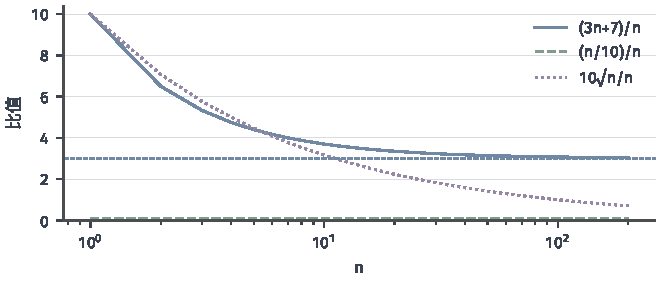
\includegraphics[width=112mm]{figures/01-mathematical-preliminaries-upper/00-shared/matplotlib/mathematical-language-combinatorics-analysis-optimization-comprehension-additions/asymptotic-ratios.pdf}
 \caption{三个解析数列除以$n$后的比值，展示整数$n=1,\ldots,200$，横轴为对数刻度。蓝、绿、紫线的极限分别为$3,0.1,0$。前两者对应$O(n)$而非$o(n)$，第三者对应$o(n)$；极限由正文中的表达式判断，有限范围曲线只帮助观察。}
 \label{fig:vol1-add-asymptotic-ratios}
\end{figure}

\subsection{函数极限存在的判别}
\label{sec:ru-function-limit-criteria}

函数极限要求控制$a$附近所有允许的输入，直接验证并不方便。下面的序列判据把它转化为数列极限，使上一节的工具可以直接使用。
\begin{theorem}[函数极限的序列判据]
\label{thm:ru-sequential-criterion}
设$a$为$X$的聚点。$\lim_{x\to a}f(x)=b$，当且仅当对每个满足$x_n\in X\setminus\{a\}$且$x_n\to a$的数列，都有$f(x_n)\to b$。
\end{theorem}
\begin{proof}
设函数极限为$b$。给定$\varepsilon$取相应的$\delta$，充分靠后的$x_n$满足$0<|x_n-a|<\delta$，于是$|f(x_n)-b|<\varepsilon$。

反过来用反证法。若误差条件不成立，就存在$\varepsilon_0>0$，使每个$\delta=1/n$都不合要求，即可选$x_n\in X$满足$0<|x_n-a|<1/n$而$|f(x_n)-b|\geq\varepsilon_0$；这列输入趋于$a$，输出却不趋于$b$。
\end{proof}
序列判据也是否定极限存在的常用工具：只要找到两列趋于$a$的输入，使输出趋于不同的值。例如$f(x)=\sin(1/x)$，沿$x_n=1/(2n\pi+\pi/2)$恒有$f(x_n)=1$，沿$y_n=1/(2n\pi+3\pi/2)$恒有$f(y_n)=-1$，所以$x\to0$时极限不存在。

不知道候选极限时，也可以像数列那样检查输出是否彼此接近。
\begin{theorem}[函数极限的柯西准则]
\label{thm:ru-function-cauchy}
设$a$为$X$的聚点。$x\to a$时$f(x)$有有限极限，当且仅当对每个$\varepsilon>0$，都存在$\delta>0$，使任意两个满足$0<|x-a|<\delta$、$0<|y-a|<\delta$的$x,y\in X$都有$|f(x)-f(y)|<\varepsilon$。
\end{theorem}
\begin{proof}
必要性由三角不等式得到：两个输出都与极限相差不到$\varepsilon/2$。

充分性先固定一列$x_n\in X\setminus\{a\}$、$x_n\to a$。对给定的$\varepsilon$，充分靠后的$x_n,x_m$都落在$\delta$去心邻域内，所以$(f(x_n))$是柯西数列，由实数的完备性收敛到某个$b$。
另取一列$y_n\to a$，把两列交错排成$x_1,y_1,x_2,y_2,\ldots$，它仍趋于$a$，输出列同样收敛；它的两个子列$(f(x_n))$与$(f(y_n))$必有同一极限。
所以每列趋于$a$的输入都给出同一个$b$，由序列判据，$f(x)\to b$。
\end{proof}
准则中的两个输入都不等于$a$，这与极限只看去心邻域的约定一致。数列的柯西准则依赖确界原理，这里通过它同样依赖实数的完备性。

\paragraph{极限的运算法则}
借助序列判据，数列极限的运算法则可以逐条搬到函数上。
\begin{theorem}[函数极限的运算法则]
\label{thm:ru-function-limit-laws}
设$a$为$X$的聚点，$f,g:X\to\mathbb R$，$x\to a$时$f(x)\to b$、$g(x)\to c$，其中$b,c\in\mathbb R$，$\lambda$为实常数，则$x\to a$时
\begin{enumerate}
 \item 和与差：$f(x)\pm g(x)\to b\pm c$；
 \item 数乘：$\lambda f(x)\to\lambda b$；
 \item 积：$f(x)g(x)\to bc$；
 \item 商：若$c\neq0$，则在$a$的某个去心邻域内$g\neq0$，并且$f(x)/g(x)\to b/c$。
\end{enumerate}
\end{theorem}
\begin{proof}
任取$x_n\in X\setminus\{a\}$、$x_n\to a$，由序列判据，$f(x_n)\to b$、$g(x_n)\to c$。对这两列数分别使用定理~\ref{thm:ru-sequence-limit-laws}中的和、差、数乘与积的法则，再由序列判据返回函数极限，即得前三条。

对商，先在$g$的极限定义中取$\varepsilon=|c|/2$，得到一个去心邻域，其中$|g(x)|>|c|/2>0$；在这个邻域内任取趋于$a$的输入列，用数列的商法则，再由序列判据返回。
\end{proof}
分子分母都趋于零时不能套用商的法则。例如$(x^2-1)/(x-1)$在$x\to1$时须先约去公因子$x-1$，才能求出极限$2$。

\begin{theorem}[函数极限的夹逼定理]
\label{thm:ru-function-squeeze}
若在$a$的某个去心邻域内，所有允许的输入都满足$u(x)\leq h(x)\leq v(x)$，且$x\to a$时$u(x)\to L$、$v(x)\to L$，其中$L\in\mathbb R$，则$h(x)\to L$。
\end{theorem}
\begin{proof}
任给$\varepsilon>0$，取一个共同的去心邻域，使其中$u(x)$与$v(x)$都落在$(L-\varepsilon,L+\varepsilon)$内，夹在中间的$h(x)$也在其中。
\end{proof}
例如$-|x|\leq x\sin(1/x)\leq|x|$，所以$x\to0$时$x\sin(1/x)\to0$。

复合函数的极限需要多一点小心。设$x\to a$时$f(x)\to b$，$y\to b$时$g(y)\to c$。若在$a$的某个去心邻域内$f(x)\neq b$，或者$g$在$b$处有定义且$g(b)=c$，则$g(f(x))\to c$。

没有这两个条件之一，结论可能失败：令$f\equiv b$为常数，$g(y)=1$（$y\neq b$）、$g(b)=0$，则$y\to b$时$g(y)\to1$，但$g(f(x))\equiv0$。
问题在于外层的极限只看$b$的去心邻域，而内层的输出可能恰好落在被排除的$b$上；第一个条件保证这种情形不发生，第二个条件则说明即使发生也没有影响。

\subsection{基本函数的极限}
\label{sec:ru-elementary-limits}

上一章把指数和三角函数当作已知对象。现在有了级数和函数极限，可以给出指数函数的定义，并求出后面计算导数要用的两个基本极限。

\paragraph{自然指数函数}
对每个实数$x$，级数$\sum_{k\geq0}x^k/k!$相邻项绝对值之比为$|x|/(k+1)\to0$，由比值判别绝对收敛。定义
\[
 \exp x=\sum_{k=0}^\infty\frac{x^k}{k!}.
\]

指数函数最重要的性质是加法公式$\exp(x+y)=\exp x\,\exp y$。证明要计算两个级数的乘积，先说明绝对收敛级数可以按总次数归并。

设$\sum_ka_k$与$\sum_jb_j$绝对收敛。有限的正方形和满足$\sum_{k,j\leq N}a_kb_j=(\sum_{k\leq N}a_k)(\sum_{j\leq N}b_j)$，因此趋于两个和的乘积。
按总次数$k+j=n\leq N$归并的三角形和，与正方形和只差满足$k,j\leq N$、$k+j>N$的项；这些项中$k$或$j$大于$N/2$，其绝对值之和不超过
$(\sum_{k>N/2}|a_k|)(\sum_j|b_j|)+(\sum_k|a_k|)(\sum_{j>N/2}|b_j|)$，它随$N$增大趋于零。所以按总次数归并后得到同一极限。

用于指数级数，第$n$组为$\sum_{k=0}^nx^ky^{n-k}/[k!(n-k)!]$，由二项式定理它等于$(x+y)^n/n!$，于是
\[
 \exp x\,\exp y=\sum_{n=0}^\infty\frac{(x+y)^n}{n!}=\exp(x+y).
\]
记$e=\exp1\approx2.71828$。由加法公式，对正整数$n$有$\exp n=e^n$，因此通常把$\exp x$写作$e^x$。

加法公式推出了上一章当作已知的几条性质。由$e^xe^{-x}=e^0=1$知$e^x\neq0$，又$e^x=(e^{x/2})^2\geq0$，所以$e^x>0$。
对$u\geq0$，级数各项非负，只保留前两项便得$e^u\geq1+u$；于是$h>0$时$e^{x+h}=e^xe^h\geq e^x(1+h)>e^x$，指数函数严格递增。
同一不等式说明$x\to+\infty$时$e^x\to+\infty$，再由$e^x=1/e^{-x}$得$x\to-\infty$时$e^x\to0$。

原点附近的变化可以直接从级数估计。当$0<|h|<1/2$时，由$1/k!\leq1$，
\[
 |e^h-1-h|\leq\sum_{k=2}^\infty|h|^k=\frac{h^2}{1-|h|}\leq2h^2.
\]
除以$|h|$得$|(e^h-1)/h-1|\leq2|h|$，因此
\[
 \lim_{h\to0}\frac{e^h-1}{h}=1.
\]
这一推导只用到级数的估计，没有用到导数或逐项求导。同一估计还给出$|e^{x+h}-e^x|=e^x|e^h-1|\leq e^x(|h|+2h^2)\to0$，下一节将据此说明指数函数连续，并构造它的反函数自然对数。

\paragraph{三角函数的基本极限}
三角函数的基本极限来自单位圆上的几何比较。设$0<h<\pi/2$，比较单位圆中以$h$为圆心角的内接三角形、扇形与外切三角形的面积，得到$\sin h\leq h\leq\tan h$，即
\[
 \cos h\leq\frac{\sin h}h\leq1.
\]
又由$1-\cos h=2\sin^2(h/2)\leq h^2/2$，得到$0\leq1-\sin h/h\leq h^2/2$。$\sin h/h$是偶函数，同一估计对$h<0$也成立，由夹逼定理，
\[
 \lim_{h\to0}\frac{\sin h}h=1,\qquad\lim_{h\to0}\frac{\cos h-1}h=0,
\]
后者来自$|1-\cos h|/|h|\leq|h|/2$。第一个极限恰为$1$，依赖于用弧长度量角；若用角度制，会多出比例系数$\pi/180$。

\section{连续性}
\label{sec:ru-continuity}
\label{sec:analysis-local-models}
\label{sec:analysis-metric-continuity-extrema}

对$f(x)=x^2$，输入$x$接近$a$时，输出接近$a^2$，而$a^2$恰好是函数在$a$处的值。连续性描述的就是这种关系：输出趋近的目标等于函数在该点的取值。
本节先给出定义和运算性质，再研究闭区间上的连续函数为什么一定达到最值、取遍中间值，最后比较几种强弱不同的连续性条件。

\subsection{连续性的定义和性质}
\label{sec:ru-continuity-definition}

\begin{definition}[连续]
\label{def:analysis-continuity}
设$X\subseteq\mathbb R$，$f:X\to\mathbb R$，$a\in X$。若对每个$\varepsilon>0$，都存在$\delta>0$，使
\[
 x\in X,\quad|x-a|<\delta\quad\Longrightarrow\quad|f(x)-f(a)|<\varepsilon,
\]
则称$f$在$a$处\term{连续}（continuous）。若$f$在$X$的每一点连续，就称$f$为连续函数。
\end{definition}
与函数极限的定义相比，这里不排除$x=a$，因为目标值就是$f(a)$。连续性与极限的关系取决于$a$在定义域中的位置。
若$a$是$X$的聚点，连续等价于$\lim_{x\to a}f(x)=f(a)$；若$a$是孤立点，取$\delta$足够小，使邻域内属于$X$的点只有$a$，条件自动成立；
若$a$是闭区间的端点，连续就是相应的单侧极限等于函数值。

用定义验证连续性时，需要对每个$\varepsilon$具体找出$\delta$。
\begin{example}[平方函数在每一点连续]
\label{ex:analysis-square-pointwise-continuity}
设$f(x)=x^2$，固定$a$。若$|x-a|<1$，则$|x+a|\leq|x-a|+2|a|<2|a|+1$，从而$|x^2-a^2|=|x-a|\,|x+a|\leq(2|a|+1)|x-a|$。
给定$\varepsilon>0$，取$\delta=\min\{1,\varepsilon/(2|a|+1)\}$，则$|x-a|<\delta$时$|x^2-a^2|<\varepsilon$。
\end{example}
例中的$\delta$随$|a|$增大而缩小：基点离原点越远，图像越陡，允许的输入误差越小。第~\ref{sec:analysis-continuity-relations}节将说明，在整条实轴上这种依赖无法消除。

不连续的点称为间断点，按失效方式可以分为几类。若$\lim_{x\to a}f(x)$存在但不等于$f(a)$，称为可去间断：改变$f(a)$的值，函数便连续，例如把$x^2$在$0$处的值改为$1$。
若左右极限都存在但不相等，称为跳跃间断，例如阶跃函数$\mathbb I\{x\geq0\}$在$0$处。两类并未穷尽所有情形：令$f(0)=0$、$x\neq0$时$f(x)=\sin(1/x)$，上一节已看到它在$0$处连单侧极限都不存在，这是振荡导致的间断。

连续性可以用序列刻画：$f$在$a\in X$处连续，当且仅当对每列满足$x_n\in X$、$x_n\to a$的输入，都有$f(x_n)\to f(a)$。证明与函数极限的序列判据相同，只是不必排除$x_n=a$。
由此，函数极限的运算法则直接给出：$f,g$在$a$处连续时，$f\pm g$、$fg$、$cf$在$a$处连续；若还有$g(a)\neq0$，则$f/g$在$a$附近有定义并在$a$处连续。
复合同样保持连续：若$f$在$a$处连续，$g$在$f(a)$处连续，则$g\circ f$在$a$处连续。给定$\varepsilon$，先由$g$的连续性得到$\eta$，再由$f$的连续性取$\delta$使$|f(x)-f(a)|<\eta$，两步误差传递便连成一步。
与复合函数的极限不同，这里外层在$f(a)$处连续，所以不需要额外条件。由这些规则，多项式在$\mathbb R$上连续，有理函数在分母非零处连续。
本节只用实轴上的绝对值距离；把输入和输出的距离换成一般的度量，就得到第~\ref{chap:metric-spaces}章中一般映射的连续性。

\subsection{闭区间上连续函数的性质}
\label{sec:ru-closed-interval-continuity}
\label{sec:analysis-metric-measurement}
\label{sec:analysis-set-metric}

函数$f(x)=x$在$(0,1)$上连续，却没有最小值；在$[0,1]$上则有。区别来自定义域：$(0,1)$中的点列$1/n$趋于$0$，极限却不在定义域内。
要从各点的局部性质得到整个定义域上的结论，需要先描述哪些集合能留住其中点列的极限，以及怎样把局部控制合成整体控制。

集合$U\subseteq\mathbb R$若对每个$x\in U$都存在$r>0$使$(x-r,x+r)\subseteq U$，就称为\term{开集}（open set）；补集为开集的集合称为\term{闭集}（closed set）。
开区间是开集，闭区间是闭集；$[0,1)$既不开也不闭，$\mathbb R$与空集既开又闭。闭集的意义可以换成点列的语言来理解。
\begin{lemma}[闭集的序列判据]
\label{lem:analysis-closed-sequence-criterion}
$F\subseteq\mathbb R$是闭集，当且仅当：每个取值于$F$的收敛数列，其极限也属于$F$。
\end{lemma}
\begin{proof}
设$F$闭。若取值于$F$的数列收敛到$x\notin F$，开集$\mathbb R\setminus F$包含某个$(x-r,x+r)$，充分靠后的项都落在其中，与$x_n\in F$矛盾。
反之，若$F$不闭，补集不是开集，存在$x\notin F$使每个$(x-1/n,x+1/n)$都与$F$相交；从中各选一点$x_n\in F$，则$x_n\to x\notin F$。
\end{proof}
闭与有界是不同的性质：$(0,1)$有界但不闭，$\mathbb R$闭但无界。二者同时成立时，Bolzano--Weierstrass定理给出收敛子列，本引理又保证子列的极限仍在集合内。
这一“闭有界集中的点列有收敛到集合内的子列”的性质，是本小节各定理的共同依据。

同一性质还有另一种表达：把局部控制合成整体控制。若一族开集的并包含$K$，称它们为$K$的\term{开覆盖}（open cover）；若能从中选出有限个仍覆盖$K$，称为\term{有限子覆盖}（finite subcover）。
若$K$的每个开覆盖都有有限子覆盖，称$K$\term{紧致}（compact）。
\begin{theorem}[闭区间的有限子覆盖性质]
\label{thm:analysis-interval-finite-subcover}
实轴上的每个闭区间$[a,b]$都是紧致集。
\end{theorem}
\begin{proof}
设$a<b$，给定$[a,b]$的开覆盖$\mathcal U$。先证明存在一个共同尺度：
\begin{equation}
 \exists r>0,\quad\forall x\in[a,b],\quad\exists U\in\mathcal U,\qquad(x-r,x+r)\cap[a,b]\subseteq U.
 \label{eq:analysis-cover-uniform-radius}
\end{equation}
若不然，对每个$n$可选$x_n\in[a,b]$，使$(x_n-1/n,x_n+1/n)\cap[a,b]$不包含于任何覆盖成员。取收敛子列$x_{n_k}\to x\in[a,b]$，选$U\in\mathcal U$与$\rho>0$使$(x-\rho,x+\rho)\subseteq U$。
当$k$足够大时$|x_{n_k}-x|<\rho/2$且$1/n_k<\rho/2$，于是$(x_{n_k}-1/n_k,x_{n_k}+1/n_k)\subseteq U$，与选取矛盾。
有了共同半径$r$，把$[a,b]$分成有限个长度小于$r$的小段，每段落在某个$(x-r,x+r)$内，因而被一个覆盖成员包含；每段选一个成员即得有限子覆盖。
\end{proof}
图~\ref{fig:analysis-process-finite-open-cover}对照闭区间的有限覆盖与开区间上无法有限选取的覆盖。每个有界闭集也是紧致的：把它放进某个$[a,b]$，把它的补集加入开覆盖，应用定理后再删去补集即可。
有限子覆盖与收敛子列是同一性质的两种说法，后者在下面的证明中更直接，前者在需要把无限多个局部估计合成一个时更方便。

\begin{figure}[!htbp]
 \centering
 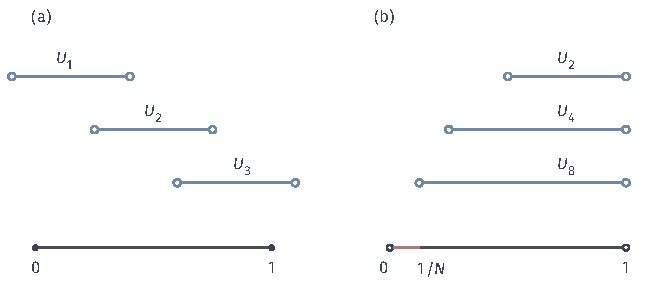
\includegraphics[width=112mm]{figures/01-mathematical-preliminaries-upper/00-shared/tikz/chapter3-concept-processes/finite-open-cover.pdf}
 \caption{(a) 三个开区间$(-0.1,0.4)$、$(0.25,0.75)$、$(0.6,1.1)$覆盖$[0,1]$。(b) $U_n=(1/n,1)$（$n\geq2$）覆盖$(0,1)$；只选有限多个时，设最大下标为$N$，红段$(0,1/N]$仍未覆盖。图只画$U_2,U_4,U_8$；右侧的失败由最大下标论证，不是有限图像的猜测。}
 \label{fig:analysis-process-finite-open-cover}
\end{figure}

\begin{theorem}[极值定理]
\label{thm:analysis-extreme-value}
设$K\subseteq\mathbb R$非空、闭且有界，$f:K\to\mathbb R$连续，则$f$有界，并在$K$上达到最小值和最大值。
\end{theorem}
\begin{proof}
若$f$无界，可选$x_n\in K$使$|f(x_n)|>n$；取收敛子列$x_{n_k}\to x\in K$，连续性给出$f(x_{n_k})\to f(x)$，收敛数列有界，与$|f(x_{n_k})|>n_k$矛盾。
于是$m=\inf_Kf$是有限实数。对每个$n$选$x_n\in K$使$m\leq f(x_n)<m+1/n$，取收敛子列$x_{n_k}\to x^\star\in K$，则$f(x_{n_k})\to f(x^\star)$，同时$f(x_{n_k})\to m$，所以$f(x^\star)=m$。对$-f$重复论证即得最大值。
\end{proof}
三个条件各排除一种失效方式：有界保证收敛子列，闭保证子列的极限仍在定义域内，连续保证函数值随之收敛。下面三个例子各缺一个条件，下确界都取不到。
\begin{example}[极值定理的条件]
\label{ex:analysis-extrema-failures}
定义域不闭：$f(x)=x$在$(0,1)$上的下确界$0$不被取得。定义域无界：$e^x$在$\mathbb R$上连续，下确界为$0$，但$e^x>0$，取不到。
函数不连续：在$[0,1]$上令$f(0)=1$、$x>0$时$f(x)=x$，下确界为$0$，而$f$在每一点的值都大于$0$。
\end{example}

另一条整体性质说的是：函数从一个值变到另一个值时，要经过中间的每个值。这要求两端之间的整段都属于定义域。
\begin{theorem}[介值定理]
\label{thm:analysis-intermediate-value}
设$a<b$，$f:[a,b]\to\mathbb R$连续。则对介于$f(a)$与$f(b)$之间的每个$c$，都存在$\xi\in[a,b]$使$f(\xi)=c$；若$c$严格位于二者之间，可取$\xi\in(a,b)$。
\end{theorem}
\begin{proof}
设$f(a)<c<f(b)$（端点值相等的情形直接取端点，$f(a)>f(b)$时考虑$-f$）。令$S=\{x\in[a,b]:f(x)\leq c\}$，它含$a$且以$b$为上界，由确界原理$u=\sup S$存在。
取$x_n\in S$使$x_n\to u$，连续性给出$f(u)\leq c$，因而$u\neq b$。若$f(u)<c$，由连续性，$u$右侧充分近的点仍满足$f<c$，它们属于$S$却大于$u$，矛盾。所以$f(u)=c$，又由$f(a)<c$知$u\neq a$。
\end{proof}
证明用到了区间不缺中间点：确界$u$仍在区间中，并且$u$的右侧还有区间内的点。定义域闭且有界但有缺口时，介值性可能失效。
\begin{example}[有缺口的定义域上不取中间值]
\label{ex:analysis-intermediate-value-gap}
令$X=[-2,-1]\cup[1,2]$，在$[-2,-1]$上取$f=0$，在$[1,2]$上取$f=1$。对每个$a\in X$取$\delta=1$，邻域内属于$X$的点与$a$在同一段，所以$f$连续。$X$闭且有界，$f$却不取$1/2$。
\end{example}
这个函数在$X$上仍然达到最值：闭有界足以保证最值，却不能代替介值定理的区间条件。

介值定理最直接的用途是证明方程有解。若$f$在$[a,b]$上连续且$f(a)f(b)<0$，则$f$在$(a,b)$内有零点。这个结论还给出求零点的方法，即\term{二分法}（bisection method）：
取中点$m=(a+b)/2$，若$f(m)=0$则停止，否则保留端点函数值异号的那一半，重复进行。$n$步后零点落在长度为$(b-a)/2^n$的区间内，取该区间中点作为近似值，误差不超过$(b-a)/2^{n+1}$。
例如$f(x)=x^2-2$在$[1,2]$上两端异号，第一步$f(1.5)=0.25>0$保留$[1,1.5]$，第二步$f(1.25)<0$保留$[1.25,1.5]$；要使误差小于$10^{-6}$，约需$20$步。
二分法只用到连续性和符号，不需要导数；所需步数由误差界事先确定。

介值定理还说明，区间上的连续函数把区间映成区间：若$f(I)$中有$y_1<y_2$，它们之间的每个值也被取到。由此可以研究反函数的连续性。
\begin{theorem}[严格单调连续函数的反函数]
\label{thm:ru-inverse-continuity}
\label{sec:analysis-inverse-continuity}
设$f$在区间$I$上连续且严格单调，则$f(I)$是区间，$f:I\to f(I)$是双射，并且反函数$f^{-1}$在$f(I)$上连续、与$f$同向严格单调。
\end{theorem}
\begin{proof}
双射与单调性已在第~\ref{sec:ru-function-properties}节说明，$f(I)$是区间由介值定理得到。以严格递增、$a$为$I$的内点为例，给定足够小的$\varepsilon>0$使$a\pm\varepsilon\in I$，有$f(a-\varepsilon)<f(a)<f(a+\varepsilon)$。
取$\delta=\min\{f(a)-f(a-\varepsilon),\,f(a+\varepsilon)-f(a)\}$，若$y\in f(I)$且$|y-f(a)|<\delta$，则$f(a-\varepsilon)<y<f(a+\varepsilon)$，严格递增迫使$f^{-1}(y)\in(a-\varepsilon,a+\varepsilon)$。端点只在一侧取点，论证相同。
\end{proof}

现在可以严格构造自然对数。上一节已经得到：$e^x$严格递增，$x\to-\infty$时趋于$0$，$x\to+\infty$时趋于$+\infty$，并且$|e^{x+h}-e^x|\leq e^x(|h|+2h^2)$，所以它在每一点连续。
对任意$y>0$，先取两个输入使指数值分别小于和大于$y$，再用介值定理得到原像；严格单调保证原像唯一。所以$e^x$是$\mathbb R$到$(0,+\infty)$的双射，它的反函数称为\term{自然对数}（natural logarithm），记作$\log x$，定义在$x>0$上。
由定理~\ref{thm:ru-inverse-continuity}，$\log$连续且严格递增；由指数的加法公式，$\log(xy)=\log x+\log y$。对$a>0$与实数$x$，定义$a^x=e^{x\log a}$，它对整数$x$与通常的乘幂一致。
这样，上一章作为背景使用的指数—对数关系，现在都有了依据。

\subsection{一致连续与Lipschitz连续}
\label{sec:ru-uniform-lipschitz}
\label{sec:analysis-continuity-relations}

连续性定义中的$\delta$可以随基点改变，平方函数的例子中$\delta$就随$|a|$增大而缩小。若要求同一个$\delta$适用于整个定义域，或者要求输出误差不超过输入误差的固定倍数，就得到更强的条件。
\begin{definition}[一致连续]
\label{def:analysis-uniform-continuity}
函数$f:X\to\mathbb R$称为\term{一致连续}（uniformly continuous），若对每个$\varepsilon>0$，都存在$\delta>0$，使任意$x,y\in X$满足$|x-y|<\delta$时都有$|f(x)-f(y)|<\varepsilon$。
\end{definition}
与逐点连续相比，变化在于量词的次序：逐点连续是“对每个点和每个$\varepsilon$，存在$\delta$”，一致连续是“对每个$\varepsilon$，存在对所有点都有效的$\delta$”。
\begin{example}[平方函数在实轴上不一致连续]
\label{ex:analysis-square-not-uniformly-continuous}
取$x_n=n$、$y_n=n+1/n$，则$|y_n-x_n|=1/n\to0$，而$y_n^2-x_n^2=2+1/n^2>2$。若平方函数在$\mathbb R$上一致连续，对$\varepsilon=1$取$\delta$，当$n>1/\delta$时便与上式矛盾。
\end{example}
两列点都逃向无穷远，那里平方函数越来越陡。把定义域限制在$[0,1]$上，则$|x^2-y^2|=|x+y|\,|x-y|\leq2|x-y|$，取$\delta=\varepsilon/2$即可。
同一个函数在两个定义域上表现不同，原因在于逃向无穷远的点列在有界闭集中不存在。
\begin{theorem}[一致连续性定理]
\label{thm:analysis-uniform-continuity}
设$K\subseteq\mathbb R$非空、闭且有界，$f:K\to\mathbb R$连续，则$f$在$K$上一致连续。特别地，闭区间上的连续函数一致连续。
\end{theorem}
\begin{proof}
若不然，存在$\varepsilon_0>0$，使每个$\delta=1/n$都对应$x_n,y_n\in K$，满足$|x_n-y_n|<1/n$而$|f(x_n)-f(y_n)|\geq\varepsilon_0$。
取收敛子列$x_{n_k}\to x\in K$，则$y_{n_k}\to x$。由$f$在$x$处连续，$f(x_{n_k})$与$f(y_{n_k})$都趋于$f(x)$，两者之差趋于零，与$\varepsilon_0$矛盾。
\end{proof}

一致连续只断言共同的$\delta$存在，没有给出输出误差与输入误差的数量关系。若这个关系是线性的，误差控制就更具体。
\begin{definition}[Lipschitz连续]
\label{def:analysis-lipschitz-continuity}
若存在常数$L\geq0$，使所有$x,y\in X$都满足
\begin{equation}
 |f(x)-f(y)|\leq L|x-y|,
 \label{eq:analysis-lipschitz-condition}
\end{equation}
则称$f$为\term{Lipschitz连续}（Lipschitz continuous）函数，$L$称为一个Lipschitz常数。若每一点都有一个邻域，$f$在其中满足这一条件（常数可随邻域改变），称$f$\term{局部Lipschitz连续}（locally Lipschitz）。
\end{definition}
Lipschitz连续蕴含一致连续：$L>0$时取$\delta=\varepsilon/L$即可。平方函数在$[0,1]$上可取$L=2$；在$\mathbb R$上割线斜率$x+y$无界，没有全局常数，
但在$(a-r,a+r)$内$|x+y|<2(|a|+r)$，所以它局部Lipschitz连续。

反过来，一致连续不蕴含Lipschitz连续。$\sqrt x$在$[0,1]$上连续，由一致连续性定理一致连续；但若有常数$L$，取$y=0$得$\sqrt x\leq Lx$，即$1/\sqrt x\leq L$对所有$x\in(0,1]$成立，这不可能。
它在零点附近的割线斜率无界。于是在同一个闭区间上有严格的强弱次序：Lipschitz连续强于一致连续，一致连续与连续等价；在无界区间上，连续又严格弱于一致连续。
比较时必须同时写明函数和定义域。控制许多短区间上总变化的绝对连续性，与积分能否恢复函数的问题相连，放在第~\ref{chap:measurable-functions}章讨论。

\section{函数列与函数项级数}
\label{sec:ru-function-sequences}

前几节的极限对象都是数。很多时候，我们用一系列函数逐步逼近同一个对象：几何级数的部分和$1+x+\cdots+x^N$逼近$1/(1-x)$，指数级数的部分和逼近$e^x$。
这时每个编号$n$对应一整个函数$f_n:X\to\mathbb R$，$(f_n)$称为\term{函数列}（sequence of functions）。
固定编号，看到的是一个函数；固定输入$x$，看到的是一列数$(f_n(x))_{n\geq1}$。函数列的收敛可以从后一个角度出发，但我们还关心收敛对整个函数意味着什么。

函数项级数$\sum_kg_k$的部分和$S_N=\sum_{k\leq N}g_k$本身就是一个函数列，级数的收敛与和函数都由部分和的极限决定。
所以下文先对函数列建立结论，再把它们用于部分和，不另建一套收敛语言。

\subsection{逐点收敛与一致收敛}
\label{sec:ru-pointwise-uniform}

最直接的做法是在每个输入处分别取数列极限。若对每个$x\in X$，数列$(f_n(x))$都收敛到$f(x)$，称$f_n$在$X$上\term{逐点收敛}（pointwise convergence）到$f$。
按数列极限的定义，这是说：对每个$x$和每个$\varepsilon>0$，存在$N$使$n\geq N$时$|f_n(x)-f(x)|<\varepsilon$，其中$N$可以随$x$改变。
若要求一个尾部起点同时控制全部输入，就得到更强的条件。
\begin{definition}[一致收敛]
\label{def:ru-uniform-convergence}
若对每个$\varepsilon>0$，都存在$N$，使$n\geq N$时对\emph{所有}$x\in X$都有$|f_n(x)-f(x)|<\varepsilon$，称$f_n$在$X$上\term{一致收敛}（uniform convergence）到$f$。
\end{definition}
两种收敛的差别与连续和一致连续的差别相同，都在于量词次序：$N$是否允许随$x$改变。

$f_n(x)=x^n$在$[0,1]$上的行为说明了这种差别。$0\leq x<1$时$x^n\to0$，$x=1$时恒为$1$，所以$f_n$逐点收敛到函数$f$，$f$在$[0,1)$上为$0$、在$1$处为$1$。
但在$x$接近$1$的地方，要使$x^n<1/2$，需要$n>\log2/\log(1/x)$，这个下界在$x\to1^-$时无界，没有一个$N$能同时管住所有$x$。
图~\ref{fig:ru-power-sequence-nonuniform}画出了几条$x^n$：无论$n$多大，曲线在靠近$1$处都要从接近$0$升到$1$，最大误差始终不小。

\begin{figure}[!htbp]
 \centering
 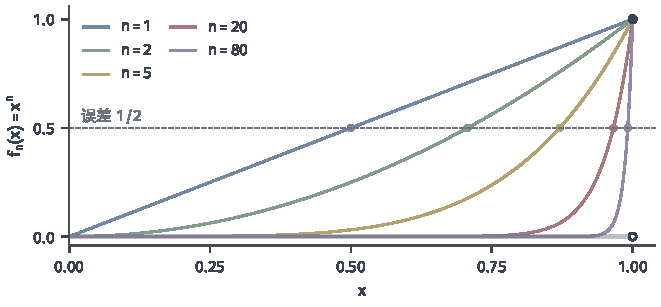
\includegraphics[width=112mm]{figures/01-mathematical-preliminaries-upper/02-real-numbers-and-univariate-functions/matplotlib/power-sequence-nonuniform/figure.pdf}
 \caption{函数列$f_n(x)=x^n$在$[0,1]$上的几条曲线（$n=1,2,5,20,80$）。逐点极限在$[0,1)$上为$0$（灰色水平线），在$x=1$处为$1$（实心点）。虚线标出误差$1/2$：每条曲线都在$x=2^{-1/n}$处越过它，越过位置随$n$增大逼近$1$，所以$\sup_{[0,1)}|f_n-f|=1$，收敛不一致。图为解析示例。}
 \label{fig:ru-power-sequence-nonuniform}
\end{figure}

\paragraph{一致收敛的判别}
直接检查一致收敛的办法是看最大误差。记$\|f_n-f\|_\infty=\sup_{x\in X}|f_n(x)-f(x)|$，则$f_n$一致收敛到$f$，当且仅当这个数列趋于零：两者说的都是“误差界可以对全部输入同时缩小”。
对$x^n$，在$[0,1)$上$\sup|x^n-0|=1$，不趋于零，所以收敛不一致；但在$[0,\rho]$（$\rho<1$）上，最大误差为$\rho^n\to0$，收敛是一致的。
可见一致收敛也依赖定义域，问题只出在$x=1$附近。这里的$\sup$只是一列数值的上确界，我们并没有把函数当作某个空间中的点。

不知道极限函数时，也可以用柯西条件检验。
\begin{theorem}[一致柯西准则]
\label{thm:ru-uniform-cauchy}
函数列$(f_n)$在$X$上一致收敛到某个函数，当且仅当对每个$\varepsilon>0$，存在$N$，使$m,n\geq N$时对所有$x\in X$都有$|f_m(x)-f_n(x)|<\varepsilon$。
\end{theorem}
\begin{proof}
必要性由三角不等式得到。对充分性，每个固定的$x$处$(f_n(x))$是柯西数列，因此收敛，记极限为$f(x)$。
在$|f_m(x)-f_n(x)|<\varepsilon$中固定$n\geq N$与$x$，令$m\to\infty$，得到$|f(x)-f_n(x)|\leq\varepsilon$，这个界对所有$x$同时成立。
\end{proof}

把一致柯西准则用于部分和，得到函数项级数最常用的判别法：用一列可求和的数值上界控制各项。
\begin{theorem}[Weierstrass判别法]
\label{thm:ru-weierstrass-m-test}
若存在非负数$M_k$，使$|g_k(x)|\leq M_k$对所有$x\in X$和$k$成立，且$\sum M_k<\infty$，则$\sum_kg_k$在$X$上一致收敛，并且对每个$x$绝对收敛。
\end{theorem}
\begin{proof}
对$m>n$，$|S_m(x)-S_n(x)|\leq\sum_{k=n+1}^m|g_k(x)|\leq\sum_{k>n}M_k$，右侧与$x$无关且随$n$增大趋于零，由一致柯西准则即得一致收敛；每个$x$处的绝对收敛由比较判别得到。
\end{proof}
例如$\sum_k\sin(kx)/k^2$在$\mathbb R$上一致收敛，可取$M_k=1/k^2$。第~\ref{sec:ru-power-series}节将用这一判别法证明幂级数在内部闭子区间上一致收敛。

\subsection{函数列连续性的保持}
\label{sec:ru-uniform-limit-continuity}

$x^n$的例子中，每个$f_n$都连续，逐点极限却在$1$处跳跃。所以逐点收敛不能保持连续性。一致收敛补上了缺失的一步。
\begin{theorem}[一致极限保持连续]
\label{thm:ru-uniform-limit-continuity}
若每个$f_n$在$a\in X$处连续，且$f_n$在$X$上一致收敛到$f$，则$f$在$a$处连续。特别地，连续函数列的一致极限是连续函数。
\end{theorem}
\begin{proof}
给定$\varepsilon>0$，由一致收敛选$n$使$|f_n(x)-f(x)|<\varepsilon/3$对所有$x$成立；再由$f_n$在$a$处连续选$\delta$，使$|x-a|<\delta$时$|f_n(x)-f_n(a)|<\varepsilon/3$。于是
\[
 |f(x)-f(a)|\leq|f(x)-f_n(x)|+|f_n(x)-f_n(a)|+|f_n(a)-f(a)|<\varepsilon.
\]
\end{proof}
证明把总误差拆成三段：两次用$f_n$逼近$f$的误差，以及固定函数$f_n$自身的连续误差。关键在于第一段和第三段用的是同一个$n$，并且这个$n$对点$x$和点$a$同时有效。
逐点收敛时，能让$|f_n(x)-f(x)|$变小的$n$可能随$x$改变，$x$越靠近$a$，所需的$n$越大，三段误差就无法同时控制；$x^n$在$1$附近正是这种情况。

把定理用于部分和：若每个$g_k$连续，且$\sum g_k$在$X$上一致收敛，则和函数连续，因为部分和是有限个连续函数之和。
结合Weierstrass判别法，$\sum\sin(kx)/k^2$的和函数在$\mathbb R$上连续。至于求导、积分能否与这种极限交换，分别留到第~\ref{sec:ru-termwise-differentiation}节与第~\ref{sec:ru-termwise-integration}节。

\section{幂级数}
\label{sec:ru-power-series}

在一般的函数项级数中，有一类各项由同一中心的整数次幂组成：
\[
 \sum_{k=0}^\infty c_k(x-x_0)^k,
\]
称为以$x_0$为中心的\term{幂级数}（power series），$c_k$称为系数。它的部分和是多项式，多项式只用加法和乘法就能计算，这使幂级数成为表示和近似函数的基本工具。
本节研究幂级数在哪些输入处收敛，以及收敛怎样控制和函数的连续性。

前面已经遇到两个幂级数：几何级数$\sum_kx^k$在$|x|<1$时收敛到$1/(1-x)$，指数级数$\sum_kx^k/k!$在每个实数处收敛。对收敛的输入，级数的和定义了一个函数，称为和函数。
几何级数在$|x|\geq1$时发散，可见幂级数未必处处收敛。下面先确定收敛的输入范围，再研究在什么范围内能对全部输入统一控制误差。已有函数怎样展开成幂级数，留到第~\ref{sec:ru-elementary-taylor}节。

\subsection{收敛半径与收敛区间}
\label{sec:ru-radius-of-convergence}

先看一点处的收敛对其他输入意味着什么。下面的结论说明，幂级数的收敛范围总是关于中心对称的一段（可能还包括端点）。
\begin{theorem}[Abel第一定理]
\label{thm:ru-abel-lemma}
若幂级数$\sum c_k(x-x_0)^k$在某点$x_1\neq x_0$处收敛，记$r=|x_1-x_0|$，则它在每个满足$|x-x_0|<r$的$x$处绝对收敛。
\end{theorem}
\begin{proof}
$x_1$处的级数收敛，所以其项趋于零，进而有界：存在$M$使$|c_k|r^k\leq M$对所有$k$成立。对$|x-x_0|<r$，记$q=|x-x_0|/r<1$，则
\[
 |c_k(x-x_0)^k|=|c_k|r^kq^k\leq Mq^k,
\]
与收敛的几何级数$\sum Mq^k$比较，即得绝对收敛。
\end{proof}
取逆否命题：若级数在某点$x_2$处发散，则它在每个离中心更远的点$x$（$|x-x_0|>|x_2-x_0|$）处也发散；否则那一点的收敛会推出$x_2$处收敛。

于是令$R=\sup\{|x-x_0|:\text{级数在}x\text{处收敛}\}\in[0,+\infty]$，称为\term{收敛半径}（radius of convergence）。由Abel第一定理，$|x-x_0|<R$时级数绝对收敛，$|x-x_0|>R$时级数发散。
$R=0$时级数只在中心处收敛；$R=+\infty$时在整条实轴上收敛；$0<R<+\infty$时，开区间$(x_0-R,x_0+R)$称为收敛区间，在其中绝对收敛，在其外发散。
两个端点$x_0\pm R$处的行为定理没有给出，必须各自检验。实际收敛的输入组成的集合称为收敛域，它是收敛区间加上收敛的端点。

\paragraph{收敛半径的计算}
收敛半径可以由系数算出。对固定的$x$，把根值判别用于$\sum|c_k|\,|x-x_0|^k$：$\limsup(|c_k|\,|x-x_0|^k)^{1/k}=|x-x_0|\limsup|c_k|^{1/k}$，它小于$1$时收敛，大于$1$时发散。由此得到
\[
 \frac1R=\limsup_{k\to\infty}|c_k|^{1/k},
\]
称为Cauchy--Hadamard公式，约定右侧为$0$时$R=+\infty$、为$+\infty$时$R=0$。
若系数非零且$|c_{k+1}/c_k|\to\ell$，用比值判别同样得到$R=1/\ell$，计算往往更方便。比值算法要求相邻系数非零且比值有极限；不满足时仍可用Cauchy--Hadamard公式。
例如$\sum x^{2k}$的奇数次系数为零，相邻系数之比没有定义，但$|c_k|^{1/k}$在偶数$k$处为$1$、奇数$k$处为$0$，上极限为$1$，所以$R=1$。

几个例子说明公式怎样用，也说明半径不能代替端点判别。指数级数的系数比为$1/(k+1)\to0$，$R=+\infty$；$\sum k!\,x^k$的系数比$k+1\to\infty$，$R=0$，只在$x=0$处收敛。
$\sum x^k$、$\sum x^k/k$、$\sum x^k/k^2$的收敛半径都是$1$，端点行为却各不相同：第一个在$x=\pm1$处都发散，收敛域为$(-1,1)$；
第二个在$x=1$处是调和级数，发散，在$x=-1$处是交错调和级数的相反数，条件收敛，收敛域为$[-1,1)$；第三个在两端都绝对收敛，收敛域为$[-1,1]$。

\subsection{区间内的一致收敛性}
\label{sec:ru-power-series-uniform}

在整个收敛区间上未必能统一控制误差。几何级数截断到第$N$项的误差为$|x|^{N+1}/|1-x|$，在$[-\rho,\rho]$（$\rho<1$）上不超过$\rho^{N+1}/(1-\rho)$，可以用一个$N$同时控制；
在整个$(-1,1)$上，$x\to1^-$时误差趋于无穷，不存在共同的$N$。退一步，在严格位于收敛区间内部的闭子区间上，统一控制总是可以做到的。

\paragraph{内闭一致收敛}
设$R>0$，取$0<\rho<R$。在$|x-x_0|\leq\rho$上，$|c_k(x-x_0)^k|\leq|c_k|\rho^k$；而$x_0+\rho$位于收敛区间内部，级数在那里绝对收敛，即$\sum|c_k|\rho^k<\infty$。
由Weierstrass判别法，幂级数在$[x_0-\rho,x_0+\rho]$上一致收敛。由于$\rho$可以任意接近$R$，收敛区间内的每个闭子区间都含于某个这样的区间，这称为内闭一致收敛。
它不等于在整个开区间上一致收敛：几何级数在$(-1,1)$上的最大误差为无穷。

\paragraph{端点处的一致收敛}
端点的情形需要另外处理。若$0<R<\infty$且级数在端点$x_0+R$处收敛，那么在从中心到这个端点的整个闭区间上都可以统一控制误差，即使端点处只是条件收敛。
\begin{theorem}[Abel第二定理]
\label{thm:ru-abel-endpoint}
设$0<R<\infty$。若$\sum c_kR^k$收敛，则幂级数$\sum c_k(x-x_0)^k$在$[x_0,x_0+R]$上一致收敛。另一端$x_0-R$有对称的结论；两端都收敛时，在整个$[x_0-R,x_0+R]$上一致收敛。
\end{theorem}
\begin{proof}
令$t=(x-x_0)/R\in[0,1]$，$a_k=c_kR^k$，只需证明$\sum a_kt^k$在$[0,1]$上一致收敛。记$A_{n,m}=\sum_{k=n}^ma_k$。由$\sum a_k$收敛与柯西准则，给定$\varepsilon>0$，存在$N$使$m\geq n\geq N$时$|A_{n,m}|<\varepsilon$。
用第~\ref{sec:ru-series-tests}节的有限分部求和，令$A_{n,n-1}=0$，
\[
 \sum_{k=n}^ma_kt^k=A_{n,m}t^m+\sum_{k=n}^{m-1}A_{n,k}(t^k-t^{k+1}).
\]
$t\in[0,1]$时$t^k-t^{k+1}\geq0$，这些差的和为$t^n-t^m$，所以右侧绝对值不超过$\varepsilon t^m+\varepsilon(t^n-t^m)=\varepsilon t^n\leq\varepsilon$。
这一估计对所有$t\in[0,1]$同时成立，由一致柯西准则即得一致收敛。
\end{proof}
定理只要求端点处的数值级数收敛，允许它条件收敛；结论也只涉及收敛的那一端，不能推到发散的另一端。

\paragraph{和函数的连续性}
把这两个结论与上一节的连续性定理结合，就得到和函数的连续性。幂级数的各项是多项式，都连续。收敛区间内的每一点都落在某个内部闭子区间中，部分和在那里一致收敛，所以和函数在该点连续。

若$0<R<\infty$且某个端点包含在收敛域中，Abel第二定理给出从中心到该端点的一致收敛，和函数在该端点单侧连续（端点只能从区间内部趋近）。$R=0$时收敛域只有中心一点，单点定义域上的函数自动连续。
所以幂级数的和函数在实际收敛域内处处连续。

两个例子标出了结论的范围。几何级数在两个端点都发散，端点不在收敛域中，结论自然不涉及它们；事实上$x\to1^-$时和函数$1/(1-x)\to+\infty$，无法延伸到端点。
$\sum x^k/k$在$x=-1$处收敛，由Abel第二定理，它的和函数在$[-1,1)$上连续，在$-1$处右连续。第~\ref{sec:ru-elementary-taylor}节将证明这个和函数是$-\log(1-x)$，由$-1$处的连续性便得到交错调和级数的和为$\log2$。


\FloatBarrier
\section{本章小结}
\label{sec:function-limits-summary}

本章处理了四类问题。求极限，靠的是极限的四则运算、夹逼和序列判据，它们都以有限极限已经存在为前提。
保证极限存在，靠的是单调有界、收敛子列和柯西准则，三者都回到实数的完备性；有理数中这些结论都会失效。
控制误差，靠的是余项估计：几何级数和交错级数的余项可以写出上界，Weierstrass判别法用可求和的数值上界控制整列函数。
交换操作，例如交换极限与连续性、交换求和次序，则需要额外的统一控制：绝对收敛允许任意重排，一致收敛保持连续性，逐点收敛和条件收敛都不够。

连续性把输入的趋近与输出的趋近联系起来。闭区间上的连续函数有界、达到最值、取遍中间值，并且一致连续；
这些整体性质分别依赖定义域有界、闭和不缺中间点。幂级数在收敛半径以内绝对收敛，在内部闭子区间上一致收敛，和函数在实际收敛域内连续。
连续还不保证可微，有限累计也尚未推广为一般的积分。下一章研究变化率，再下一章研究累计；两章都直接使用这里的连续性与闭区间性质，不再重新建立。

\chapter{一元函数的微分}
\label{chap:univariate-differentiation}
\label{chap:continuous-functions}

设$f$定义在实轴的区间上。输入从$a$变到$a+h$时，函数值变化了多少？能否把这个变化近似写成$h$的固定倍数？
如果能，一点处的这个倍数又能告诉我们函数在整段区间上的什么行为？本章围绕这三个问题展开。

第一个问题引出导数：用割线斜率的极限描述一点处的变化率，并把它改写为“输入增量乘以一个实系数，再加上相对可忽略的余项”的一次近似。
这里的“乘以一个实系数”在一元情形下已经足够，到线性代数中再统一为线性映射。
随后分别整理四则运算、复合与反函数怎样传递到导数，计算基本函数的导数，并引入高阶导数。
第三个问题由中值定理回答：它把一点处的导数与区间上的增减、凹凸和变化幅度联系起来。
Taylor公式进一步用多项式近似函数，给出可以计算的误差界，并由此证明指数与三角函数的展开、得到Euler公式、分析差分近似的步长。
最后两节分别处理不定式的极限和函数项级数的逐项求导。本章直接使用上一章的极限、连续性与闭区间性质。

\section{导数与微分}
\label{sec:ru-derivatives}
\label{sec:analysis-derivatives-linear-approximation}

设$f$在包含$a$的某个开区间内有定义。输入从$a$变为$a+h$时，函数增量为$\Delta f=f(a+h)-f(a)$。当$h\neq0$时，比值
\[
 \frac{\Delta f}{h}=\frac{f(a+h)-f(a)}h
\]
称为\term{差商}（difference quotient），它是这两个输入之间的平均变化率，在图像上是连接$(a,f(a))$与$(a+h,f(a+h))$的割线斜率。
让$h$趋于零，平均变化率收缩为一点处的变化率。

\begin{definition}[导数]
\label{def:ru-derivative}
若差商在$h\to0$时有有限极限，就称$f$在$a$处可导，并称
\[
 f'(a)=\lim_{h\to0}\frac{f(a+h)-f(a)}h
\]
为$f$在$a$处的\term{导数}（derivative）。若$f$在某个区间内每点可导，$x\mapsto f'(x)$称为导函数。
\end{definition}
某一点的导数是一个数，导函数是一个函数，两者不要混淆。在区间端点，或者在左右变化方式不同的点，可以只让$h>0$或只让$h<0$，分别得到右导数$f'_+(a)$与左导数$f'_-(a)$。
在内点，导数存在当且仅当左右导数都存在且相等；在闭区间的端点讨论导数时，本书总是指从区间内部取得的单侧导数。

直接计算两个例子。对$f(x)=x^2$，差商$[(a+h)^2-a^2]/h=2a+h$，令$h\to0$得$f'(a)=2a$。对$f(x)=|x|$，在原点差商为$|h|/h$：$h>0$时为$1$，$h<0$时为$-1$，
所以$f'_+(0)=1$、$f'_-(0)=-1$，绝对值函数在原点不可导，尽管它在原点连续。
反过来，可导一定连续：$f(a+h)-f(a)=\frac{f(a+h)-f(a)}h\cdot h\to f'(a)\cdot0=0$。所以连续是可导的必要条件，但不充分。
图~\ref{fig:analysis-continuity-counterexamples}比较了平方函数、绝对值函数与阶跃函数在原点的情形。
切线斜率与瞬时变化率都是导数的解释；判断导数是否存在，依据始终是差商的极限，而不是图像上看起来有没有切线。

\begin{figure*}[htbp]
 \centering
 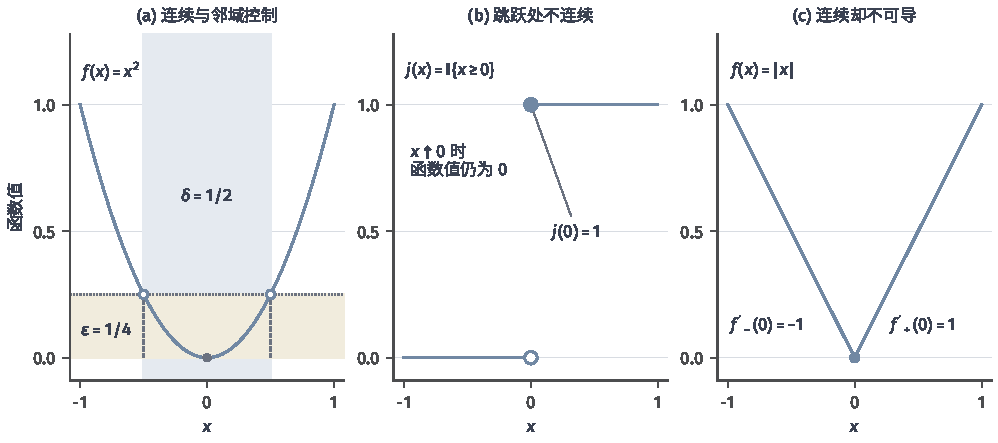
\includegraphics[width=169.0mm]{figures/01-mathematical-preliminaries-upper/02-real-numbers-and-univariate-functions/matplotlib/analysis-continuity-counterexamples/figure.pdf}
 \caption{平方函数、绝对值函数与阶跃函数在原点的差别。平方函数连续且可微；绝对值函数连续，但左右导数不同；阶跃函数的左右极限不同。连续性控制函数值的极限，可微性还要求差商具有同一个有限极限。}
 \label{fig:analysis-continuity-counterexamples}
\end{figure*}

导数的定义可以等价地改写为增量的近似形式。差商趋于$f'(a)$，等价于$[f(a+h)-f(a)-f'(a)h]/h\to0$，即
\begin{equation}
 f(a+h)=f(a)+f'(a)h+o(h),\qquad h\to0.
 \label{eq:analysis-scalar-first-order}
\end{equation}
反过来，若存在实数$A$使$f(a+h)=f(a)+Ah+o(h)$，两边减去$f(a)$、除以$h$再令$h\to0$，可知$f$可导且$A=f'(a)$。
满足这一分解的函数称为在$a$处\term{可微}（differentiable）；对一元函数，可导与可微是同一回事。
这一形式把增量分成两部分：$f'(a)h$是输入增量乘以一个固定系数，称为一次近似；余项相对于$h$可以忽略。
一元情形下，“乘以固定系数”就是最简单的线性关系；多个输入时，这个系数要换成线性映射，留到线性代数部分统一处理。

增量、微分与导数是三个不同的对象。$\Delta f$是实际的函数变化；以$f'(a)$为系数的映射$h\mapsto f'(a)h$称为$f$在$a$处的\term{微分}（differential），常记作$\mathrm df=f'(x)\,\mathrm dx$，其中$\mathrm dx$表示输入增量；
导数$f'(a)$则是这个映射的系数。
\begin{example}[平方函数在$a=3$处的微分]
\label{ex:analysis-square-differential}
设$f(x)=x^2$，$a=3$，则$f'(3)=6$，微分为$6h$。取$h=0.1$，微分给出$0.6$，实际增量为$3.1^2-3^2=0.61$，两者之差$(3+h)^2-9-6h=h^2=0.01$。
\end{example}
一次近似常用来估计误差的传递：测量半径$r$时有误差$\Delta r$，圆面积$\pi r^2$的误差约为$2\pi r\,\Delta r$。
但式~\eqref{eq:analysis-scalar-first-order}中的$o(h)$只说明$h\to0$时余项相对于$h$趋于零，并没有告诉我们在指定的$h=0.1$处余项有多大。
要得到给定步长下可以计算的误差上界，需要后面的中值定理与Taylor公式。

\section{导数的运算规则}
\label{sec:ru-derivative-rules}
\label{sec:analysis-scalar-chain-rules}

直接用定义求导，每个函数都要重新计算差商。若已知几个函数的导数，由它们组合出的函数的导数应能直接算出。
本节在导数已经存在的条件下，分别研究四则运算、复合和取反函数怎样传递到导数，下一节再用这些规则计算基本函数的导数。
以下设$f,g$在所讨论的点$a$的某个开邻域内有定义，并在$a$处可导。

\subsection{导数的四则运算}
\label{sec:ru-derivative-arithmetic}

和的差商等于两个差商之和，常数倍的差商等于差商的同一常数倍，令$h\to0$即得$(f\pm g)'(a)=f'(a)\pm g'(a)$与$(cf)'(a)=cf'(a)$。
乘积的增量可以拆成三部分。记$\Delta f=f(a+h)-f(a)$、$\Delta g=g(a+h)-g(a)$，则
\[
 f(a+h)g(a+h)-f(a)g(a)=g(a)\,\Delta f+f(a)\,\Delta g+\Delta f\,\Delta g.
\]
由一次展开，前两项之和为$[f'(a)g(a)+f(a)g'(a)]h+o(h)$；两个增量都至多与$|h|$同阶，乘积$\Delta f\,\Delta g$与$h^2$同阶，所以也是$o(h)$。读出一次项的系数，得到乘积法则
\begin{equation}
 (fg)'(a)=f'(a)g(a)+f(a)g'(a).
 \label{eq:analysis-scalar-sum-product-rules}
\end{equation}
增量的乘积之所以可以并入余项，是因为两个小量相乘比每个小量都小得多；这一步使乘积的导数只剩两项。

商需要分母非零。设$g(a)\neq0$，可导蕴含连续，所以$g$在$a$附近不为零。先求倒数的导数：
\[
 \frac1h\Bigl(\frac1{g(a+h)}-\frac1{g(a)}\Bigr)=-\frac{g(a+h)-g(a)}h\cdot\frac1{g(a+h)g(a)}\to-\frac{g'(a)}{g(a)^2},
\]
再把$f/g$写成$f\cdot(1/g)$用乘积法则，得到
\[
 \Bigl(\frac fg\Bigr)'(a)=\frac{f'(a)g(a)-f(a)g'(a)}{g(a)^2}.
\]

\subsection{复合函数的求导法则}
\label{sec:ru-chain-rule}

复合函数的输入变化先经过内层、再传入外层，总的一次变化由两层的变化率相乘得到。
\begin{theorem}[链式法则]
\label{thm:ru-chain-rule}
若$f$在$a$处可导，$g$在$f(a)$处可导，且$g\circ f$在$a$的某个邻域内有定义，则
\begin{equation}
 (g\circ f)'(a)=g'(f(a))\,f'(a).
 \label{eq:analysis-scalar-chain-rule}
\end{equation}
\end{theorem}
\begin{proof}
记$b=f(a)$、$k(h)=f(a+h)-f(a)$。由$f$的一次展开，$k(h)=f'(a)h+o(h)$，所以$k(h)\to0$，并且充分小的$h$满足$|k(h)|\leq(|f'(a)|+1)|h|$。
把$g$在$b$处的一次展开写成$g(b+k)=g(b)+g'(b)k+|k|\,\varepsilon(k)$，其中$k\neq0$时$\varepsilon(k)=[g(b+k)-g(b)-g'(b)k]/|k|\to0$，并规定$\varepsilon(0)=0$。代入$k=k(h)$，
\[
 g(f(a+h))-g(f(a))=g'(b)f'(a)h+g'(b)\,o(h)+|k(h)|\,\varepsilon(k(h)).
\]
最后一项的绝对值不超过$(|f'(a)|+1)|h|\,|\varepsilon(k(h))|$，也是$o(h)$。所以一次项系数为$g'(b)f'(a)$。
\end{proof}
证明中规定$\varepsilon(0)=0$，是为了处理内层增量$k(h)$可能为零的情形；若照搬记号$\frac{\mathrm dg}{\mathrm dx}=\frac{\mathrm dg}{\mathrm dy}\cdot\frac{\mathrm dy}{\mathrm dx}$“约去$\mathrm dy$”，就会在$k(h)=0$时除以零。
记号可以帮助记忆，但不能代替证明。用一个能直接展开的例子核对：$(1+x^2)^3$以$y=1+x^2$为中间变量，链式法则给出$3y^2\cdot2x=6x(1+x^2)^2$；
直接展开$(1+x^2)^3=1+3x^2+3x^4+x^6$再求导，得$6x+12x^3+6x^5$，二者相同。

\subsection{反函数的求导法则}
\label{sec:ru-inverse-derivative}

上一章已经证明，区间上连续且严格单调的函数有连续的反函数（定理~\ref{thm:ru-inverse-continuity}）。现在判断反函数何时可导。
设$f$在区间$I$上连续、严格单调，$g=f^{-1}$。设$a$是$I$的内点，$f$在$a$处可导且$f'(a)\neq0$，记$b=f(a)$，$b$是区间$f(I)$的内点。
对充分小的$k\neq0$，令$h=g(b+k)-a$。$g$是单射，所以$h\neq0$；$g$连续，所以$k\to0$时$h\to0$。由$f(a+h)=b+k$，
\[
 \frac{g(b+k)-g(b)}k=\frac h{f(a+h)-f(a)}\to\frac1{f'(a)}.
\]
因此$g$在$b$处可导，且$g'(b)=1/f'(a)$，即$(f^{-1})'(b)=1/f'(f^{-1}(b))$。

对$f(g(y))=y$用链式法则也能得到同一公式，但那要求事先知道$g$可导，所以上面先用差商证明可导性；证明中$h\to0$这一步依赖反函数的连续性。
条件$f'(a)\neq0$不能省略：$x^3$在$0$处导数为零，反函数$\sqrt[3]y$在$0$处的差商为$1/\sqrt[3]{k^2}$，$k\to0$时无界，反函数不可导，图像在原点有一条竖直的切线。
在区间端点只能取单侧差商，结论相应地改为单侧导数。下一节用这一规则求对数与反三角函数的导数。

\section{基本函数的导数}
\label{sec:ru-elementary-derivatives}
\label{sec:analysis-elementary-derivatives}

有了求导规则，复杂函数的求导就归结为少数基本函数。本节先由有限运算和上一章的基本极限得到幂函数、指数和三角函数的导数，
再借反函数与复合的规则得到其余基本函数的导数，并逐项注明成立范围。

常数函数的差商恒为零，恒等函数的差商恒为$1$。对正整数$m$，把$x^m$看成$m$个恒等函数之积，反复使用乘积法则，每一项只对一个因子求导，共$m$项，得$(x^m)'=mx^{m-1}$。
对负整数$m=-n$，在$x\neq0$处由商法则得$(x^{-n})'=-nx^{n-1}/x^{2n}=mx^{m-1}$，形式相同。于是多项式可以逐项求导，例如$(x^3-3x)'=3x^2-3$。

指数函数满足$e^{x+h}=e^xe^h$，由第~\ref{sec:ru-elementary-limits}节的基本极限$(e^h-1)/h\to1$，
\[
 \frac{e^{x+h}-e^x}h=e^x\,\frac{e^h-1}h\to e^x,\qquad\text{即}\ (e^x)'=e^x.
\]
正弦和余弦由加法公式把差商写成两个基本极限的组合：
\[
 \frac{\sin(x+h)-\sin x}h=\sin x\,\frac{\cos h-1}h+\cos x\,\frac{\sin h}h\to\cos x,
\]
同理$(\cos x)'=-\sin x$。这两个推导只用到加法公式和基本极限，不依赖尚未证明的逐项求导；第~\ref{sec:ru-termwise-differentiation}节对指数级数逐项求导会得到同样的结果，可作核对。
由商法则，$(\tan x)'=(\cos^2x+\sin^2x)/\cos^2x=1/\cos^2x=1+\tan^2x$，在$\cos x\neq0$处成立。

其余基本函数是这些函数的反函数或复合。自然对数是指数函数的反函数，指数的导数处处非零，由反函数求导，$(\log x)'=1/e^{\log x}=1/x$（$x>0$）。
反正弦是正弦在$[-\pi/2,\pi/2]$上的反函数。在$(-\pi/2,\pi/2)$内$(\sin)'=\cos>0$，所以对$y\in(-1,1)$，
\[
 (\arcsin y)'=\frac1{\cos(\arcsin y)}=\frac1{\sqrt{1-y^2}},
\]
其中$\cos(\arcsin y)\geq0$保证开方取正号。在$y=\pm1$处，对应的$\cos=0$，反正弦不可导，图像有竖直的切线。
同理$(\arccos y)'=-1/\sqrt{1-y^2}$（$-1<y<1$），而$(\arctan y)'=1/(1+\tan^2(\arctan y))=1/(1+y^2)$对所有实数$y$成立。

一般底数与实数次幂由自然指数和对数定义：$a^x=e^{x\log a}$（$a>0$），$x^\alpha=e^{\alpha\log x}$（$x>0$）。由链式法则，
\[
 (a^x)'=a^x\log a,\qquad (x^\alpha)'=e^{\alpha\log x}\cdot\frac\alpha x=\alpha x^{\alpha-1},\qquad (\log_ax)'=\frac1{x\log a}.
\]
$x^\alpha$的公式只在$x>0$上使用，因为一般实数次幂只对正数定义；$\alpha$为整数时它与前面的结果一致，并且后者在负数处也成立。
表~\ref{tab:analysis-elementary-derivatives}汇总这些公式。把它们与四则运算、链式法则和反函数求导结合，就能求出基本函数经有限次运算与复合得到的函数的导数。

\begin{table}[htbp]
 \centering\small
 \begin{tabular}{@{}lll@{}}
 \toprule
 函数 & 导数 & 成立范围\\
 \midrule
 $x^m$（$m\in\mathbb Z$） & $mx^{m-1}$ & $m\geq0$时$x\in\mathbb R$；$m<0$时$x\neq0$\\
 $x^\alpha$（$\alpha\in\mathbb R$） & $\alpha x^{\alpha-1}$ & $x>0$\\
 $e^x$ & $e^x$ & $x\in\mathbb R$\\
 $a^x$（$a>0$） & $a^x\log a$ & $x\in\mathbb R$\\
 $\log x$ & $1/x$ & $x>0$\\
 $\log_ax$（$a>0$，$a\neq1$） & $1/(x\log a)$ & $x>0$\\
 $\sin x$ & $\cos x$ & $x\in\mathbb R$\\
 $\cos x$ & $-\sin x$ & $x\in\mathbb R$\\
 $\tan x$ & $1/\cos^2x$ & $x\neq\pi/2+k\pi$\\
 $\arcsin x$ & $1/\sqrt{1-x^2}$ & $-1<x<1$\\
 $\arccos x$ & $-1/\sqrt{1-x^2}$ & $-1<x<1$\\
 $\arctan x$ & $1/(1+x^2)$ & $x\in\mathbb R$\\
 \bottomrule
 \end{tabular}
 \caption{基本函数的导数及成立范围。三角函数采用弧度制，$\log$为自然对数。}
 \label{tab:analysis-elementary-derivatives}
\end{table}

\section{高阶导数}
\label{sec:ru-higher-derivatives}

导函数本身也可以求导。若$f'$在某点可导，它在该点的导数称为$f$的二阶导数，记作$f''$；依次定义$f^{(n)}=(f^{(n-1)})'$，约定$f^{(0)}=f$。
例如$f(x)=x^3-3x$时，$f'(x)=3x^2-3$，$f''(x)=6x$，$f'''\equiv6$，四阶及以上导数为零；$e^x$的各阶导数都是$e^x$；$\sin x$的导数按$\cos x,-\sin x,-\cos x,\sin x$四步一循环。

高阶导数存在与高阶导数连续是两个不同的条件。若$f$在开区间$I$上直到$n$阶导数都存在且连续，称$f$为$n$阶\term{连续可微}（continuously differentiable）函数，记作$f\in C^n(I)$；各阶导数都存在时记作$f\in C^\infty(I)$。
多项式、指数和三角函数都属于$C^\infty$。下面的例子说明处处可导的函数，导函数可以不连续。
\begin{example}[处处可导而导函数不连续]
\label{ex:analysis-derivative-not-continuous}
令$f(0)=0$，$x\neq0$时$f(x)=x^2\sin(1/x)$。在原点，差商$h\sin(1/h)$被$\pm|h|$夹住，趋于$0$，所以$f'(0)=0$。在$x\neq0$处，由乘积法则和链式法则，
\[
 f'(x)=2x\sin\frac1x-\cos\frac1x.
\]
取$x_n=1/(2n\pi)\to0$，则$f'(x_n)=-1$，不趋于$f'(0)=0$。所以$f$处处可导，但不属于$C^1(\mathbb R)$，更没有二阶导数$f''(0)$。
\end{example}
导数在原点附近的振荡来自$-\cos(1/x)$一项。可见“$n$阶可导”与“属于$C^n$”需要分别验证；后面的Taylor公式会明确写出用到的是哪一种条件。

乘积的高阶导数有类似二项式定理的公式。对$n$归纳，并用组合数的递推$\binom nk+\binom n{k-1}=\binom{n+1}k$合并同类项，得到Leibniz公式
\[
 (fg)^{(n)}=\sum_{k=0}^n\binom nkf^{(k)}g^{(n-k)},
\]
其中$f,g$在所讨论的点$n$阶可导。例如$(x^2e^x)^{(n)}$中，$x^2$三阶以上的导数为零，只剩三项：
\[
 (x^2e^x)^{(n)}=x^2e^x+n\cdot2x\,e^x+\binom n2\cdot2\,e^x=e^x\bigl(x^2+2nx+n(n-1)\bigr).
\]

复合函数逐层求导时，每次求导都要再用一次链式法则或乘积法则。以第~\ref{sec:ru-function-arithmetic}节的复合函数$g(x)=\sqrt{1-x^2}$为例，在$(-1,1)$上，
\[
 g'(x)=\frac{-2x}{2\sqrt{1-x^2}}=-\frac x{\sqrt{1-x^2}},\qquad
 g''(x)=-\frac{\sqrt{1-x^2}+x^2/\sqrt{1-x^2}}{1-x^2}=-\frac1{(1-x^2)^{3/2}}.
\]
对参数函数族，求导的变量要说清楚：$f_{a,b}(x)=ax+b$关于输入$x$的导数是$a$，二阶导数为$0$；若把$x$固定、改变参数$a$，函数值的变化率则是$x$。
这些逐层计算得到的各阶导数，正是下面Taylor展开所需的系数。

\section{闭区间上可微函数的性质}
\label{sec:ru-interval-differentiable}

导数记录一点处的变化率。本节把它与区间上的极值、净变化、增减方向、弯曲方向以及变化幅度联系起来。
主要对象是在闭区间上连续、在区间内部可微的函数；局部极值与驻点先在内点讨论，各结论分别写明是否需要端点连续、单侧导数或导数的界。

\subsection{局部极值与驻点}
\label{sec:ru-local-extrema}

导数只反映一点附近的变化，与它对应的是只比较邻近函数值的极值。设$c$属于$f$的定义域，若存在$r>0$，使定义域中满足$|x-c|<r$的$x$都有$f(x)\geq f(c)$，
则称$c$为$f$的局部极小点；若其中$x\neq c$的点都满足$f(x)>f(c)$，称为严格局部极小点。不等号反向，得到局部极大点。
局部极值只与附近比较，整个定义域上的最值则与全部输入比较；最小点一定是局部极小点，反之不然。
\begin{theorem}[Fermat定理]
\label{thm:analysis-fermat}
设$c$是区间$I$的内点，$f:I\to\mathbb R$在$c$处可导。若$c$为$f$的局部极小点或局部极大点，则
\begin{equation}
 f'(c)=0.
 \label{eq:analysis-scalar-first-order-necessary}
\end{equation}
\end{theorem}
\begin{proof}
设$c$为局部极小点。充分小的$h\neq0$满足$f(c+h)-f(c)\geq0$，所以$h>0$时差商非负，$h<0$时差商非正。两侧差商趋于同一个导数，于是$f'(c)\geq0$且$f'(c)\leq0$。局部极大点对$-f$论证。
\end{proof}
导数为零的点称为\term{驻点}（stationary point）。Fermat定理说明，内点处可导的局部极值点必为驻点。证明用到了从两侧取差商，所以结论只适用于内点。

在闭区间上找最值时，极值定理保证最值存在，Fermat定理则缩小了候选范围：最值点只可能是端点、内部驻点，或者内部不可导的点。
例如$f(x)=x^3-3x$在$[-2,3]$上，$f'(x)=3(x-1)(x+1)$，驻点为$\pm1$。比较$f(-2)=-2$、$f(-1)=2$、$f(1)=-2$、$f(3)=18$，最大值$18$在端点$3$取得，最小值$-2$在$-2$与$1$两处取得。
导数为零只是内点极值的必要条件。$x^3$在$0$处导数为零，但$x<0$时$x^3<0$、$x>0$时$x^3>0$，$0$不是极值点。
不可导的点也要单独检查：$|x|$在$0$处取最小值，那里没有导数；端点$0$是$x$在$[0,1]$上的最小点，右导数却是$1$。

\subsection{中值定理}
\label{sec:ru-mean-value-theorems}

若函数在区间两端取同一值，整段的净变化为零；在连续、可导的条件下，区间内部必有一点的瞬时变化率也为零。
\begin{theorem}[Rolle定理]
\label{thm:analysis-rolle}
设$a<b$，$f$在$[a,b]$上连续、在$(a,b)$内可导，且$f(a)=f(b)$，则存在$c\in(a,b)$使$f'(c)=0$。
\end{theorem}
\begin{proof}
若$f$为常数，任取$c$即可。否则$f$在某个内点的值不同于$f(a)$。由极值定理，$f$在$[a,b]$上达到最大值和最小值，其中至少有一个与端点值不同，因而在某个内点$c$取得。
$c$是局部极值点，$f$在那里可导，由Fermat定理$f'(c)=0$。
\end{proof}
两端取值不同时，先减去连接两端点的直线，使剩余部分在两端相等，再用Rolle定理。
\begin{theorem}[Lagrange中值定理]
\label{thm:analysis-lagrange-mean-value}
设$a<b$，$f$在$[a,b]$上连续、在$(a,b)$内可导，则存在$c\in(a,b)$使
\begin{equation}
 f(b)-f(a)=f'(c)(b-a).
 \label{eq:analysis-mean-value-theorem}
\end{equation}
\end{theorem}
\begin{proof}
令$H(x)=f(x)-f(a)-\frac{f(b)-f(a)}{b-a}(x-a)$，则$H$满足Rolle定理的条件，且$H(a)=H(b)=0$。由$H'(c)=0$整理即得。
\end{proof}
这就是\term{中值定理}（mean value theorem）的含义：区间上的平均变化率等于某个内点处的瞬时变化率。定理只要求内点可导，不要求导函数连续，也不要求端点的单侧导数存在。
图~\ref{fig:analysis-process-mean-value-parallel}以$f(x)=x^2$、区间$[0,1]$为例：端点割线的斜率为$1$，$c=1/2$处的切线与之平行。

\begin{figure}[!htbp]
 \centering
 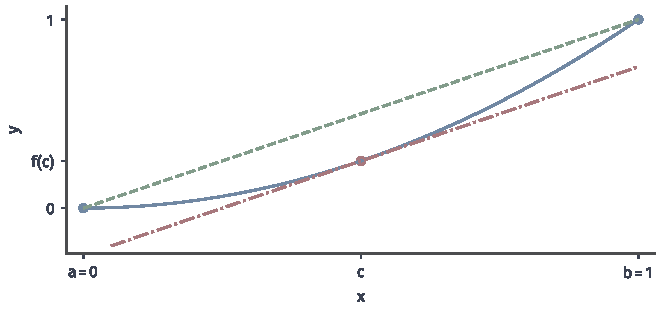
\includegraphics[width=112.0mm]{figures/01-mathematical-preliminaries-upper/00-shared/matplotlib/chapter3-concept-processes/mean-value-parallel.pdf}
 \caption{$f(x)=x^2$在$[0,1]$上，绿虚线为端点割线，红点划线为$c=1/2$处的切线。两线平行，因为$f'(c)=1=[f(1)-f(0)]/(1-0)$。两线高度不同：相等的是斜率，两条直线并不重合。}
 \label{fig:analysis-process-mean-value-parallel}
\end{figure}

比较两个函数在同一区间上的变化时，可以把两者的端点增量放进同一个辅助函数。结论先写成交叉相乘的形式，不需要假设任何分母非零。
\begin{theorem}[Cauchy中值定理]
\label{thm:analysis-cauchy-mean-value}
设$a<b$，$f,g$都在$[a,b]$上连续、在$(a,b)$内可导，则存在$c\in(a,b)$使
\[
 \bigl(f(b)-f(a)\bigr)g'(c)=\bigl(g(b)-g(a)\bigr)f'(c).
\]
若还有$g'(x)\neq0$对每个$x\in(a,b)$成立，则$g(b)\neq g(a)$，并且
\[
 \frac{f(b)-f(a)}{g(b)-g(a)}=\frac{f'(c)}{g'(c)}.
\]
\end{theorem}
\begin{proof}
令$H(x)=(f(b)-f(a))(g(x)-g(a))-(g(b)-g(a))(f(x)-f(a))$，则$H(a)=H(b)=0$，由Rolle定理得$H'(c)=0$，展开即为交叉相乘形式。
若$g'$在内部处处非零，$g(b)=g(a)$会使Rolle定理给出某个内点处$g'=0$，所以$g(b)\neq g(a)$；两边同除以非零的$(g(b)-g(a))g'(c)$即得比值形式。
\end{proof}
取$g(x)=x$即回到Lagrange中值定理。写成比值时要先检查分母：比值形式依赖$g'$在内部处处非零，第~\ref{sec:ru-lhopital}节的L'Hôpital法则正是用这一形式证明的。

\subsection{单调性与凹凸性}
\label{sec:ru-monotonicity-convexity}
\label{sec:analysis-monotonicity}

中值定理把任意两点之间的增量写成某个内点处的导数乘以输入增量，所以导数的符号可以控制整段的增减。
\begin{theorem}[导数符号与单调性]
\label{thm:analysis-derivative-monotonicity}
设$f$在区间$[a,b]$上连续、在$(a,b)$内可导。若在$(a,b)$内$f'\geq0$，则$f$在$[a,b]$上单调不减；若$f'>0$，则严格递增。$f'\leq0$与$f'<0$相应地给出单调不增与严格递减；若$f'\equiv0$，则$f$为常数。
\end{theorem}
\begin{proof}
任取$a\leq x<y\leq b$，在$[x,y]$上用Lagrange中值定理，$f(y)-f(x)=f'(\xi)(y-x)$，右侧的符号由$f'(\xi)$决定。
\end{proof}
关键是两点之间的整段都属于定义域。在$(0,1)\cup(2,3)$上左段取$0$、右段取$1$的函数导数处处为零，却不是常数，中值定理不能跨过定义域的缺口。
导数处处为正是严格递增的充分条件而非必要条件：$x^3$在$\mathbb R$上严格递增，但在$0$处导数为零。

同样的论证可以判断驻点是否为极值：若$f'$在$c$左侧为负、右侧为正，则$f$在$c$左侧严格递减、右侧严格递增，$c$是严格局部极小点；左正右负则为严格局部极大点。
例如$x^3-3x$的导数$3(x-1)(x+1)$在$1$的左侧为负、右侧为正，$1$是严格局部极小点；在$-1$两侧由正变负，$-1$是严格局部极大点。
若导数在驻点两侧同号，如$x^3$在$0$两侧都有$3x^2>0$，函数沿同一方向变化，驻点就不是极值点。

函数自身的单调性由$f'$的符号决定；$f'$本身的单调性则描述图像的弯曲方向。在区间上任取两点，连接图像上对应两点的线段称为弦。
\begin{definition}[凸函数]
\label{def:ru-convex-function}
设$f$定义在区间$I$上。若对任意$x,y\in I$与$\lambda\in[0,1]$，都有
\[
 f\bigl(\lambda x+(1-\lambda)y\bigr)\leq\lambda f(x)+(1-\lambda)f(y),
\]
即两点之间的图像不高于弦，就称$f$为\term{凸函数}（convex function）；$x\neq y$、$0<\lambda<1$时不等式总是严格成立，称为严格凸函数。若$-f$是凸函数，称$f$为凹函数。
\end{definition}
例如$x^2$是凸函数：$\lambda x^2+(1-\lambda)y^2-(\lambda x+(1-\lambda)y)^2=\lambda(1-\lambda)(x-y)^2\geq0$，并且$x\neq y$时严格大于零。

\begin{theorem}[可微凸函数的刻画]
\label{thm:ru-convexity-derivative}
设$f$在开区间$I$上可微，则下面三条等价：
(1) $f$是凸函数；(2) $f'$在$I$上单调不减；(3) 对任意$x,y\in I$，$f(y)\geq f(x)+f'(x)(y-x)$，即图像总在每条切线的上方。
\end{theorem}
\begin{proof}
(1)$\Rightarrow$(2)：设$x<z<y$，把$z$写成$\lambda x+(1-\lambda)y$，其中$\lambda=(y-z)/(y-x)$，凸性不等式整理后就是三条弦的斜率关系
\[
 \frac{f(z)-f(x)}{z-x}\leq\frac{f(y)-f(x)}{y-x}\leq\frac{f(y)-f(z)}{y-z}.
\]
令$z\to x^+$，左边趋于$f'(x)$；令$z\to y^-$，右边趋于$f'(y)$。所以$f'(x)\leq\frac{f(y)-f(x)}{y-x}\leq f'(y)$。

(2)$\Rightarrow$(3)：由中值定理，$f(y)-f(x)=f'(\xi)(y-x)$，$\xi$在$x,y$之间。$y>x$时$\xi>x$，$f'(\xi)\geq f'(x)$，所以$f(y)-f(x)\geq f'(x)(y-x)$；$y<x$时$f'(\xi)\leq f'(x)$而$y-x<0$，结论相同。

(3)$\Rightarrow$(1)：令$z=\lambda x+(1-\lambda)y$，在$z$处的切线不等式给出$f(x)\geq f(z)+f'(z)(x-z)$与$f(y)\geq f(z)+f'(z)(y-z)$。
两式分别乘以$\lambda$与$1-\lambda$再相加，右侧的一次项因$\lambda(x-z)+(1-\lambda)(y-z)=0$而消去，得到$\lambda f(x)+(1-\lambda)f(y)\geq f(z)$。
\end{proof}
图~\ref{fig:ru-convex-chord-tangent}画出了凸函数与它的一条弦和一条切线：弦在图像上方，切线在图像下方。
凸性要求的是$f'$单调不减，而不是$f$单调：$x^2$在$\mathbb R$上不单调，却是凸函数。

\begin{figure}[!htbp]
 \centering
 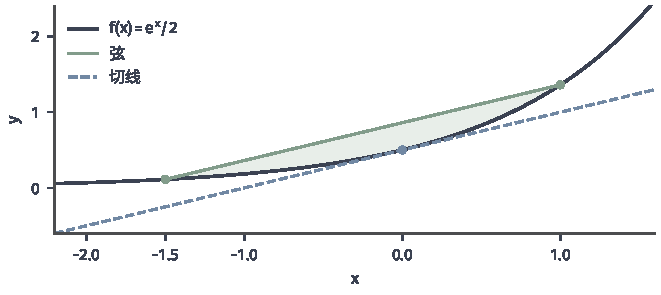
\includegraphics[width=112mm]{figures/01-mathematical-preliminaries-upper/02-real-numbers-and-univariate-functions/matplotlib/convex-chord-tangent/figure.pdf}
 \caption{凸函数$f(x)=e^{x}/2$的弦与切线。绿线连接$x=-1.5$与$x=1$处的两点，两点之间的图像在弦的下方；蓝线是$x=0$处的切线$y=\tfrac12+\tfrac12x$，整条图像在它的上方。图为解析示例。}
 \label{fig:ru-convex-chord-tangent}
\end{figure}

在二阶可微的条件下，凸性可以由二阶导数判断。若$f$在开区间$I$上二阶可导且$f''\geq0$，由定理~\ref{thm:analysis-derivative-monotonicity}，$f'$单调不减，所以$f$是凸函数；
若$f''>0$，则$f'$严格递增，把上面证明中的不等号改为严格，可知$f$严格凸。反方向只对非严格情形成立：凸函数满足$f''\geq0$，因为单调不减的$f'$的导数非负。
严格凸却不要求$f''$处处严格为正。$x^4$的导数$4x^3$在$\mathbb R$上严格递增，所以$x^4$严格凸，但$f''(0)=0$。“二阶导数处处为正”是严格凸的充分条件，不是必要条件。
二阶导数也能判断驻点：若$f'(c)=0$且$f''(c)>0$，则$f'(c+h)/h\to f''(c)>0$，充分小的$h$使$f'(c+h)$与$h$同号，由一阶判别，$c$是严格局部极小点；$f''(c)<0$时是严格局部极大点。
$f''(c)=0$时没有结论：$x^4$、$-x^4$与$x^3$在原点的一、二阶导数都为零，原点分别是极小点、极大点和非极值点。

最后，若导数有统一的界，中值定理把它转化为变化幅度的界。
\begin{theorem}[有界导数与Lipschitz条件]
\label{thm:analysis-bounded-derivative-lipschitz}
设$f$在$[a,b]$上连续、在$(a,b)$内可导，且$|f'(x)|\leq L$对所有$x\in(a,b)$成立，则对任意$x,y\in[a,b]$，$|f(y)-f(x)|\leq L|y-x|$。
\end{theorem}
\begin{proof}
$x\neq y$时，由中值定理$|f(y)-f(x)|=|f'(\xi)|\,|y-x|\leq L|y-x|$。
\end{proof}
例如$\sin$的导数绝对值不超过$1$，所以$|\sin x-\sin y|\leq|x-y|$对所有实数成立。闭区间上的$C^1$函数，导数连续因而有界，于是都是Lipschitz函数。
这说明局部导数信息在具备区间条件时可以给出整体控制。反过来，Lipschitz连续不保证可导：$|x|$在$[-1,1]$上的Lipschitz常数为$1$，在$0$处却不可导。
一元凸性的这些结论将在最优化部分推广到多元函数，并用于判断最优点（第~\ref{chap:optimization}章）。

\section{Taylor公式与局部近似}
\label{sec:ru-taylor}
\label{sec:analysis-taylor-approximation}

一次近似$f(a)+f'(a)h$只用到函数值和斜率，误差是$o(h)$。要提高精度，可以让近似多项式在$a$处与$f$有更多阶相同的导数。
本节先说明这样的多项式怎样确定、误差怎样控制，再把它用于指数函数和三角函数，得到它们的级数展开与Euler公式，最后用同样的工具分析差分近似的误差。

\subsection{Taylor多项式及余项}
\label{sec:ru-taylor-remainders}

设$p(x)=\sum_{k=0}^nc_k(x-a)^k$。逐次求导并代入$x=a$，除了第$k$项外的各项都变为零，得到$p^{(k)}(a)=k!\,c_k$。
所以，要让$p$在$a$处与$f$的前$n$阶导数都相同，系数只能取$c_k=f^{(k)}(a)/k!$。称
\[
 T_n(a+h)=\sum_{k=0}^n\frac{f^{(k)}(a)}{k!}h^k
\]
为$f$在$a$处的$n$阶\term{Taylor多项式}（Taylor polynomial），阶乘来自对$h^k$求$k$次导数。$n=1$时它就是一次近似。
截去的部分$R_n(h)=f(a+h)-T_n(a+h)$称为余项，把函数写成Taylor多项式加余项的等式称为\term{Taylor公式}（Taylor formula）。首先关心的是$h\to0$时余项的阶。
\begin{theorem}[带Peano余项的Taylor公式]
\label{thm:ru-taylor-peano}
设$n\geq1$，$f$在$a$的某个邻域内$n-1$阶可导，且$f^{(n)}(a)$存在，则$h\to0$时
\[
 f(a+h)=\sum_{k=0}^n\frac{f^{(k)}(a)}{k!}h^k+o(h^n).
\]
\end{theorem}
\begin{proof}
对$n$归纳。$n=1$就是可微的定义~\eqref{eq:analysis-scalar-first-order}。设结论对$n-1$成立。$R_n$在$h=0$处为零，它关于$h$的导数$R_n'(h)=f'(a+h)-\sum_{k=1}^n\frac{f^{(k)}(a)}{(k-1)!}h^{k-1}$
恰是$f'$在$a$处的$n-1$阶余项，由归纳假设为$o(h^{n-1})$。由中值定理，$R_n(h)=R_n(h)-R_n(0)=R_n'(\xi)h$，$\xi$在$0$与$h$之间，于是$|R_n(h)|\leq\sup_{|t|\leq|h|}|R_n'(t)|\cdot|h|=o(h^n)$。
\end{proof}
Peano余项只说明误差的阶，不给出指定$h$处的误差大小。若函数在整段上有更高阶的导数，可以把余项写成某个中间点处的导数。
\begin{theorem}[带Lagrange余项的Taylor公式]
\label{thm:analysis-taylor-lagrange}
设$n\geq0$，$h\neq0$，$f$在包含$a$与$a+h$之间闭线段的某个开区间上$n+1$阶可导，则存在严格位于$a$与$a+h$之间的$\xi$，使
\begin{equation}
 f(a+h)=\sum_{k=0}^n\frac{f^{(k)}(a)}{k!}h^k+\frac{f^{(n+1)}(\xi)}{(n+1)!}h^{n+1}.
 \label{eq:analysis-taylor-arbitrary-order}
\end{equation}
若该线段上$|f^{(n+1)}|\leq M$，则$|R_n(h)|\leq M|h|^{n+1}/(n+1)!$。
\end{theorem}
\begin{proof}
记$T(t)=\sum_{k=0}^nf^{(k)}(a)(t-a)^k/k!$，$R=f(a+h)-T(a+h)$，令$H(t)=f(t)-T(t)-R\,(t-a)^{n+1}/h^{n+1}$。
则$H(a+h)=0$，且$H(a)=H'(a)=\cdots=H^{(n)}(a)=0$。先在$a$与$a+h$之间对$H$用Rolle定理得$\xi_1$使$H'(\xi_1)=0$；再在$a$与$\xi_1$之间对$H'$用Rolle定理得$\xi_2$，如此继续。
共用$n+1$次后得到严格位于$a$与$a+h$之间的$\xi$，使$H^{(n+1)}(\xi)=0$。由$T^{(n+1)}=0$，这就是$f^{(n+1)}(\xi)-(n+1)!\,R/h^{n+1}=0$。
\end{proof}
$n=0$时公式就是Lagrange中值定理。误差界说明近似的精度同时取决于阶数、步长和高阶导数的界，三者都可以具体计算。
例如$f(x)=x^3-3x$在$a=1/2$处的二阶Taylor多项式为$T_2=-\tfrac{11}8-\tfrac94h+\tfrac32h^2$，由$f'''\equiv6$，余项恰为$h^3$；取$h=0.1$，$T_2$与真值$-1.584$相差$0.001$。
余项的第三种写法是积分形式，它不含未知的中间点，需要积分，留到第~\ref{sec:ru-integration-by-parts}节推导。

有限阶展开、Taylor级数与“函数等于自身的Taylor级数”是三件不同的事。若$f$无穷次可微，可以写出无穷级数$\sum_kf^{(k)}(a)(x-a)^k/k!$，称为$f$在$a$处的Taylor级数；
但这个级数未必收敛到$f$。下面的例子中，Taylor级数在整条实轴上收敛，却只在一点等于原函数。
\begin{example}[光滑但不等于自身Taylor级数的函数]
\label{ex:ru-smooth-not-analytic}
令$f(0)=0$，$x\neq0$时$f(x)=e^{-1/x^2}$。对$x\neq0$归纳可知$f^{(k)}(x)=P_k(1/x)e^{-1/x^2}$，其中$P_k$是多项式。
由$e^u\geq u^m/m!$（$u>0$）取$u=1/x^2$，得$|x|^{-j}e^{-1/x^2}\leq m!\,|x|^{2m-j}$，取$2m>j$即知它在$x\to0$时趋于零。
再在原点用差商逐阶验证，可得$f^{(k)}(0)=0$对每个$k$成立。于是$f$的Taylor级数恒为零，而$x\neq0$时$f(x)>0$。
\end{example}
所以无穷次可微还不足以保证函数能由Taylor级数表示。对具体函数，必须另外证明余项趋于零；下面对指数和三角函数完成这一步。

\subsection{指数函数的展开}
\label{sec:ru-exp-expansion}

由$(e^x)'=e^x$，指数函数在$0$处的各阶导数都是$1$，Taylor系数为$1/k!$。由Lagrange余项，对固定的$x$，
\[
 \Bigl|e^x-\sum_{k=0}^n\frac{x^k}{k!}\Bigr|=\frac{e^\xi|x|^{n+1}}{(n+1)!}\leq\frac{e^{|x|}|x|^{n+1}}{(n+1)!},
\]
$\xi$在$0$与$x$之间。右侧是收敛级数$\sum|x|^k/k!$的项，趋于零，所以余项趋于零，$e^x=\sum_{k\geq0}x^k/k!$。
这与第~\ref{sec:ru-elementary-limits}节用级数定义的指数一致。那里级数是定义，这里则是从导数出发，用余项估计证明函数等于级数，两条路线得到同一个对象。

余项估计还说明了截断要取多少项。在区间$[-A,A]$上，误差不超过$e^AA^{n+1}/(n+1)!$，这个界对整个区间统一成立。
例如$A=1$、$n=7$时误差不超过$e/8!\approx6.7\times10^{-5}$；区间越大，所需阶数越高。一般底数的指数$a^x=e^{x\log a}$可以把$x\log a$代入上式处理。

\subsection{三角函数的展开与复指数}
\label{sec:ru-trig-expansion-complex-exponential}

正弦和余弦的各阶导数按四步循环，在$0$处的值依次为$\sin$：$0,1,0,-1,\ldots$，$\cos$：$1,0,-1,0,\ldots$。各阶导数的绝对值都不超过$1$，Lagrange余项满足$|R_n(x)|\leq|x|^{n+1}/(n+1)!\to0$，所以
\[
 \sin x=\sum_{k=0}^\infty\frac{(-1)^kx^{2k+1}}{(2k+1)!},\qquad\cos x=\sum_{k=0}^\infty\frac{(-1)^kx^{2k}}{(2k)!},
\]
对所有实数$x$成立。截断误差也可以直接读出：$\sin x\approx x-x^3/6$的四次项为零，用$n=4$的余项得误差不超过$|x|^5/120$；$x=0.5$时约为$2.6\times10^{-4}$。

这两个级数与指数级数只差符号的排列，提示三者有联系。为看清这一点，需要让指数级数接受复数输入。
复数列$z_n\to z$定义为$|z_n-z|\to0$；由$|\operatorname{Re}w|,|\operatorname{Im}w|\leq|w|\leq|\operatorname{Re}w|+|\operatorname{Im}w|$，它等价于实部、虚部分别收敛。
若$\sum|z_k|<\infty$，则实部级数与虚部级数都绝对收敛，因而$\sum z_k$收敛，绝对收敛的结论由此搬到复数。
对每个复数$z$，$\sum|z|^k/k!=e^{|z|}$有限，所以可以定义复指数
\[
 e^z=\sum_{k=0}^\infty\frac{z^k}{k!}.
\]
取纯虚输入$z=i\theta$。由$i^2=-1$，$i^k$按$1,i,-1,-i$循环，部分和$S_{2N+1}$的偶次项全为实数、奇次项全为虚数：
\[
 S_{2N+1}(i\theta)=\sum_{k=0}^N\frac{(-1)^k\theta^{2k}}{(2k)!}+i\sum_{k=0}^N\frac{(-1)^k\theta^{2k+1}}{(2k+1)!}.
\]
令$N\to\infty$，实部与虚部分别趋于刚证明的余弦与正弦展开；整个级数收敛，它的和等于这个子列的极限。于是得到\term{Euler公式}（Euler's formula）
\[
 e^{i\theta}=\cos\theta+i\sin\theta.
\]
这里只把偶次项与奇次项分开读出，没有改变求和次序。

回到复数的三角形式$z=r(\cos\theta+i\sin\theta)$，Euler公式把它写成指数形式$z=re^{i\theta}$：$r$是模，$\theta$是辐角。
第~\ref{sec:ru-complex-geometry}节的“模相乘、辐角相加”变为$r_1e^{i\theta_1}\cdot r_2e^{i\theta_2}=r_1r_2e^{i(\theta_1+\theta_2)}$，整数次幂变为$(re^{i\theta})^n=r^ne^{in\theta}$，三角形式与指数形式由此统一。
特别地，$e^{i\pi}=-1$，$e^{2\pi i}=1$，辐角相差$2\pi$的整数倍正对应$e^{i\theta}$的周期性。本书只使用复数级数，不展开复变函数的微积分。

\subsection{差分近似和步长选择}
\label{sec:ru-finite-differences}

只能计算函数值时，常用差商近似导数。Taylor公式可以说明这种近似的误差有多大。设$f$在$x$附近足够光滑，前向差分的误差由二阶Taylor公式得到：
\[
 \frac{f(x+h)-f(x)}h=f'(x)+\frac{f''(\xi)}2h,
\]
所以$|f''|\leq M_2$时截断误差不超过$M_2h/2$，与$h$同阶。中心差分对称地取两侧，把$f(x\pm h)$各展开到三阶后相减，偶次项抵消：
\[
 \frac{f(x+h)-f(x-h)}{2h}=f'(x)+\frac{f'''(\xi_1)+f'''(\xi_2)}{12}h^2,
\]
$|f'''|\leq M_3$时误差不超过$M_3h^2/6$，与$h^2$同阶，代价是需要三阶导数的界。
用$f(x)=e^x$在$x=0$处核对：取$h=0.1$，前向差分为$(e^{0.1}-1)/0.1\approx1.0517$，误差约$0.052$，接近$h/2=0.05$；中心差分为$(e^{0.1}-e^{-0.1})/0.2\approx1.00167$，误差约$0.00167$，接近$h^2/6\approx0.00167$。

上面的误差分析假定函数值是精确的。实际计算中，函数值本身带有数据误差或舍入误差。设算得的值$\tilde f$满足$|\tilde f-f|\leq\eta$，前向差分的总误差就不超过
\[
 \frac{M_2h}2+\frac{2\eta}h.
\]
第一项是截断误差，随$h$减小而减小；第二项是函数值误差，被除以$h$后放大，随$h$减小而增大。两者之和在$h=2\sqrt{\eta/M_2}$处最小，最小值为$2\sqrt{M_2\eta}$。
以双精度浮点计算为例，$\eta$约为$10^{-16}$乘以函数值的大小，前向差分的合适步长约为$10^{-8}$，而不是越小越好；中心差分的总误差为$M_3h^2/6+\eta/h$，合适步长约为$10^{-5}$\scite{math-nocedal2006numerical}。
图~\ref{fig:ru-finite-difference-error}画出了实际计算的误差：步长大于最优值时，误差沿截断误差的斜率下降；小于最优值后，舍入误差占主导，误差反而上升并剧烈波动。
这里只讨论误差的来源与竞争，系统的数值分析不在本书范围之内。

\begin{figure}[!htbp]
 \centering
 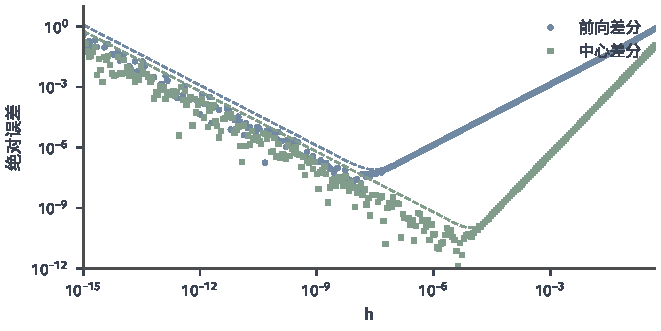
\includegraphics[width=112mm]{figures/01-mathematical-preliminaries-upper/02-real-numbers-and-univariate-functions/matplotlib/finite-difference-error/figure.pdf}
 \caption{用双精度浮点数计算$f(x)=e^x$在$x=1$处导数的差分误差，横轴为步长$h$，两轴均为对数刻度。蓝点为前向差分，绿点为中心差分；虚线是误差模型$eh/2+2\epsilon_{\mathrm{m}}e/h$与$eh^2/6+\epsilon_{\mathrm{m}}e/h$，$\epsilon_{\mathrm{m}}\approx2.2\times10^{-16}$为机器精度。大步长段的斜率分别为$1$与$2$，小步长段的误差随$h$减小而增大。}
 \label{fig:ru-finite-difference-error}
\end{figure}

\section{不定式与L'Hôpital法则}
\label{sec:ru-lhopital}

两个都趋于零的函数相除，比值的极限不能由各自的极限算出，这类形式称为不定式。它问的其实是两个无穷小谁更快趋于零。
函数在趋近点附近可微时，两个函数的增量都可以用导数描述，于是可以借导数比较它们。

\begin{theorem}[L'Hôpital法则]
\label{thm:ru-lhopital}
设$f,g$在$(a,a+r)$内可导，$g'\neq0$，并且$x\to a^+$时$f(x)\to0$、$g(x)\to0$。若$f'(x)/g'(x)\to L$，其中$L$为实数或$\pm\infty$，则$f(x)/g(x)\to L$。左侧与双侧极限有相同的结论。
\end{theorem}
\begin{proof}
补充定义$f(a)=g(a)=0$，则$f,g$在每个$[a,x]$（$x<a+r$）上连续、在内部可导。由Cauchy中值定理的比值形式，存在$\xi_x\in(a,x)$使
\[
 \frac{f(x)}{g(x)}=\frac{f(x)-f(a)}{g(x)-g(a)}=\frac{f'(\xi_x)}{g'(\xi_x)}.
\]
$x\to a^+$时$\xi_x\to a^+$，右侧趋于$L$。比值形式所需的$g(x)\neq g(a)$由$g'\neq0$保证。
\end{proof}
定理中的条件都是充分条件：在趋近点的一侧可导、分母的导数非零、导数比有极限。例如
\[
 \lim_{x\to0}\frac{e^x-1-x}{x^2}=\lim_{x\to0}\frac{e^x-1}{2x}=\frac12,
\]
第二个极限仍是$0/0$型，它由基本极限$(e^x-1)/x\to1$直接得到。法则对$x\to\pm\infty$以及分子分母都趋于无穷的$\infty/\infty$型也成立，证明思路相同\scite{math-lebl-analysis1}。

其他不定式要先转换成$0/0$或$\infty/\infty$，再检查条件。$x\to0^+$时$x\log x$是$0\cdot\infty$型，写成$\log x/(1/x)$后为$\infty/\infty$型，导数比$(1/x)/(-1/x^2)=-x\to0$，所以$x\log x\to0$。
$1^\infty$与$0^0$型先取对数：$(1+1/n)^n=e^{n\log(1+1/n)}$，而$n\log(1+1/n)=\log(1+t)/t$（$t=1/n$）趋于$\log$在$1$处的导数$1$，由指数的连续性，$(1+1/n)^n\to e$。

法则不是万能的，有三点要注意。第一，导数比的极限不存在时，原极限仍可能存在：$x\to+\infty$时$(x+\sin x)/x\to1$，导数比$1+\cos x$却在$0$与$2$之间振荡。
第二，夹逼和等价无穷小比较仍然是独立的工具，很多时候更直接。第三，不能用L'Hôpital法则回头证明$\sin h/h\to1$或$(e^h-1)/h\to1$：
对前者使用法则需要$(\sin)'(0)=1$，而这个导数正是从该极限算出来的，论证会循环。基本极限只能像第~\ref{sec:ru-elementary-limits}节那样用几何或级数直接估计。

\section{函数项级数和幂级数的逐项求导}
\label{sec:ru-termwise-differentiation}

有限和的导数等于各项导数之和。对函数项级数，能否同样逐项求导，就是能否交换“求导”与“取极限”两个操作。
上一章已经看到一致收敛能保持连续性，但下面的例子说明，它不足以保持导数。

令$f_n(x)=\sin(n^2x)/n$。由$|f_n(x)|\leq1/n$，$f_n$在$\mathbb R$上一致收敛到$0$，极限函数的导数为$0$；但$f_n'(x)=n\cos(n^2x)$，在$x=0$处等于$n\to\infty$，并不收敛。
函数值的振幅虽小，振荡的频率却增长得更快，斜率因而越来越大。要交换求导与极限，需要直接控制导数。
\begin{theorem}[函数列的求导与极限交换]
\label{thm:ru-uniform-derivative-limit}
设$f_n$在$[a,b]$上连续可微，导函数列$(f_n')$在$[a,b]$上一致收敛到$g$，并且存在一点$x_0\in[a,b]$使$(f_n(x_0))$收敛。则$f_n$在$[a,b]$上一致收敛到某个可微函数$f$，并且$f'=g$。
\end{theorem}
\begin{proof}
先证$(f_n)$一致收敛。对函数$f_n-f_m$用中值定理，
\[
 |f_n(x)-f_m(x)|\leq|f_n(x_0)-f_m(x_0)|+\sup_{[a,b]}|f_n'-f_m'|\cdot(b-a),
\]
右侧与$x$无关，并且由两个条件可以任意小，由一致柯西准则，$f_n$一致收敛到某个$f$。

再证$f'(c)=g(c)$。对$x\neq c$，记$Q_n(x)=\frac{f_n(x)-f_n(c)}{x-c}$，$Q(x)=\frac{f(x)-f(c)}{x-c}$。对$f_n-f_m$在$c$与$x$之间用中值定理，得$|Q_n(x)-Q_m(x)|\leq\sup|f_n'-f_m'|$，
令$m\to\infty$，由$f_m'$一致收敛到$g$，得$|Q_n(x)-Q(x)|\leq\sup_{[a,b]}|f_n'-g|$，右侧与$x$无关且趋于零，即$Q_n\to Q$对$x$一致。于是
\[
 |Q(x)-g(c)|\leq|Q(x)-Q_n(x)|+|Q_n(x)-f_n'(c)|+|f_n'(c)-g(c)|.
\]
给定$\varepsilon$，先取$n$使第一项和第三项对所有$x$都小于$\varepsilon/3$，再由$f_n'(c)$的定义取$x$足够接近$c$使第二项小于$\varepsilon/3$，所以$Q(x)\to g(c)$。
\end{proof}
证明与上一章连续性保持的论证结构相同：把总误差拆成三段，关键是用一致收敛让同一个$n$对所有$x$有效。这里被一致控制的是差商，它由导数的一致收敛通过中值定理得到。
一点处的收敛条件不能省去：$f_n\equiv n$的导数恒为零，一致收敛到$0$，函数列本身却发散。它排除的正是整列函数一起平移、导数却不变的情形。

把定理用于部分和$S_N=\sum_{k\leq N}g_k$：若各项$g_k$在$[a,b]$上连续可微，导数级数$\sum g_k'$在$[a,b]$上一致收敛，且$\sum g_k(x_0)$在某一点收敛，
则$\sum g_k$在$[a,b]$上一致收敛，和函数可微，并且可以逐项求导：$\bigl(\sum g_k\bigr)'=\sum g_k'$。两个条件各有分工：导数级数的一致收敛控制差商，一点处的收敛确定和函数的取值。

幂级数满足这些条件。设$\sum c_k(x-x_0)^k$的收敛半径为$R>0$，逐项求导得到$\sum kc_k(x-x_0)^{k-1}$。由$e^u\geq u^2/2$（取$u=\log k$）得$0\leq(\log k)/k\leq2/\log k\to0$，从而$k^{1/k}=e^{(\log k)/k}\to1$，于是
\[
 \limsup_{k\to\infty}|kc_k|^{1/k}=\limsup_{k\to\infty}|c_k|^{1/k},
\]
由Cauchy--Hadamard公式，导数级数与原级数有相同的收敛半径（整体乘以$x-x_0$不改变收敛半径）。导数级数也是幂级数，在收敛区间的每个内部闭子区间上一致收敛，原级数在中心收敛，于是在这些闭子区间上可以逐项求导。
每一点都落在某个这样的闭子区间中，所以和函数$S$在整个收敛区间内可微，且$S'(x)=\sum_kkc_k(x-x_0)^{k-1}$。

导数级数仍是收敛半径为$R$的幂级数，可以继续逐项求导。于是和函数在收敛区间内无穷次可微，代入$x=x_0$得$S^{(k)}(x_0)=k!\,c_k$：幂级数就是它的和函数的Taylor级数。
例如对$\sum x^k=1/(1-x)$逐项求导，得$\sum_{k\geq1}kx^{k-1}=1/(1-x)^2$（$|x|<1$）；对指数级数逐项求导，又得到$(e^x)'=e^x$，与第~\ref{sec:ru-elementary-derivatives}节由基本极限得到的结果一致。
端点处的求导不能从区间内部的结论自动得到：$\sum x^k/k^2$在$[-1,1]$上收敛，逐项求导得到的$\sum x^{k-1}/k$却在$x=1$处发散。


\FloatBarrier
\section{本章小结}
\label{sec:analysis-summary}

导数把函数增量写成“导数乘以输入增量，再加相对可忽略的余项”。可微蕴含连续，反之不成立；求导规则都由差商的极限或这种一次展开得到，基本函数的导数则回到上一章的两个基本极限。
高阶导数记录变化率本身的变化，Taylor多项式的系数由它们确定。

中值定理把局部信息变成区间上的结论：导数的符号决定单调性，导数的单调性决定凹凸性，导数的界给出Lipschitz界。这些结论都要求所讨论的两点之间整段属于定义域，并在端点连续、内部可微。
Taylor公式控制高阶近似：Peano余项说明误差的阶，Lagrange余项给出有限步长下可计算的误差界；指数和三角函数的余项趋于零，所以它们等于自身的Taylor级数，Euler公式由此得到。
差分近似的截断误差随步长减小，函数值误差却被步长放大，两者的竞争决定了合适的步长。

局部性质、区间保证与极限交换需要分开看待。L'Hôpital法则只是一组充分条件，导数比的极限不存在时原极限仍可能存在；逐项求导要求导数级数一致收敛，函数级数一致收敛还不够。
幂级数在收敛区间内部可以逐项求导，和函数无穷次可微。反过来，已知变化率能否恢复累计量，是下一章积分要回答的问题。

\chapter{一元函数的积分}
\label{chap:univariate-integration}

速度随时间变化时，一段时间内走过的路程是多少？上一章研究了已知函数时怎样求变化率，本章研究反方向的问题：已知各处的变化率或密度，怎样累计成总量。
有限和已经能处理分段常数的情形，一般情形需要把区间切得越来越细，看有限累计能否稳定到一个确定的数。

本章先用区间分割上的有限和定义黎曼积分，给出可积性的判别和积分的基本性质。
微积分基本定理接着说明，累计函数的变化率就是被积函数，因而定积分可以用原函数计算；换元与分部积分则把已知的原函数用于新的被积函数。

随后把积分推广到无穷区间与无界函数，研究积分与极限何时可以交换，最后用带权的有限和近似积分并比较几种求积公式的误差。
可积性判别和交换结论都先在实区间上闭合；怎样测量更一般的集合、怎样定义更一般的积分，放在第~\ref{chap:measurable-functions}章与后面的测度空间部分。

\section{定积分的定义与性质}
\label{sec:ru-riemann-integral}

\subsection{黎曼和}
\label{sec:ru-riemann-sums}

速度恒为$v$时，时长$\Delta t$内的位移是$v\,\Delta t$。速度随时间变化时，可以把时间区间切成许多小段，每段内速度变化不大，就用该段某一时刻的速度乘以段长近似这一段的位移，再把各段加起来。
同样的做法用于曲线下的面积：把底边切成小段，每段用一个矩形近似。下面把这个过程写成一般的定义。

设$f$定义在$[a,b]$上。取有限个分点$a=x_0<x_1<\cdots<x_n=b$，称为$[a,b]$的一个\term{分割}（partition）$P$，记$\Delta x_i=x_i-x_{i-1}$，并称最长小段的长度$\|P\|=\max_i\Delta x_i$为分割的网格尺度。
在每段中任取一点$\xi_i\in[x_{i-1},x_i]$，称和
\[
 S(f,P,\xi)=\sum_{i=1}^nf(\xi_i)\,\Delta x_i
\]
为一个\term{黎曼和}（Riemann sum）。$f\geq0$时每一项是一个矩形的面积；$f$取负值时，横轴下方的矩形按负号计入，所以黎曼和是带符号的累计。
黎曼和依赖两种选择：分割$P$与取样点$\xi$。让$\|P\|\to0$是要求每一段都变短，而不只是增加分点的个数。

\begin{definition}[黎曼积分]
\label{def:ru-riemann-integral}
设$f:[a,b]\to\mathbb R$有界。若存在实数$A$，使对每个$\varepsilon>0$都存在$\delta>0$，只要$\|P\|<\delta$，无论怎样选取样点都有$|S(f,P,\xi)-A|<\varepsilon$，
就称$f$在$[a,b]$上\term{黎曼可积}（Riemann integrable），称$A$为它的定积分，记作$\int_a^bf(x)\,\mathrm dx$。
\end{definition}
定义同时控制了全部足够细的分割与全部取样方式。只检查某一列等距分割配某种取样点是不够的：在$[0,1]$上，有理点取$1$、无理点取$0$的指示函数$\mathbb I_{\mathbb Q}$，
若总取等距分割的中点（中点都是有理数），黎曼和恒为$1$；若取样点全选无理数，黎曼和恒为$0$。两种取样都能任意细，却给出不同的结果，所以这个函数不黎曼可积。
积分变量只在积分号内部使用，换名不改变结果：$\int_a^bf(x)\,\mathrm dx=\int_a^bf(t)\,\mathrm dt$。

定积分是带符号的累计，不同于几何面积。$\int_0^{2\pi}\sin x\,\mathrm dx=0$，因为横轴上下两部分相互抵消；而正弦曲线与横轴围成的几何面积是$\int_0^{2\pi}|\sin x|\,\mathrm dx=4$。
图~\ref{fig:ru-riemann-sums}(a)画出了一个取样点不规则、分割不等距的黎曼和，负值部分以红色计入。

\begin{figure*}[!htbp]
 \centering
 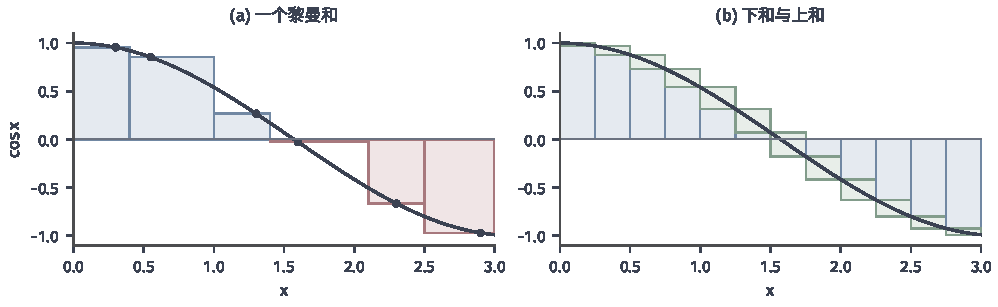
\includegraphics[width=169mm]{figures/01-mathematical-preliminaries-upper/02-real-numbers-and-univariate-functions/matplotlib/riemann-sums/figure.pdf}
 \caption{$f(x)=\cos x$在$[0,3]$上的累计。(a)不等距分割（$6$段）的一个黎曼和，黑点为各段的取样点，蓝色矩形按正号计入，红色矩形按负号计入。(b)同一函数在$12$段等距分割上的下和与上和：蓝色为下和，加上绿色部分得到上和，绿色总面积就是$U-L$。分割加细时这一差值趋于零，函数可积。图为解析示例。}
 \label{fig:ru-riemann-sums}
\end{figure*}

\subsection{可积性}
\label{sec:ru-integrability}

直接检查所有分割和取样并不方便。把每一段上可能的取样值夹在上下确界之间，就能用两个与取样无关的和控制全部黎曼和。
设$f$在$[a,b]$上有界，对分割$P$，记$m_i,M_i$为$f$在$[x_{i-1},x_i]$上的下确界与上确界，定义下和与上和
\[
 L(f,P)=\sum_im_i\,\Delta x_i,\qquad U(f,P)=\sum_iM_i\,\Delta x_i.
\]
同一分割下的任意黎曼和都满足$L(f,P)\leq S(f,P,\xi)\leq U(f,P)$。这里用确界而不用最值，因为有界函数在小段上未必取到最值。

加入新的分点时，一段被拆成几段，每个子段上的下确界不小于原段的下确界，上确界不大于原段的上确界，所以下和不减、上和不增。
任意两个分割有公共加细，因此任意下和都不超过任意上和。于是下积分$\sup_PL(f,P)$不超过上积分$\inf_PU(f,P)$。
\begin{theorem}[Darboux判据]
\label{thm:ru-darboux-criterion}
有界函数$f$在$[a,b]$上黎曼可积，当且仅当对每个$\varepsilon>0$，存在分割$P$使$U(f,P)-L(f,P)<\varepsilon$。此时积分等于上积分和下积分的共同值。
\end{theorem}
\begin{proof}
设条件成立。固定一个满足$U(f,P_0)-L(f,P_0)<\varepsilon$的分割$P_0$，设它有$k$个内分点，且$|f|\leq M$。对另一个分割$Q$，不含$P_0$分点的小段落在$P_0$的某一段内，沿用该段的上下界；
含有$P_0$分点的小段至多$k$个，总长度至多$k\|Q\|$，函数在其上的振幅至多为$2M$。所以$U(f,Q)-L(f,Q)\leq\varepsilon+2Mk\|Q\|$，$\|Q\|$足够小时小于$2\varepsilon$。
任意黎曼和与上下积分的共同值都夹在$L(f,Q)$与$U(f,Q)$之间，两者之差小于$2\varepsilon$，这正是黎曼可积的定义。
反过来，若$f$可积，取足够细的分割，在每段上分别取接近上确界与接近下确界的取样点，两组黎曼和都接近积分值，又分别接近$U$与$L$，所以$U-L$可以任意小。
\end{proof}
判据只用到实数的确界与有限分割，不需要事先知道积分值。图~\ref{fig:ru-riemann-sums}(b)中的绿色部分就是$U-L$。

由判据可以判定几类函数可积。闭区间上的连续函数一致连续，给定$\varepsilon>0$，取$\delta$使距离小于$\delta$的两点函数值相差小于$\varepsilon/(b-a)$；
网格尺度小于$\delta$时每段的振幅$M_i-m_i<\varepsilon/(b-a)$，所以$U-L<\varepsilon$。单调函数也可积：若$f$单调不减，取$n$等分，$M_i=f(x_i)$、$m_i=f(x_{i-1})$，求和相消得$U-L=(f(b)-f(a))(b-a)/n\to0$。
只有有限个间断点的有界函数同样可积：用总长度很小的有限个区间把间断点隔开，这部分对$U-L$的贡献不超过$2M$乘以总长度，其余部分按连续函数处理。

可积性有真实的限制。前面的$\mathbb I_{\mathbb Q}$在$[0,1]$的每个小区间上都同时取到$0$和$1$，所以对任意分割$L=0$、$U=1$，差值不随分割加细而减小，Darboux判据不成立。
困难不在于分割不够细，而在于函数在任意短的区间内都剧烈振荡。这类函数能否以另一种方式累计，是第~\ref{chap:measurable-functions}章的问题。

\subsection{积分的性质}
\label{sec:ru-integral-properties}

以下性质都从黎曼和直接得到。若$f,g$在$[a,b]$上可积，对同一分割和同一组取样点，$S(\alpha f+\beta g,P,\xi)=\alpha S(f,P,\xi)+\beta S(g,P,\xi)$，取极限便得线性
\[
 \int_a^b(\alpha f+\beta g)=\alpha\int_a^bf+\beta\int_a^bg.
\]
对$a<c<b$，把$c$作为分点，左右两段的黎曼和相加就是全区间的黎曼和，于是$\int_a^bf=\int_a^cf+\int_c^bf$。约定$\int_b^af=-\int_a^bf$、$\int_a^af=0$后，这个等式对$a,b,c$的任意顺序都成立。
若$f\leq g$，每个黎曼和都保持这一大小关系，所以$\int_a^bf\leq\int_a^bg$。$|f|$也可积，因为它在每段上的振幅不超过$f$的振幅；由$-|f|\leq f\leq|f|$得$\bigl|\int_a^bf\bigr|\leq\int_a^b|f|$。
乘积$fg$也可积，但积的积分一般不等于积分的积：在$[0,1]$上$\int x\cdot x\,\mathrm dx=1/3$，而$(\int x\,\mathrm dx)^2=1/4$。

保序性给出两个后面反复使用的估计。第一个是误差估计：若$|f-g|\leq\eta$在$[a,b]$上处处成立，则
\[
 \Bigl|\int_a^bf-\int_a^bg\Bigr|\leq\int_a^b|f-g|\leq\eta\,(b-a),
\]
函数的统一误差界乘以区间长度，就是积分的误差界。第~\ref{sec:ru-limit-interchange}节用它交换极限与积分，第~\ref{sec:ru-numerical-quadrature}节用它估计求积误差。
第二个是积分平均值：若$f$在$[a,b]$上连续，$m\leq f\leq M$分别为最小值与最大值，则$m\leq\frac1{b-a}\int_a^bf\leq M$，由介值定理，存在$c\in[a,b]$使
\[
 \int_a^bf(x)\,\mathrm dx=f(c)\,(b-a).
\]
$\frac1{b-a}\int_a^bf$称为$f$在$[a,b]$上的平均值，它是有限个函数值的算术平均在连续情形下的对应物。

\section{微积分基本定理}
\label{sec:ru-fundamental-theorem}

求导记录局部变化，积分记录一段范围内的累计。两者能否相互恢复，要分两个方向回答：对累计函数求导能否得到被积函数；对导数积分能否得到原函数的增量。

\subsection{累计函数的变化率}
\label{sec:ru-accumulation-derivative}

设$f$在$[a,b]$上可积，固定积分起点$a$，令
\[
 F(x)=\int_a^xf(t)\,\mathrm dt,\qquad a\leq x\leq b,
\]
称为$f$的累计函数，$t$是积分变量，$x$是$F$的自变量。若$|f|\leq M$，由区间可加性与绝对值估计，$|F(y)-F(x)|=\bigl|\int_x^yf\bigr|\leq M|y-x|$，所以累计函数总是Lipschitz连续的。
差商$(F(x+h)-F(x))/h=\frac1h\int_x^{x+h}f$恰是$f$在短区间上的平均值。若$f$在该点连续，短区间上的平均值应趋于该点的函数值。
\begin{theorem}[累计函数的导数]
\label{thm:ru-accumulation-derivative}
设$f$在$[a,b]$上可积，$F(x)=\int_a^xf$。若$f$在$c\in(a,b)$处连续，则$F'(c)=f(c)$；在端点处连续时，相应的单侧导数等于端点值。特别地，若$f$在$[a,b]$上连续，则$F'=f$处处成立。
\end{theorem}
\begin{proof}
对充分小的$h\neq0$，
\[
 \Bigl|\frac{F(c+h)-F(c)}h-f(c)\Bigr|=\Bigl|\frac1h\int_c^{c+h}\bigl(f(t)-f(c)\bigr)\,\mathrm dt\Bigr|\leq\sup_{|t-c|\leq|h|}|f(t)-f(c)|,
\]
由$f$在$c$处连续，右侧随$h\to0$趋于零。
\end{proof}
这里有三种强弱不同的结论：累计函数总是连续的；它在被积函数的连续点可微，导数等于函数值；被积函数处处连续时，它才处处可微。连续点的条件不能省略。
在$[-1,1]$上取阶跃函数$f=\mathbb I_{[0,1]}$，它只有一个间断点，因而可积，累计函数为$F(x)=\int_{-1}^xf=\max\{x,0\}$。在$x\neq0$处$F'=f$，在$x=0$处左差商恒为$0$、右差商恒为$1$，$F'(0)$不存在。
在间断点处，导数也可能存在却不等于函数值：把$f$取为只在$0$处等于$1$、其余处为$0$的函数，它的累计函数恒为零，$F'(0)=0\neq f(0)$。

\subsection{由原函数计算积分}
\label{sec:ru-newton-leibniz}

上一小节从积分出发得到导数。反过来，若已经知道一个函数的导数是$f$，能否用它计算$f$的积分？
设$f$定义在区间$I$上，若可微函数$G$在$I$上满足$G'=f$，就称$G$为$f$的\term{原函数}（antiderivative）。两个原函数的差的导数为零，由中值定理，它们在同一区间上只相差一个常数。
\begin{theorem}[Newton--Leibniz公式]
\label{thm:ru-newton-leibniz}
设$f$在$[a,b]$上连续，$G$是它在$[a,b]$上的任一原函数，则
\[
 \int_a^bf(x)\,\mathrm dx=G(b)-G(a)=:\bigl[G(x)\bigr]_a^b.
\]
\end{theorem}
\begin{proof}
由定理~\ref{thm:ru-accumulation-derivative}，累计函数$F(x)=\int_a^xf$也是$f$的原函数，所以$G=F+C$。于是$G(b)-G(a)=F(b)-F(a)=\int_a^bf$。
\end{proof}
这个公式把求定积分化为求原函数：例如$(x^3/3)'=x^2$，所以$\int_0^1x^2\,\mathrm dx=1/3$，与图~\ref{fig:ru-riemann-sums}中上下和夹逼的数值一致。

被积函数连续只是一个方便的充分条件。若$G$在$[a,b]$上连续、在$(a,b)$内可导，并且$G'$在$[a,b]$上黎曼可积（端点处任取有限值），则同样有$\int_a^bG'=G(b)-G(a)$。
证明直接用中值定理：对任意分割，在每段上选$\xi_i$使$G(x_i)-G(x_{i-1})=G'(\xi_i)\Delta x_i$，于是$G(b)-G(a)=\sum_iG'(\xi_i)\Delta x_i$恰好是一个黎曼和，令网格尺度趋零，它趋于$\int_a^bG'$。

三个概念需要分开：有原函数、黎曼可积、原函数能用基本函数写出。阶跃函数$\mathbb I_{[0,1]}$在$[-1,1]$上可积，却没有原函数：若$G'=f$，则$G$在$[-1,0]$上为常数、在$[0,1]$上为$x$加常数，在$0$处左导数为$0$、右导数为$1$，与$G'(0)=1$矛盾。
连续函数总有原函数，即它的累计函数；但原函数未必能用基本函数经有限次运算写出。$e^{-x^2}$就是这样的例子（其证明超出本书范围），它的原函数通常直接写成累计函数$\int_0^xe^{-t^2}\,\mathrm dt$。
导数不黎曼可积时能否由导数恢复函数，涉及绝对连续性，放在第~\ref{chap:measurable-functions}章讨论。

\section{积分的计算}
\label{sec:ru-integration-methods}

微积分基本定理把定积分的计算化为寻找原函数。本节先由导数表整理基本函数的原函数，再说明换元与分部积分怎样利用已知的原函数处理新的被积函数。

\subsection{基本函数的积分}
\label{sec:ru-basic-antiderivatives}

把导数表倒过来读，就得到基本函数的原函数。在所注明的区间上，
\[
 \begin{aligned}
 &\int x^\alpha\,\mathrm dx=\frac{x^{\alpha+1}}{\alpha+1}+C\ (\alpha\neq-1),&&\int\frac{\mathrm dx}x=\log|x|+C\ (x\neq0),\\
 &\int e^x\,\mathrm dx=e^x+C,&&\int a^x\,\mathrm dx=\frac{a^x}{\log a}+C\ (a>0,\ a\neq1),\\
 &\int\sin x\,\mathrm dx=-\cos x+C,&&\int\cos x\,\mathrm dx=\sin x+C,\\
 &\int\frac{\mathrm dx}{1+x^2}=\arctan x+C,&&\int\frac{\mathrm dx}{\sqrt{1-x^2}}=\arcsin x+C\ (|x|<1).
 \end{aligned}
\]
幂函数的公式在$\alpha=-1$时分母为零，这一情形单独由对数给出；$\log|x|$在$x<0$时的导数为$\frac{1}{-x}\cdot(-1)=\frac1x$，所以公式在两侧都成立。$x^\alpha$的允许区间与第~\ref{sec:ru-elementary-derivatives}节相同。

记号$\int f(x)\,\mathrm dx=G(x)+C$称为\term{不定积分}（indefinite integral），它表示$f$在一个区间上的全部原函数组成的一族函数，$C$取遍实常数；定积分$\int_a^bf$则是一个数。

若定义域由互不相连的几个区间组成，每个区间上可以取不同的常数，例如$1/x$在$(-\infty,0)$与$(0,+\infty)$上的原函数可以各取一个常数。
线性性质把复杂的被积函数拆成基本函数，例如
\[
 \int_1^2\Bigl(3x^2-\frac2x\Bigr)\,\mathrm dx=\bigl[x^3-2\log x\bigr]_1^2=7-2\log2.
\]

求出原函数后，可以求导回代核对，再检查积分区间是否落在公式成立的范围内。若忽略这一步，会得到错误的结果：$\int_{-1}^1x^{-2}\,\mathrm dx$按$[-1/x]_{-1}^1$计算得$-2$，
可是被积函数为正，积分不可能为负。问题在于$x^{-2}$在$0$处无界，不满足Newton--Leibniz公式的条件；这个积分要按第~\ref{sec:ru-improper-integrals}节的反常积分处理，实际上是发散的。

\subsection{换元法}
\label{sec:ru-substitution}

链式法则给出复合函数的导数，倒过来就是换元积分。
\begin{theorem}[换元公式]
\label{thm:ru-substitution}
设$\varphi$在$[\alpha,\beta]$上连续可微，$f$在包含$\varphi([\alpha,\beta])$的区间上连续，则
\[
 \int_{\varphi(\alpha)}^{\varphi(\beta)}f(u)\,\mathrm du=\int_\alpha^\beta f(\varphi(t))\,\varphi'(t)\,\mathrm dt.
\]
\end{theorem}
\begin{proof}
设$F$是$f$的原函数。由链式法则，$(F\circ\varphi)'=f(\varphi)\varphi'$，右侧被积函数连续，所以由Newton--Leibniz公式右边等于$F(\varphi(\beta))-F(\varphi(\alpha))$，左边也等于这个数。
\end{proof}
公式中的微分因子与积分端点一同变化：$\mathrm du$换成$\varphi'(t)\,\mathrm dt$，反映输入区间长度的伸缩；端点换成$\varphi$的对应值。定理不要求$\varphi$单调，$\varphi'<0$时端点的先后颠倒，由有向积分的约定自动处理符号。
例如$\int_0^12xe^{x^2}\,\mathrm dx$的被积函数形如$f(\varphi(x))\varphi'(x)$，取$\varphi(x)=x^2$、$f(u)=e^u$，得$\int_0^1e^u\,\mathrm du=e-1$。

另一种用法是引入新变量化简被积函数，这时要选定反函数的分支。计算四分之一单位圆的面积$\int_0^1\sqrt{1-x^2}\,\mathrm dx$，令$x=\sin\theta$。
新变量的范围取$[0,\pi/2]$，它使$\sin$从$0$递增到$1$，端点对应$0\mapsto0$、$\pi/2\mapsto1$，方向不变。在这一范围内$\cos\theta\geq0$，所以$\sqrt{1-\sin^2\theta}=\cos\theta$，开方不带负号。于是
\[
 \int_0^1\sqrt{1-x^2}\,\mathrm dx=\int_0^{\pi/2}\cos^2\theta\,\mathrm d\theta=\Bigl[\frac\theta2+\frac{\sin2\theta}4\Bigr]_0^{\pi/2}=\frac\pi4,
\]
其中用到$\cos^2\theta=(1+\cos2\theta)/2$。若把范围取成$[\pi/2,\pi]$，$\cos\theta\leq0$，开方必须写成$-\cos\theta$，同时端点方向也颠倒，结果仍是$\pi/4$；忽略其中一项就会出错。
一般可测函数在更一般的变换下的换元，放在第~\ref{chap:measurable-functions}章。

\subsection{分部积分法}
\label{sec:ru-integration-by-parts}

乘积的导数$(uv)'=u'v+uv'$含有两项。对它积分并移项，就能把其中一项的积分换成另一项。
\begin{theorem}[分部积分公式]
\label{thm:ru-integration-by-parts}
设$u,v$在$[a,b]$上连续可微，则
\[
 \int_a^bu(x)v'(x)\,\mathrm dx=\bigl[u(x)v(x)\bigr]_a^b-\int_a^bu'(x)v(x)\,\mathrm dx.
\]
\end{theorem}
\begin{proof}
由乘积法则，$uv$在$[a,b]$上连续可微且$(uv)'=u'v+uv'$，右侧两项都连续。由Newton--Leibniz公式，$\int_a^b(u'v+uv')=u(b)v(b)-u(a)v(a)$，再由积分的线性移项即得。
\end{proof}

使用时把被积函数拆成$u$与$v'$两个因子：求导后变简单的因子取作$u$，容易找到原函数的因子取作$v'$。


计算$\int_0^1xe^x\,\mathrm dx$，取$u=x$、$v'=e^x$，则$u'=1$、$v=e^x$，于是结果为$[xe^x]_0^1-\int_0^1e^x\,\mathrm dx=e-(e-1)=1$；边界项$[xe^x]_0^1=e$不能遗漏。
只有一个因子时，可以把$1$当作另一个因子：$\int_1^e\log x\,\mathrm dx$取$u=\log x$、$v'=1$，得$[x\log x]_1^e-\int_1^e1\,\mathrm dx=e-(e-1)=1$。
若反过来分配，例如对$\int x\sin x\,\mathrm dx$取$u=\sin x$、$v'=x$，剩下的积分含$x^2\cos x$，反而更复杂。

\paragraph{Taylor公式的积分余项}
分部积分的一个重要应用，是把Taylor公式的余项写成积分，从而去掉Lagrange余项中位置未知的中间点。设$f$在包含$a$与$a+h$的区间上$n+1$阶连续可微，令$\phi(t)=f(a+th)$，$t\in[0,1]$，则$\phi^{(k)}(t)=h^kf^{(k)}(a+th)$。
从$\phi(1)-\phi(0)=\int_0^1\phi'(t)\,\mathrm dt$出发，对$k\geq1$，在$\int_0^1\frac{(1-t)^{k-1}}{(k-1)!}\phi^{(k)}(t)\,\mathrm dt$中取$u=\phi^{(k)}$、$v=-(1-t)^k/k!$，分部积分给出
\[
 \int_0^1\frac{(1-t)^{k-1}}{(k-1)!}\phi^{(k)}(t)\,\mathrm dt=\frac{\phi^{(k)}(0)}{k!}+\int_0^1\frac{(1-t)^k}{k!}\phi^{(k+1)}(t)\,\mathrm dt.
\]
从$k=1$用到$k=n$，每一步分出一项$f^{(k)}(a)h^k/k!$，便得到带积分余项的Taylor公式
\begin{equation}
 f(a+h)=\sum_{k=0}^n\frac{f^{(k)}(a)}{k!}h^k+\frac{h^{n+1}}{n!}\int_0^1(1-t)^nf^{(n+1)}(a+th)\,\mathrm dt.
 \label{eq:ru-taylor-integral-remainder}
\end{equation}
若$|f^{(n+1)}|\leq M$，由$\int_0^1(1-t)^n\,\mathrm dt=1/(n+1)$，余项不超过$M|h|^{n+1}/(n+1)!$，与第~\ref{sec:ru-taylor-remainders}节的Lagrange余项给出同样的界。
积分余项不含未知点，可以直接夹逼。取$f=e^x$、$a=0$、$h=1$，余项为$\frac1{n!}\int_0^1(1-t)^ne^t\,\mathrm dt$，由$1\leq e^t\leq e$，它介于$1/(n+1)!$与$e/(n+1)!$之间；
$n=3$时$e-8/3\approx0.0516$，确实落在$1/24$与$e/24$之间。第~\ref{sec:ru-numerical-quadrature}节估计求积公式的局部误差时，同样要用Taylor展开把误差归结为高阶导数的界。

\section{反常积分}
\label{sec:ru-improper-integrals}

黎曼积分只对有限区间上的有界函数定义。下面两个积分都不在这个范围内：$\int_1^\infty x^{-2}\,\mathrm dx$的积分区间无界；$\int_0^1x^{-1/2}\,\mathrm dx$的区间有限，被积函数却在$0$附近无界。
处理办法是先在一个有限、有界的部分上积分，再让这个部分扩大，看积分是否有极限。

\subsection{无穷区间与奇点处的截断极限}
\label{sec:ru-improper-definition}

设$f$在每个$[a,b]$（$b>a$）上可积。若$\lim_{b\to+\infty}\int_a^bf$存在且有限，就称\term{反常积分}（improper integral）$\int_a^{+\infty}f$收敛，并以这个极限为它的值；否则称发散。
例如$\int_1^bx^{-2}\,\mathrm dx=1-1/b\to1$，所以$\int_1^\infty x^{-2}\,\mathrm dx=1$；而$\int_1^bx^{-1}\,\mathrm dx=\log b\to+\infty$，$\int_1^\infty x^{-1}\,\mathrm dx$发散。
被积函数在端点附近无界时，先避开这个点再取单侧极限：若$f$在每个$[a+\varepsilon,b]$上可积，定义$\int_a^bf=\lim_{\varepsilon\to0^+}\int_{a+\varepsilon}^bf$。
例如$\int_\varepsilon^1x^{-1/2}\,\mathrm dx=2-2\sqrt\varepsilon\to2$。函数在端点附近无界的点称为奇点。

区间两端都无界，或者区间内部有奇点时，要在中间取一点把积分拆开，要求每一段分别收敛，再相加；结果不依赖拆分点的选择。
这一要求防止用抵消掩盖某一侧的发散。$\int_{-\infty}^{+\infty}x\,\mathrm dx$的对称截断$\int_{-b}^bx\,\mathrm dx$恒为零，但$\int_0^{+\infty}x\,\mathrm dx$发散，所以这个反常积分发散。
同样，$\int_{-1}^1x^{-1}\,\mathrm dx$在内部有奇点，两侧$\int_0^1x^{-1}\,\mathrm dx$与$\int_{-1}^0x^{-1}\,\mathrm dx$都发散，它也发散。
对称截断的极限称为Cauchy主值，上面两个积分的主值都是$0$。主值是另一种规定，在特定问题中有用，但不能当作通常反常积分的值。

\subsection{收敛判别、绝对收敛与尾部误差}
\label{sec:ru-improper-tests}

若$f\geq0$，$\int_a^bf$随$b$单调不减，所以$\int_a^\infty f$收敛当且仅当这些截断积分有上界，与非负项级数的情形相同。由此得到比较判别：
若$0\leq f\leq g$且$\int_a^\infty g$收敛，则$\int_a^\infty f$收敛。不要求非负时，用柯西准则：$\int_a^\infty f$收敛，当且仅当对每个$\varepsilon>0$，存在$B$使$b_2>b_1>B$时$\bigl|\int_{b_1}^{b_2}f\bigr|<\varepsilon$。
比较需要基准。由原函数直接计算，
\[
 \int_1^\infty x^{-p}\,\mathrm dx\ \text{收敛}\iff p>1,\qquad\int_0^1x^{-p}\,\mathrm dx\ \text{收敛}\iff p<1.
\]
两者方向相反：无穷远处需要衰减得足够快，零点附近则不能增长得太快。

收敛的反常积分可以用有限区间上的积分近似，误差就是剩下的尾部，比较判别同时给出它的上界。例如$\int_0^\infty e^{-x^2}\,\mathrm dx$：在$x\geq b>0$上$e^{-x^2}\leq(x/b)e^{-x^2}$，所以
\[
 0\leq\int_b^\infty e^{-x^2}\,\mathrm dx\leq\frac1b\int_b^\infty xe^{-x^2}\,\mathrm dx=\frac{e^{-b^2}}{2b}.
\]
截断到$[0,3]$时，尾部误差不超过$e^{-9}/6\approx2\times10^{-5}$。剩下的有限区间积分再用第~\ref{sec:ru-numerical-quadrature}节的求积公式计算。

\paragraph{绝对收敛与条件收敛}
若$\int_a^\infty|f|$收敛，称$\int_a^\infty f$绝对收敛。由柯西准则和$\bigl|\int_{b_1}^{b_2}f\bigr|\leq\int_{b_1}^{b_2}|f|$，绝对收敛蕴含收敛。反之不成立，$\int_1^\infty\frac{\sin x}x\,\mathrm dx$是代表例子。
对截断积分分部积分，取$u=1/x$、$v'=\sin x$，
\[
 \int_1^b\frac{\sin x}x\,\mathrm dx=\Bigl[-\frac{\cos x}x\Bigr]_1^b-\int_1^b\frac{\cos x}{x^2}\,\mathrm dx.
\]
$b\to\infty$时边界项趋于$\cos1$，右边的积分由$|\cos x|/x^2\leq1/x^2$绝对收敛，所以原积分收敛。但在每个$[k\pi,(k+1)\pi]$上$\int|\sin x|/x\geq\frac2{(k+1)\pi}$，累加起来是调和级数，所以$\int_1^\infty|\sin x|/x$发散。
这个积分的收敛来自正负部分的振荡抵消，称为条件收敛，与交错级数的情形相似。反常积分收敛与一般测度意义下的可积是否相同，要等第~\ref{chap:measurable-functions}章定义了相应的积分以后才能比较。

\section{积分与极限的交换}
\label{sec:ru-limit-interchange}

用函数列逼近被积函数时，自然希望积分也随之收敛，即$\lim\int f_n=\int\lim f_n$。这是交换“积分”与“取极限”两个操作，和交换求导与极限一样，需要条件。

\subsection{函数列、级数与逐项积分}
\label{sec:ru-termwise-integration}

在固定的闭区间上，一致收敛足以保证交换。
\begin{theorem}[一致收敛与积分]
\label{thm:ru-uniform-limit-integral}
设每个$f_n$在$[a,b]$上黎曼可积，且$f_n$在$[a,b]$上一致收敛到$f$，则$f$在$[a,b]$上黎曼可积，并且$\int_a^bf_n\to\int_a^bf$。
\end{theorem}
\begin{proof}
给定$\varepsilon>0$，取$n$使$|f_n-f|<\varepsilon$处处成立。在每一小段上，$f$的上下确界与$f_n$的相差不超过$\varepsilon$，所以$U(f,P)-L(f,P)\leq U(f_n,P)-L(f_n,P)+2\varepsilon(b-a)$，
再取使$f_n$的上下和之差小于$\varepsilon$的分割，由Darboux判据$f$可积。积分的收敛来自误差估计：$\bigl|\int_a^bf_n-\int_a^bf\bigr|\leq(b-a)\sup_{[a,b]}|f_n-f|\to0$。
\end{proof}
证明的关键是“统一误差乘以区间长度”，所以区间必须有限，误差必须对所有$x$统一。逐点收敛不够，下面的窄峰说明了原因。
在$[0,1]$上令$f_n$在$[0,2/n]$上是以$(1/n,n)$为顶点的三角形，其余处为零（$n\geq2$）。每个三角形的面积都是$1$，所以$\int_0^1f_n=1$；
但对每个$x$，$f_n(0)=0$，而$x>0$时一旦$2/n<x$就有$f_n(x)=0$，所以$f_n$逐点收敛到$0$，积分的极限$1$不等于极限函数的积分$0$。
如图~\ref{fig:ru-narrow-spikes}所示，尖峰越来越窄、越来越高，总面积不变，却躲开了每一个固定的点；最大误差$\sup|f_n-0|=n$并不趋于零。

\begin{figure}[!htbp]
 \centering
 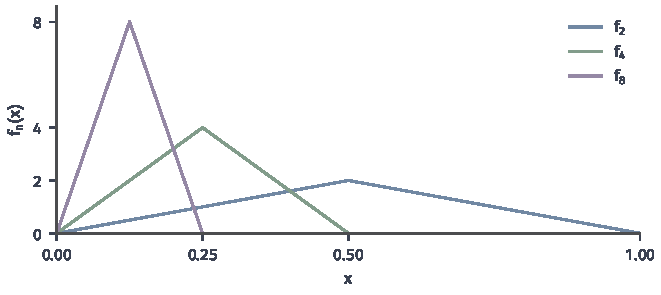
\includegraphics[width=112mm]{figures/01-mathematical-preliminaries-upper/02-real-numbers-and-univariate-functions/matplotlib/narrow-spikes/figure.pdf}
 \caption{窄峰函数列：$f_n$在$[0,2/n]$上为顶点$(1/n,n)$的三角形，其余处为零，图中画出$n=2,4,8$。每个三角形面积为$1$；固定任一$x>0$，$n>2/x$后$f_n(x)=0$，所以$f_n$逐点趋于零，积分却始终为$1$。图为解析示例。}
 \label{fig:ru-narrow-spikes}
\end{figure}

把定理用于部分和：若各项$g_k$在$[a,b]$上可积，$\sum g_k$在$[a,b]$上一致收敛，则可以逐项积分，$\int_a^b\sum g_k=\sum\int_a^bg_k$。
幂级数在收敛区间内部的闭子区间上一致收敛，所以对$|x-x_0|<R$，
\[
 \int_{x_0}^x\sum_kc_k(t-x_0)^k\,\mathrm dt=\sum_k\frac{c_k}{k+1}(x-x_0)^{k+1},
\]
逐项积分后的级数仍以$R$为收敛半径。由几何级数$\frac1{1-t}=\sum t^k$（$|t|<1$），在$[0,x]$上逐项积分得
\[
 -\log(1-x)=\sum_{k=1}^\infty\frac{x^k}k,\qquad|x|<1.
\]
这兑现了第~\ref{sec:ru-power-series-uniform}节的说法：右边的级数在$x=-1$处收敛，和函数在$[-1,1)$上连续；左边也在$x=-1$处连续，两者在$(-1,1)$上相等，在$-1$处也相等，于是$\log2=1-\frac12+\frac13-\cdots$。
同样，由$\frac1{1+t^2}=\sum(-1)^kt^{2k}$逐项积分得$\arctan x=\sum(-1)^k\frac{x^{2k+1}}{2k+1}$（$|x|<1$），右边在$x=1$处由Leibniz判别收敛，再用Abel第二定理得到$\frac\pi4=1-\frac13+\frac15-\cdots$。
这些结论都在有限闭区间上取得，不能直接推广为反常积分上的无条件交换：反常积分还多了一次截断的极限，需要另外控制。

\subsection{含参积分的连续与求导}
\label{sec:ru-parametric-integrals}

被积函数含有一个参数$y$时，积分$F(y)=\int_a^bf(x,y)\,\mathrm dx$是$y$的函数，称为含参积分。这里积分区间固定且有限，参数是唯一变化的实数。
$F$在$y_0$处是否连续，就是能否交换$y\to y_0$与积分。由上一小节的误差估计，若$y\to y_0$时$f(\cdot,y)$关于$x$一致趋于$f(\cdot,y_0)$，即$\sup_{x\in[a,b]}|f(x,y)-f(x,y_0)|\to0$，则$|F(y)-F(y_0)|\leq(b-a)\sup_x|f(x,y)-f(x,y_0)|\to0$，$F$在$y_0$处连续。
只在每个$x$处控制是不够的。把窄峰改写成连续参数：$y>0$时令$f(\cdot,y)$为$[0,2y]$上以$(y,1/y)$为顶点的三角形，$f(\cdot,0)\equiv0$。
对每个$x$，$y\to0^+$时$f(x,y)\to0$，但$y\leq1/2$时$F(y)=1$，而$F(0)=0$，$F$在$0$处不连续。

对参数求导也是一种极限交换。固定$x$，考察参数的差商$D_h(x)=[f(x,y+h)-f(x,y)]/h$，则$[F(y+h)-F(y)]/h=\int_a^bD_h(x)\,\mathrm dx$。
\begin{theorem}[积分号下求导]
\label{thm:ru-differentiation-under-integral}
设对$y$附近的每个参数，$f(\cdot,y)$在$[a,b]$上黎曼可积；并且$h\to0$时，$D_h$在$[a,b]$上一致收敛到某个函数$g$。则$F$在$y$处可导，且$F'(y)=\int_a^bg(x)\,\mathrm dx$。
\end{theorem}
\begin{proof}
任取一列$h_n\to0$，$D_{h_n}$在$[a,b]$上可积且一致收敛到$g$，由定理~\ref{thm:ru-uniform-limit-integral}，$g$可积且$\int D_{h_n}\to\int g$。由序列判据，差商$[F(y+h)-F(y)]/h\to\int g$。
\end{proof}
若$f$关于$y$可导，极限函数$g$就是偏导数$\partial f/\partial y$在$y$处的值，定理说的是$F'(y)=\int_a^b\frac{\partial f}{\partial y}(x,y)\,\mathrm dx$在差商一致收敛时成立。
以$F(y)=\int_0^1e^{xy}\,\mathrm dx$为例，参数只出现在指数因子中。由第~\ref{sec:ru-elementary-limits}节的估计$|e^u-1-u|\leq2u^2$（$|u|<1/2$），
\[
 \Bigl|D_h(x)-xe^{xy}\Bigr|=e^{xy}\Bigl|\frac{e^{xh}-1-xh}h\Bigr|\leq2e^{|y|}|h|,\qquad x\in[0,1],\ |h|<\tfrac12,
\]
所以差商关于$x$一致收敛，$F'(y)=\int_0^1xe^{xy}\,\mathrm dx$。$y\neq0$时可以直接核对：$F(y)=(e^y-1)/y$，两边都等于$(ye^y-e^y+1)/y^2$。
实际应用中更方便的充分条件是偏导数关于$(x,y)$连续，它需要多元函数的连续性，留到多元函数微积分部分（第~\ref{chap:multivariate-calculus}章）。

\section{数值求积}
\label{sec:ru-numerical-quadrature}

原函数不便求出，或者被积函数只能在有限个点上计算时，需要用有限和近似积分。黎曼和本身就是一种近似，但取样点和权重可以选得更好。
本节先确定加权积分这一对象，再分别构造矩形、梯形与Simpson公式，比较它们所需的光滑条件与误差。

\subsection{加权积分}
\label{sec:ru-weighted-integrals}

许多累计量带有权重：密度不均匀的细杆，总质量是密度乘以长度的累计；不同位置重要性不同的误差，总误差也要按位置加权。
设$w,f$在有限区间$[a,b]$上连续，称$\int_a^bw(x)f(x)\,\mathrm dx$为$f$关于权函数$w$的加权积分，$w(x)$描述位置$x$的权重。$w\equiv1$时回到普通积分。
若$w\geq0$且总权重$\int_a^bw>0$，则
\[
 \frac{\int_a^bw(x)f(x)\,\mathrm dx}{\int_a^bw(x)\,\mathrm dx}
\]
称为$f$的加权平均。由$\min f\leq f\leq\max f$乘以$w\geq0$再积分，它介于$f$的最小值与最大值之间，正如有限个数的加权平均介于最小数与最大数之间。

数值求积把积分近似为有限个函数值的加权和
\[
 \int_a^bf(x)\,\mathrm dx\approx\sum_{i=0}^nc_if(x_i),
\]
其中$x_i$称为节点，$c_i$称为求积系数。求积系数是有限个数，权函数$w$是区间上的函数，两者不要混淆；对加权积分求积时，$w$的影响会体现在系数中。
举一个连续加权平均的例子：在$[0,1]$上取$w(x)=2x$，总权重为$1$，$f(x)=x^2$的普通平均为$\int_0^1x^2\,\mathrm dx=1/3$，加权平均为$\int_0^12x\cdot x^2\,\mathrm dx=1/2$，权重偏向右端，平均值随之增大。
概率中的密度与期望正是这种计算，见\BookChapterRef{chap:random-variables}{卷2《数学准备：概率、因果与决策》的“随机变量与概率基础”章}。

下面的求积公式都把$[a,b]$等分为$n$段，步长$h=(b-a)/n$，节点$x_k=a+kh$，并用同一个算例$\int_0^1e^x\,\mathrm dx=e-1\approx1.718282$核对，取$n=4$。

\subsection{矩形求积}
\label{sec:ru-rectangle-rule}

最简单的做法是在每段上把$f$近似为常数，即用一个矩形代替这一段。取左端点、右端点或中点的函数值作为高，分别得到复合左矩形、右矩形与中点公式，例如
\[
 L_n=h\sum_{k=0}^{n-1}f(x_k),\qquad M_n=h\sum_{k=0}^{n-1}f\Bigl(x_k+\frac h2\Bigr).
\]
算例中$L_4=0.25\,(e^0+e^{0.25}+e^{0.5}+e^{0.75})\approx1.512437$，误差约$0.206$；$M_4=0.25\,(e^{0.125}+e^{0.375}+e^{0.625}+e^{0.875})\approx1.713815$，误差约$0.0045$。同样只用四个函数值，中点公式精确得多。

这些公式都是黎曼和，$f$连续时由一致连续性随$h\to0$收敛到积分。误差的阶取决于光滑条件。设$|f'|\leq M_1$，在第$k$段上$|f(x)-f(x_k)|\leq M_1(x-x_k)$，积分得局部误差不超过$M_1h^2/2$，$n$段相加得
\[
 \Bigl|L_n-\int_a^bf\Bigr|\leq\frac{M_1(b-a)}2h.
\]
中点公式多了一层抵消。设$|f''|\leq M_2$，在中点$m$处展开$f(x)=f(m)+f'(m)(x-m)+\frac12f''(\xi_x)(x-m)^2$，一次项关于中点对称，积分为零，剩下的不超过$\frac{M_2}2\int(x-m)^2=M_2h^3/24$，于是
\[
 \Bigl|M_n-\int_a^bf\Bigr|\leq\frac{M_2(b-a)}{24}h^2.
\]
端点公式的误差与$h$同阶，只需要一阶导数有界；中点公式的误差与$h^2$同阶，要求二阶导数有界。算例中两个上界分别为$e/8\approx0.34$与$e/384\approx0.0071$，都覆盖了实际误差。

\subsection{梯形求积}
\label{sec:ru-trapezoid-rule}

把每段上的$f$近似为连接两端函数值的直线，就得到梯形公式：第$k$段的积分近似为$\frac h2\bigl(f(x_k)+f(x_{k+1})\bigr)$。相加时内部节点被相邻两段共用，所以
\[
 T_n=h\Bigl[\frac12f(x_0)+f(x_1)+\cdots+f(x_{n-1})+\frac12f(x_n)\Bigr],
\]
端点系数为$h/2$，内部节点系数为$h$。算例中$T_4\approx1.727222$，误差约$0.0089$。

误差来自直线插值的偏差。设$p$是第$k$段上的直线插值，对段内固定的$x$，令$\phi(t)=f(t)-p(t)-K(t-x_k)(t-x_{k+1})$，选$K$使$\phi(x)=0$。$\phi$有$x_k,x,x_{k+1}$三个零点，两次用Rolle定理得某个$\xi$使$\phi''(\xi)=0$，即$K=f''(\xi)/2$。于是
\[
 |f(x)-p(x)|\leq\frac{M_2}2(x-x_k)(x_{k+1}-x),
\]
积分得局部误差不超过$\frac{M_2}2\cdot\frac{h^3}6=M_2h^3/12$，整体误差不超过$M_2(b-a)h^2/12$。
梯形公式与中点公式的误差都是$h^2$阶，所需条件相同，界的常数却是$1/12$对$1/24$；算例中梯形误差约为中点误差的两倍，且符号相反（梯形偏大、中点偏小），这正是凸函数的弦在图像之上、切线在图像之下。

\subsection{Simpson求积}
\label{sec:ru-simpson-rule}

用二次多项式代替直线，可以进一步提高精度。在长为$2h$的区间$[m-h,m+h]$上取端点与中点三个函数值$f_-,f_0,f_+$，过这三点的二次多项式$p(x)=A+B(x-m)+C(x-m)^2$满足$A=f_0$、$2Ch^2=f_-+f_+-2f_0$，积分得
\[
 \int_{m-h}^{m+h}p(x)\,\mathrm dx=2Ah+\frac23Ch^3=\frac h3\bigl(f_-+4f_0+f_+\bigr).
\]
中点的权重$4$来自二次项的积分。由对称性，奇次项的积分为零，所以这一公式对三次多项式也精确。把$[a,b]$分为偶数$n$段，每相邻两段组成一组，得到复合Simpson公式
\[
 S_n=\frac h3\bigl[f(x_0)+4f(x_1)+2f(x_2)+4f(x_3)+\cdots+2f(x_{n-2})+4f(x_{n-1})+f(x_n)\bigr],
\]
$n$必须是偶数，组与组之间的共用节点系数为$2h/3$。算例中$S_4\approx1.718319$，误差约$3.7\times10^{-5}$，同样只用了五个函数值。

若$f$的四阶导数连续且$|f^{(4)}|\leq M_4$，复合Simpson公式的误差满足
\[
 \Bigl|S_n-\int_a^bf\Bigr|\leq\frac{M_4(b-a)}{180}h^4,
\]
证明与梯形公式类似，用三点插值的误差估计，并利用对称性多抵消一阶\scite{math-suli2003numerical}。算例中上界为$e/(180\cdot256)\approx5.9\times10^{-5}$。
图~\ref{fig:ru-quadrature-rules}比较了三种公式：在相同的函数值数量下，Simpson公式的误差随$n$下降得最快，代价是需要更高阶的光滑性；被积函数只有低阶导数有界时，高阶公式的优势随之消失。
对反常积分，先按上一节的尾部估计截断到有限区间，再在有限区间上求积，总误差是两部分之和；被积函数在端点有奇点时，导数无界，上面的误差界都不能直接使用。

\begin{figure*}[!htbp]
 \centering
 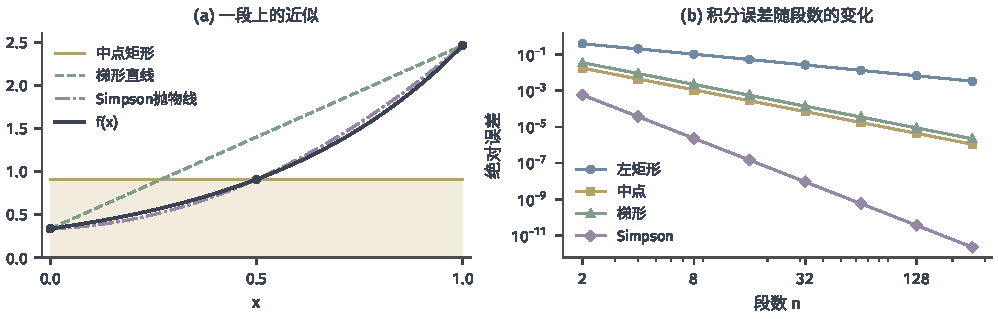
\includegraphics[width=169mm]{figures/01-mathematical-preliminaries-upper/02-real-numbers-and-univariate-functions/matplotlib/quadrature-rules/figure.pdf}
 \caption{三种求积公式的比较。(a)在一段$[0,1]$上近似$f(x)=e^{2x}/3$：中点公式用高为$f(1/2)$的矩形，梯形公式用连接两端的直线，Simpson公式用过两端与中点的抛物线，抛物线几乎与曲线重合。(b)$\int_0^1e^x\,\mathrm dx$的绝对误差随段数$n$变化，两轴均为对数刻度；左矩形、中点（与梯形）、Simpson的斜率分别约为$-1,-2,-4$，对应$h,h^2,h^4$阶误差。图为解析与双精度数值计算示例。}
 \label{fig:ru-quadrature-rules}
\end{figure*}


\FloatBarrier
\section{本章小结}
\label{sec:ru-integration-summary}

积分从有限累计出发：分割区间、在每段取样、乘以段长再求和，要求任意足够细的分割和任意取样都趋于同一个数。上下和把全部取样夹在中间，使可积性变成一个可以验证的误差条件；
连续函数、单调函数和只有有限个间断点的有界函数都可积，处处振荡的指示函数则不可积。

微积分基本定理把积分与导数联系起来：被积函数连续的点上，累计函数以它为导数；导数黎曼可积时，积分恢复端点增量。所以定积分可以由原函数计算，换元来自链式法则，分部积分来自乘积法则。

无穷区间和无界函数上的积分用截断再取极限定义，每一个问题点都要单独收敛，对称截断的抵消不能代替收敛；比较判别和幂函数基准给出尾部的误差界。

积分与极限的交换需要一致控制：在有限区间上一致收敛允许逐项积分，窄峰的例子说明逐点收敛不够；含参积分的连续与求导，也都要求参数附近的统一误差界。
数值求积用带权的有限和近似积分，矩形、梯形与Simpson公式的误差分别与步长的一次、二次和四次方成正比，前提是相应阶数的导数有界。

黎曼可积性和一致收敛的要求在两处显出了局限：逐点收敛的有界函数列，极限可能不再黎曼可积；有界函数在每个小区间上剧烈振荡时，分割无论多细都无法确定累计值。
怎样测量更一般的集合、怎样定义更一般的积分、在什么条件下可以放宽一致收敛的要求，是第~\ref{chap:measurable-functions}章与测度空间部分要回答的问题。

